%%%%%%%%%%%%%%%%%%%%%%%%%%%%%%%%%%%%%%%%%%%%%%%%%%%%%%%%%%
% Determining the document class and the input encoding: %
%%%%%%%%%%%%%%%%%%%%%%%%%%%%%%%%%%%%%%%%%%%%%%%%%%%%%%%%%%

\documentclass[paper=a4, fontsize=10.5pt, parskip=false, oneside, pointlessnumbers, leqno]{scrartcl}

\newcommand{\eqnum}{\leavevmode\hfill\refstepcounter{equation}\textup{\tagform@{\theequation}}}
% \documentclass[paper=a4, fontsize=11pt, twoside]{scrartcl}
% \documentclass[a4paper,twoside,11pt,fleqn]{article}
% \usepackage{typearea}
\typearea[2.5mm]{8}
\setlength{\textheight}{22.1cm}
% \setlength{\textwidth}{12cm}
\usepackage{lscape}

\DeclareFontFamily{OT1}{pzc}{}
\DeclareFontShape{OT1}{pzc}{m}{it}{<-> s * [1.10] pzcmi7t}{}
\DeclareMathAlphabet{\mathpzc}{OT1}{pzc}{m}{it}

\newcommand\smallO{
  \mathchoice
    {{\scriptstyle\mathcal{O}}}% \displaystyle
    {{\scriptstyle\mathcal{O}}}% \textstyle
    {{\scriptscriptstyle\mathcal{O}}}% \scriptstyle
    {\scalebox{.7}{$\scriptscriptstyle\mathcal{O}$}}%\scriptscriptstyle
  }

\usepackage{bbm}
\newtheorem{proposition}{Proposition}[section]
%\newtheorem{proof}[proposition]{Proof}
\newtheorem{proposition and definition}[proposition]{Proposition and Definition}
\newtheorem{definition}[proposition]{Definition}
\newtheorem{lemma}[proposition]{Lemma}
\newtheorem{theorem}[proposition]{Theorem}
%\newtheorem{example}[proposition]{Example}
\newtheorem{corollary}[proposition]{Corollary}
\newtheorem{remarks}[proposition]{Remarks}
\newtheorem{remark}[proposition]{Remark}
\newtheorem{assumptions}[proposition]{Assumption}
\newcommand{\timesim}{\raisebox{-2.2mm}{
\unitlength 1.00pt
\linethickness{0.5pt}
\begin{picture}(10.00,20.00)
\multiput(2.00,6.00)(0.12,0.18){50}{\line(0,1){0.18}}
\multiput(2.00,15.00)(0.12,-0.18){50}{\line(0,-1){0.18}}
\put(5.00,2.00){\makebox(0,0)[cc]{$\scriptstyle i=1$}}
\put(5.00,18.00){\makebox(0,0)[cc]{$\scriptstyle r$}}
\end{picture}
}}

\usepackage{subcaption}
% \usepackage[ansinew]{inputenc}
% \usepackage[applemac]{inputenc}
% This package enables you to input special characters---like umlauts---
% via hitting the corresponding keys on your keyboard, instead of
% having to use LaTeX commands like \"{a}, \"{o} etc.

%\usepackage{mathtools}
%\mathtoolsset{showonlyrefs=true}

%\usepackage{autonum}

%%%%%%%%%%%%%%%%%%%%%%%%%%%%%%%%%%%%%%%%%%%%%%%%%%%%%%%%
% Commands influencing the page design and typography: %
%%%%%%%%%%%%%%%%%%%%%%%%%%%%%%%%%%%%%%%%%%%%%%%%%%%%%%%%

\usepackage[USenglish, ngerman]{babel}

\usepackage{fixltx2e}

% Provides the ``\textsubscript'' command

\usepackage{ragged2e}

% Provides, among others, the \RaggedRight environment, which is \raggedright but with hyphenation enabled.

% Typeset the title, authors' names, and affiliations ragged right

\makeatletter
\def\maketitle{%
  % \null
  % \thispagestyle{empty}%
  % \vfill
  \linespread{1.05}
  \renewcommand{\thefootnote}{\fnsymbol{footnote}}
  \begin{RaggedRight}
    \leavevmode
    {\normalfont \LARGE \@title \par}%
    \vskip 20pt
    {\sffamily \bfseries \normalsize \@author \par}%
    \vskip 20pt
    {\sffamily \normalsize \@date \par}%
    \vskip 7.5pt
  \end{RaggedRight}%
  {\@thanks}
  % \vfill
  % \null
  % \cleardoublepage
  \setcounter{footnote}{0}
  }
\makeatother

\usepackage[bottom, splitrule]{footmisc}
\setlength{\footnotemargin}{0.97\parindent}
\let\oldfootnoterule\footnoterule
\renewcommand{\footnoterule}{\bigskip\oldfootnoterule\smallskip}
% Replace the asterisk in the footnotes marked with symbols by a star:
\DefineFNsymbols*{stars}{{$\star$}\dagger\ddagger\S\P\|%
                   {$\star\star$}{\dagger\dagger}{\ddagger\ddagger}}
\setfnsymbol{stars}

\let \footnoteorig \footnote
\renewcommand{\footnote}[1]{\footnoteorig{\:#1}}

% Setting up the fonts to use (needs the respective packages to be installed!):
% Just delete the percent sign "%" in front of the package combination that you want to use and
% insert a percent sign in front of the packages that you don't use:

\usepackage[flushleft, online, para]{threeparttable}
% Provides the `table notes' environment

\usepackage{amsmath, amssymb}
% This package makes additional mathematical commands and symbols available. For example, standard LaTeX
% knows a command "\begin{eqnarray} ... \end{eqnarray}" for typesetting a sequence of equations. However,
% it numbers each of the equations involved - which you might not want. Therefore, the package "amsmath"
% provides the command "\begin{eqnarray*} ... \end{eqnarray*}" which suppresses the numbering.
% \usepackage{amssymb}

\renewcommand{\dots}{\ldots{\kern -1pt}}

% \usepackage[charter, sfscaled=false]{mathdesign}
% \renewcommand{\rmdefault}{bch}
% \usepackage{charter}

\usepackage{fourier}
\DeclareMathAlphabet{\mathbfit}{T1}{fut\mathfamilyextension}{bx}{it}
\newcommand{\gammaup}{\othergamma}

%\usepackage{txfonts}
%\usepackage[LY1]{fontenc}

\newcommand{\euro}{\texteuro}

%\DeclareSymbolFont{rmcustom}{T1}\rmdefault\mddefault\updefault
%\DeclareMathSymbol{(}{\mathopen}{rmcustom}{`(}
%\DeclareMathSymbol{)}{\mathclose}{rmcustom}{`)}
%\DeclareMathSymbol{[}{\mathopen}{rmcustom}{`[}
%\DeclareMathSymbol{]}{\mathclose}{rmcustom}{`]}
%\DeclareMathDelimiter{\lbrace}{\mathopen}{rmcustom}{`\{}{largesymbols}{"08}
%\DeclareMathDelimiter{\rbrace}{\mathclose}{rmcustom}{`\}}{largesymbols}{"09}
%\DeclareMathDelimiter{\leftcurly}{\mathopen}{rmcustom}{`\{}{largesymbols}{"08}
%\DeclareMathDelimiter{\rightcurly}{\mathclose}{rmcustom}{`\}}{largesymbols}{"09}
%\renewcommand{\{}{\leftcurly}
%\renewcommand{\}}{\rightcurly}
% \DeclareMathAlphabet{\mathbfit}{T1}{chr}{bx}{it}
% \usepackage[defaultsans, scale=0.87]{opensans}
\usepackage[scaled=0.92]{helvet}
\usepackage[scaled=0.84]{beramono}
% \usepackage[defaultsans]{droidsans}
% \usepackage[defaultmono, scale=0.865]{droidmono}
% \usepackage[scaled=0.93]{PTSans}
% \usepackage{PTSansNarrow}

\usepackage{textcomp}

% sets the font of text and formulae to Utopia; sets the sans-serif and monospaced font to Bera
% \usepackage{mathptmx} \usepackage[scaled=0.9]{helvet} \usepackage{courier}
% sets the font of text and formulae to Times; sets the sans-serif font to Helvetica;
% sets the monospaced font to Courier
% \usepackage[charter]{mathdesign} \usepackage{berasans} \usepackage{beramono}
% \usepackage{charter}
% \DeclareSymbolFont{rmcustom}{T1}\rmdefault\mddefault\updefault
% \DeclareMathSymbol{(}{\mathopen}{rmcustom}{`(}
% \DeclareMathSymbol{)}{\mathclose}{rmcustom}{`)}
% \DeclareMathSymbol{[}{\mathopen}{rmcustom}{`[}
% \DeclareMathSymbol{]}{\mathclose}{rmcustom}{`]}
% \DeclareMathDelimiter{\leftcurly}{\mathopen}{rmcustom}{`\{}{largesymbols}{"08}
% \DeclareMathDelimiter{\rightcurly}{\mathclose}{rmcustom}{`\}}{largesymbols}{"09}
%\renewcommand{\{}{\leftcurly}
%\renewcommand{\}}{\rightcurly}
% sets the font of text and formulae to ITC Charter; sets the sans-serif and monospaced font to Bera
% \usepackage[osf]{mathpazo} \usepackage[scaled=0.9]{helvet} \usepackage{courier}
% sets the font of text and formulae to Palatino; sets the sans-serif font to Helvetica;
% sets the monospaced font to Courier

\frenchspacing
% By default LaTeX inserts an enlarged space after every period (.). Since the period (.) creates
% much white space anyway, enlarging the subsequent space is unnecessary. The \frenchspacing command
% suppresses the insertion of additional white space.

\flushbottom  % forces the bottom text lines on each page to be horizontally aligned

\sloppy  % less punishment for large whitespace within text lines

% \usepackage[activate]{pdfcprot}
% \usepackage[protrusion=true, factor=1200, expansion=compatibility]{microtype}
\usepackage[protrusion=true, expansion=false, kerning=true]{microtype}
% This package enables so-called hanging punctuation. That is, when a punctuation sign like ":", ".", "-" etc.
% is found at the beginning or end of a line, it is protruded a little into the page margin. This leads to
% so-called "optical margin alignment", because the protrusion makes the margin alignment look straighter.
\SetExtraKerning[unit=space]
  {encoding={*}, family={*}, series={*}, size={*, footnote size}}
  {\textemdash={325,325}}

\usepackage{enumitem}
\setlist[enumerate]{leftmargin=\parindent, listparindent=\parindent, parsep=0pt, labelsep=0.42\parindent}

% \def\semismall{\@setfontsize{\semismall}{10.25pt}{13.5pt}}
\renewenvironment{quote}
                 {\list{}{\leftmargin\parindent \rightmargin\parindent}%
                  %\small
                  \setlength{\baselineskip}{2.8ex}\item\relax}
                 {\endlist}

\newenvironment{tightitemize}{
  \begin{list}{\makebox(5.5,4.5)[t]{$\scriptstyle \bullet$}}{%
    \advance\partopsep  by \topsep
    \setlength{\topsep}{0.75ex}
    \setlength{\itemsep}{0in}
    \setlength{\parsep}{0em}
    \setlength{\leftmargin}{\parindent}
    \setlength{\rightmargin}{0in}
    \setlength{\itemindent}{0in}
  }
}
{\end{list}}

\newcommand{\highlight}[1]{\textcolor{medred}{[[\:\textbf{#1}\:]]}}

% Packages to influence table layout:
\usepackage{tabularx}
% \usepackage{tabulary}
\usepackage{booktabs}
\heavyrulewidth=.05em
% \belowbottomsep=-2.5pt
\usepackage{multirow}
% Enables the "\multirow" command for typesetting cells inside tables which span several rows.
% \usepackage{colortbl}

% A package to change the formatting of the table of contents:
\usepackage[titles]{tocloft}
\setlength{\cftbeforesecskip}{1ex}
\renewcommand{\cftsecfont}{\sffamily\bfseries\selectfont}
\renewcommand{\cftsecpagefont}{\sffamily\bfseries\selectfont}
\cftsetrmarg{27.5pt}
\cftsetpnumwidth{22.5pt}
\makeatletter
  \renewcommand{\@tocrmarg}{27.5pt plus1fil}
\makeatother

% A package to change the formatting of the captions for tables and figures:
%\usepackage{caption}
%\DeclareCaptionLabelSeparator{colon}{:\ \ \ }
%\captionsetup{format=hang, labelsep=colon, justification=RaggedRight, font={sf, small}, labelfont=bf}
% Formatting the captions:
\usepackage{caption}
\captionsetup{
  figureposition=below,
  tableposition=above,
  format = plain,
  labelsep=period,
  margin = \parindent,
  font = {sf, footnotesize},
  labelfont = {bf},
  justification = centering
}
% \usepackage[margin=\parindent, justification=centering, font=small]{caption}[2007/04/16]

%% Disable single lines at the start of a paragraph (Schusterjungen)
%\clubpenalty = 10000
%% Disable single lines at the end of a paragraph (Hurenkinder)
%\widowpenalty = 10000 \displaywidowpenalty = 10000
\usepackage[all]{nowidow}

\renewcommand{\bottomfraction}{0.99}
\renewcommand{\topfraction}{0.99}

\linespread{1}

% \include{letterspacing}
% \newcommand{\caps}[1]{\scalebox{0.97}{\letterspace to 1.06\naturalwidth{#1}}}
\newcommand{\caps}[1]{\scalebox{0.97}{\textls[50]{#1}}}
\newcommand{\code}[1]{\texttt{#1}}
% \newcommand{\code}[1]{\scalebox{0.98}{\textls[5]{\texttt{#1}}}}
% The \textls command is only available if microtype has been loaded

\newcommand{\dbreak}{\hspace{0pt}}	% discretionary line break


%%%%%%%%%%%%%%%%%%%%%%%%%%%%%%%%%%%%%%%%
% Commands influencing the PDF output: %
%%%%%%%%%%%%%%%%%%%%%%%%%%%%%%%%%%%%%%%%

\usepackage[pdftex]{graphicx}
\usepackage[table]{xcolor}
\definecolor{UBonnBlue}{RGB}{000,066,145}
\definecolor{DarkWarmGrey}{RGB}{105,105,090}
\definecolor{WarmGrey}{RGB}{139,138,125}
\definecolor{darkblue}{rgb}{0.00,0.00,0.50}
\definecolor{medred}{rgb}{0.75,0.00,0.00}
\definecolor{darkred}{rgb}{0.70,0.00,0.00}
\definecolor{customgreen}{rgb}{0.2,0.6,0.00}
\usepackage[pdftex, pdftitle={Cognitive Load Increases Risk Aversion},
pdfauthor={Holger Gerhardt, Guido Biele, Harald Uhlig, Hauke~R. Heekeren}, pdfsubject={}, bookmarks=true, bookmarksopen=true,
bookmarksnumbered=true, bookmarksopenlevel=2, colorlinks=true, pdfpagemode=UseOutlines, pdfview=Fit,
pdfstartview=Fit, pdffitwindow=false, linkcolor=UBonnBlue, citecolor=UBonnBlue,%
% backref=page,
urlcolor=UBonnBlue]{hyperref}
\urlstyle{same}   % Sets URLs in the text font instead of the typewriter font
% \renewcommand{\url}[1]{\href{#1}{#1}}
% \usepackage{memhfixc}
% Only needed when using the "memoir" class

% Enclose the back references in the bibliography to the pages on which a reference is cited
% in square brackets (Econometrica style)
% \let \backrefold \backref
% \renewcommand*{\backref}[1]{[\backrefold{#1}]}

% Influencing the color and font sizes of the headings:
\addtokomafont{sectioning}{\color{UBonnBlue}}
% \addtokomafont{sectioning}{\color{darkred}}
% \addtokomafont{sectioning}{\rmfamily}
% \addtokomafont{section}{\fontseries{l}\selectfont\large} % for OpenSans only
% \addtokomafont{subsection}{\fontseries{sb}\selectfont\normalsize} % for OpenSans only
\addtokomafont{section}{\large}
\addtokomafont{subsection}{\normalsize} % for OpenSans only
% \addtokomafont{subsubsection}{\normalsize \mdseries}
% \addtokomafont{subsubsection}{\normalsize \rmfamily}

% For AEA.cls:
%\renewcommand{\subsubsection}[1]{%
%\addtocounter{subsubsection}{1}%
%\bigskip\textit{\arabic{subsubsection}.~#1}---}

% For scrartcl.cls:
\renewcommand{\subsubsection}[1]{%
\addtocounter{subsubsection}{1}%
\bigskip\noindent\emph{\hspace{\parindent}\arabic{subsubsection}.~#1}---\hspace{0pt}}
\newcommand{\runinhead}[1]{%
\bigskip\noindent\emph{\hspace{\parindent}#1.}---\hspace{0pt}}

% Hanging/constant-width section numbers:
\makeatletter
\def\@seccntformat#1{%
       \protect%
       \hspace{-31pt}%
       \makebox[31pt][l]{%
              \csname  the#1\endcsname%
              %\quad
              }%
   }
\makeatother


%%%%%%%%%%%%%%%%
% Commenting commands %
%%%%%%%%%%%%%%%%


\setlength{\marginparwidth}{4.1cm}
\setlength{\marginparsep}{0.4cm}
\setlength{\marginparpush}{0.4cm}
%\newcommand{\comment}[2]{\setbox99=\hbox{\textbf{\v{|}}}\textcolor{darkred}{\hspace{-0.75pt}\textbf{\raisebox{1.5pt}{\v{}}\hspace{-\wd99}\raisebox{0.5pt}{|}}}\hspace{0.75pt}\hspace{-\wd99}\marginpar{\RaggedRight \sffamily \footnotesize \setlength{\baselineskip}{2.35ex} \textcolor{darkred}{\textbf{#1}\\ #2}}}

\newcommand{\comment}[2]{\setbox99=\hbox{\textbf{\v{ }}}\makebox[0pt][l]{\hspace{-1.35pt}\textcolor{darkred}{\textbf{\raisebox{1.75pt}{\v{ }}\hspace{-0.827\wd99}|}}}\marginpar{\RaggedRight \sffamily%
%\fontseries{l}\selectfont
\footnotesize \setlength{\baselineskip}{2.35ex} \textcolor{darkred}{\textbf{%
%\fontseries{sb}\selectfont
#1}\\ #2}}}
% \renewcommand{\comment}[2]{}{}

\newcommand{\commentgreen}[2]{\setbox99=\hbox{\textbf{\v{ }}}\makebox[0pt][l]{\hspace{-1.35pt}\textcolor{customgreen}{\textbf{\raisebox{1.75pt}{\v{ }}\hspace{-0.827\wd99}|}}}\marginpar{\RaggedRight \sffamily%
%\fontseries{l}\selectfont
\footnotesize \setlength{\baselineskip}{2.35ex} \textcolor{customgreen}{\textbf{%
%\fontseries{sb}\selectfont
#1}\\ #2}}}
% \renewcommand{\commentgreen}[2]{}{}

%%%%%%%%%%%%%%%%%%%%%%%%%%%%%%%%%%%%
% Some user-defined math commands: %
%%%%%%%%%%%%%%%%%%%%%%%%%%%%%%%%%%%%

% The following line introduces a new command which makes it easy to typeset vectors and matrices,
% surrounded by regular (round) parentheses:
\newcommand{\rdmatrix}[1]{\left(\,\begin{matrix}#1\end{matrix}\,\right)}
% The same for vectors/matrices surrounded by square brackets:
\newcommand{\sqmatrix}[1]{\left[\,\begin{matrix}#1\end{matrix}\,\right]}
% Putting a backslash in front of "exp", "lim", "max" etc. makes LaTeX recognize the respective mathematical
% expression as a function or operator. These are then not set in italics but upright. It improves
% intellegibility of mathematical expressions to set the following operators upright, too:
%\newcommand{\E}{\mathrm{E}}
%\EE
\DeclareMathOperator{\bias}{Bias}
\DeclareMathOperator{\var}{Var}
\DeclareMathOperator{\tr}{tr}
%\DeclareMathOperator{\sup}{sup}
\DeclareMathOperator{\cov}{Cov}


\newcommand{\equals}{\;=\;}
\newcommand{\mdash}{{\tiny{ }}---{\tiny{ }}}

\usepackage{commath}
%\usepackage{amsmath,amsfonts}
\DeclareMathOperator{\spn}{span}



\usepackage{rotating}

\usepackage{abstract}
\renewcommand{\absnamepos}{flushleft}
\renewcommand{\abstractnamefont}{\sffamily \bfseries \normalsize}

\usepackage{multicol}


%%%%%%%%%%%%%%%%%%%%%%%%%%%%%%%%%%%%%%%%%%%
% Commands connected to the bibliography: %
%%%%%%%%%%%%%%%%%%%%%%%%%%%%%%%%%%%%%%%%%%%

% The following package has to be loaded to be able to use the "Econometrica" bibliography style.
\usepackage{natbib}
% \usepackage[longnamesfirst]{natbib}
% \renewcommand{\harvardand}{and}
% \newcommand{\harvardand}{and}
% Since the "\cite" command puts parentheses around the cited work - which one doesn't want in most cases -
% it is useful to redefine the meaning of "\cite"
% \newcommand{\citep}[1]{(\citeauthor{#1}, \citeyear*{#1})}
% \newcommand{\cite}[1]{\citeauthor{#1}, \citeyear*{#1}}
% \renewcommand{\cite}[1]{\citeasnoun{#1}}


%%%%%%%%%%%%%%%%%%%%%%%%%%%%%%%
% Now the actual text begins: %
%%%%%%%%%%%%%%%%%%%%%%%%%%%%%%%

\usepackage{hyperref}
\hypersetup{pdfstartview={XYZ null null 0.88}}
\newcommand{\EE}{\mathop{\mbox{\sf E}}}

\begin{document}

\selectlanguage{USenglish} \frenchspacing
% \pagenumbering{roman}
% Numbers the pages of the front matter by "i", "ii", "iii", "iv" and so on.

\begin{titlepage}

% \def\blfootnote{\xdef\@thefnmark{}\@footnotetext}

\title{Functional Principal Component Analysis \\for Derivatives of High-Dimensional \\Spatial Curves \thanks{$\:$The financial support from the German Research Foundation for the joint project no. 70102424 "Functional Principal Components for Derivatives and Higher Dimensions", between Humboldt-Universit\"at zu Berlin and Rheinische Friedrich-Wilhelms-Universit\"at Bonn, is gratefully acknowledged. We would like to thank as well the Collaborative Research Center 649 ``Economic Risk'' for providing the data and the International Research Training Group (IRTG) 1792 ``High-Dimensional Non-Stationary Time Series Analysis'', Humboldt-Universit�t zu Berlin for additional funding.}}

\author{Maria Grith,\textsuperscript{\!1}
Wolfgang K. H{\"a}rdle,\textsuperscript{\!1,3} 
Alois Kneip \textsuperscript{\!2} and
Heiko Wagner\textsuperscript{\,2} \\[7.5pt]
\normalfont \scriptsize \sffamily
\textsuperscript{\phantom{0}1}\,Ladislaus von Bortkiewicz Chair of Statistics and C.A.S.E. - Center for Applied Statistics and Economics, School of Business and Economics, Humboldt-Universit\"at zu Berlin, Spandauer Stra{\ss}e 1, 10178 Berlin, Germany \\
\scriptsize \sffamily
\textsuperscript{\phantom{0}2}\,Institute for Financial Economics and Statistics, Department of Economics, Rheinische Friedrich-Wilhelms-Universit\"at Bonn, Adenauerallee 24-26, 53113 Bonn \\
\scriptsize \sffamily
\textsuperscript{\phantom{0}3}\,Sim Kee Boon Institute for Financial Economics, Singapore Management University, 81 Victoria Street, Singapore 188065
}
\date{\medskip This version: \today}
\maketitle

\medskip

\setlength{\absleftindent}{0pt}
\setlength{\absrightindent}{0pt}
\setlength{\abstitleskip}{-\absparindent}
\setlength{\columnsep}{0.95pc}

\let\hyphenpenaltyorig=\hyphenpenalty
\let\toleranceorig=\tolerance
\begin{abstract}   \hyphenpenalty=10 \tolerance=500
\noindent %Our paper addresses the challenge of recovering the derivatives of high-dimensional spatial noisy curves. We adapt the functional principal component analysis (FPCA) to this task using dual method and illustrate two approaches to obtain the derivatives. We compare their asymptotic performance and finite sample behavior, focusing on the computational efficiency. In a financial application that uses observed call option prices we estimate the state price density (SPD) surfaces and find that two components dominate their variability. %and extract the economic content embedded in their dynamics.  
%one-dimensional Functions=infinite dimensional vectors; multidimensional; joint functional structure. 
%In this paper we address the challenge of estimating smooth derivatives of high-dimensional spatial curves  with joint functional variation from noisy discrete observations using a parsimonious representation of their variation. We present two related approaches based on the functional principal component analysis (FPCA) and compare their asymptotic performance and finite sample behavior, focusing on the computational efficiency. In a simulation and empirical study, we illustrate the methodology to estimate state price density (SPD) surfaces from call option prices.
%We estimate smooth derivatives of high-dimensional spatial curves  that display joint functional variation using two related approaches based on the functional principal component analysis (FPCA), and compare their asymptotic performance and finite sample behavior, focusing on the computational efficiency. In a simulation and empirical study, we illustrate the methods by the estimation of state price density (SPD) surfaces from call option prices.
We present two approaches based on the functional principal component analysis (FPCA) to estimate smooth derivatives of noisy and discretely observed high-dimensional spatial curves.  %that display joint functional variation. 
One method is based on the eigenvalue decomposition of the covariance operator of the derivatives and the other assumes the operator of the curves. To handle observed data, both approaches rely on local polynomial regressions. We analyze the requirements under which the methods are asymptotically equivalent, and establish that the first approach requires very strong smoothness assumptions to achieve similar convergence rates to the second one. %The implementation of the second approach has also computational advantages. 
If the curves are contained in a finite-dimensional function space, we show that using both our methods provides better rates of convergence then estimating the curves individually. We illustrate the methodology in a simulation and empirical study, in which we estimate state price density (SPD) surfaces from call option prices. %This study extends that of previous researchers who have analyzed implied volatility surfaces in the cross- section of options. 
We identify three main components, which can be interpreted as volatility, skewness and convexity factors. We also find effects introduced by the term structure variation. 


%Our paper addresses the challenge of recovering the derivatives of high-dimension spatial noisy curves. We adapt the functional principal component analysis (FPCA) to the case of derivatives using the dual method and show how to estimate high-dimensional FPCA computationally efficient. We present two alternative methods to obtain the derivatives and compare their performance asymptotically and in finite sample. In a financial application that uses observed call option prices we estimate the state price density (SPD) surfaces and find that two components are sufficient to explain most of their variability. %and extract the economic content embedded in their dynamics.  

%This allows us to reduce the model complexity and express curves variability in terms of few principal components and loadings that can be used for further analysis.

\medskip

\hyphenpenalty=\hyphenpenaltyorig \tolerance=\toleranceorig





\noindent \emph{Keywords:\:} functional principal component, dual method, derivatives, high-dimensional spatial curves, state price densities

\medskip

\noindent \emph{JEL codes:\:} C13, C14, G13

\end{abstract}

\thispagestyle{empty}
% Suppresses the needless output of the page number on the title page.

\end{titlepage}

\pagenumbering{arabic}
% Sets the page numbering to the usual numbers: "1", "2", "3", "4" and so on.

\setcounter{page}{2}

\setlength{\baselineskip}{2.9ex}
\setlength{\parindent}{2.9ex}
% This influences the line spacing in the footnotes
\linespread{1.075}

% \setlength{\mathindent}{\parindent}	% only if ``fleqn'' option is used

% Increases line spacing a bit, which improves legibility. This is especially useful for texts containing
% mathematical formulae, in order to prevent subscripts and superscripts in the formulae to collide with
% the following and previous lines, respectively.


\section{Introduction}

Over the last two decades, functional data analysis became a popular tool to handle data entities that are functions. Usually, discrete and noisy versions of them are observed. Oftentimes, these entities are high-dimensional spatial objects. Examples include brain activity recordings generated during fMRI or EEG experiments, e.g., \cite{majer:15}. %, environmental or climatological maps.  
In a variety of applications though the object of interest is not directly observable but it is a function of the observed data.  Typical examples in the financial applications include functionals that can be retrieved from the observed prices by means of derivatives, such as implied state price density, e.g., \cite{Schienle:12}, pricing kernel, e.g., \cite{Gr:13} or the market price of risk, e.g.,  \cite{Lopez:12}. Motivated by such data analysis situations, we address the problem of estimating high-dimensional spatial curves that are not empirically observable but can be recovered from the existing discrete and noisy data by means of derivatives. %An example of such an instance that motivates our present study are the SPDs implied by option prices. SPDs are continuous versions of Arrow Debreu prices that pay one unit of currency if one state is realized and zero otherwise. %Considered basic securities, they are not traded over exchanges but can be calculated from the prices of existing securities. 

%The usefulness of knowing the shape and dynamics of SPDs derives, among others, from the possibility of fair pricing of exotic contingent claims because they are assumed to reflect equilibrium conditions on the market, see pricing under the risk neutral rule, e.g. \cite{Harrison:79}. Furthermore, due to the forward-looking perspective, they are used to estimate the physical density of the underlying asset by incorporating the adjustments for risks by means of pricing kernel, e.g. \cite{Anagnou:02}, \cite{Bliss:04}, \cite{Alonso:09}, \cite{Duca:14}. In addition, the exchanges calculate volatility indexes, such as VIX for S$\&$P 500 or VDAX for DAX 30, that reflect the market expected forward volatility. Also known by the investors as 'fear indices' they are computed from option prices, with a link to but not a straight forward interpretation of the implied densities. 

%These adjustments require the understanding of behavioral risk patterns on the market - through the aggregate measures of preferences and beliefs - and this is possible by linking the implied state price to the physical densities, see \cite{hens:12}, \cite{Bakshi:10}, \cite{Polkovnichenko:12}, \cite{Kra:14}.
Functions, which are objects of an infinite-dimensional vector space, require specific methods that allow a good approximation of their variability with a small number of components. FPCA is a convenient tool to address this task because it allows to explain complicated data structures with only a few orthogonal principal components that fulfill the optimal basis property in terms of its $L^2$ accuracy. These components are given by the Karhunen-Lo{\`e}ve theorem, see for instance \cite{Bosq:2000}. %In the one-dimensional case it is also easy to implement. 
In addition, the corresponding principal loadings to this basis system can be used to study the variability of the observed phenomena. %, for example in a time series framework. In addition, depending on the application the corresponding principal scores can be interpreted, for example in a time series framework.
%The mathematical basis for the Karhunen-Lo{\`e}ve decomposition is given by the Hilbert-Schmidt theorem. % from the functional analysis theory. In the last years a lot of effort has been done to lay a theoretical foundation for the use of these insights in a statistical context. 
An important contribution in the treatment of the finite dimensional PCA was done by \cite{Pousse:82}, followed by subsequent studies that fostered the applicability of the method to samples of observed noisy curves. \cite{Besse:86}, among others, derived theoretical results for observations that are affected by additive errors. Some of the most important contributions for the extension of the PCA to functional data belong to \cite{cardot1999functional}, \cite{Cardot2007}, \cite{Vieu2006}, \cite{Mas2002117} and \cite{mas2008local}.
To date, simple, one-dimensional spatial curves are well understood from both numerical and theoretical perspective. In the one-dimensional case FPCA is also easy to implement. High-dimensional objects, with more complicated spatial and temporal correlation structures, or not-directly observable functions of these objects, such as derivatives, lack a sound theoretical framework. Furthermore, the computational issues are not negligible in high-dimensions. 

To our best knowledge, FPCA for derivatives has been tackled by \cite{Hall:09} and \cite{Mueller:2009}. The first study handles one-dimensional directional derivatives and gradients. The second paper analyses a particular setup in one-dimension where the observations are sparse. This method can be applied to non-sparse data but may be computationally inefficient when dealing with large amount of observations per curve. There are no studies of derivatives using FPCA in more than one spatial dimension. For the study of observed functions, there are a series of applied papers for the two-dimensional case, see \cite{Cont:02} for an application close to our empirical study. Other complicated attempts to implement FPCA when the object of interest are the observed functions, rather than their derivatives, have been done in more than two dimensions, in particular in the area of brain imaging. For example, \cite{Zipunnikov:11} split the recorded data into smaller parts to make it manageable. The method called multilevel FPCA has been developed through previous studies, see \cite{Staicu01042010}, \cite{di2009multilevel}, and is well suited to analyze different groups of individuals. However, a thorough derivation of the statistical properties of the estimators is missing in these papers.

%To our knowledge, the functional data analysis for derivatives has been done by \cite{Mueller:2009}, in a particular type of application in one-dimension where the observations are sparse. When applied to non-sparse data, the methodology is inefficient. Another paper by \cite{Hall:09} handles one-dimensional directional derivatives and gradients. There are no studies of derivatives using FPCA in more than one-dimension. 

%Particularly when high-dimensional data is present, the computational aspect is not negligible. For every additional dimension exponentially many observations are needed to get the same rate of convergence. There is no straightforward way to generalize the commonly used procedures to compute the FPCA to the higher dimensional case, without getting into computational trouble. Complicated attempts has been done for example by \cite{Zipunnikov:11} where the data is split into smaller parts to be still calculable. 

%A way to handle large amounts of observations was proposed by \cite{Benko:2009} where the duality relation is used for one-dimensional curves. Computational efficiency is essential with increasing spatial dimensions and the dual method performs better when the number of curves is smaller than the number of the discrete observations per curve. We will also use this approach here.

In this paper, we aim to fill in the existent gaps in the literature on FPCA for the study of derivatives of functions in high-dimensional spaces. We present two alternative methods to obtain the derivatives. %and to apply the newly developed framework to the study of SPDs.
%The rest of the paper is organized as following: The theoretical framework, estimation procedure and statistical properties will be derived through sections \ref{t2} and \ref{t3} for general functions. Our empirical study in section \ref{t4} is guided by the estimation and dynamics analysis of option implied SPDs in a simulation study and real data example. Section \ref{t5} concludes. 
The paper is organized as following: the theoretical framework, estimation procedure and statistical properties are derived through Section \ref{t2}. Our empirical study in Section \ref{t4} is guided by the estimation and the dynamics analysis of the option implied state price densities. It includes a simulation study and a real data example. %Section \ref{t5} concludes. 


%\color{red}VIX = constructed by CBOE based on some continuous-time theory ??? Zhaogang 2013\color{black}

\section{Methodology}\label{t2}

%Handling infinite-dimensional data structures requires specific methods that allow the representation of their variability with a small number of components. Karhunen-Lo{\`e}ve decomposition is a convenient tool to address this task; it allows to explain complicated data structures with only a few principal components. In addition, the corresponding principal scores can be used to study the evolution of the observed phenomena, for example in a time series framework. %In addition, depending on the application the corresponding principal scores can be interpreted, for example in a time series framework.

%The mathematical basis for the Karhunen-Lo{\`e}ve decomposition is given by the Hilbert-Schmidt theorem. % from the functional analysis theory. In the last years a lot of effort has been done to lay a theoretical foundation for the use of these insights in a statistical context. 
%An important contribution in this context has been done by \cite{Pousse:82}, followed by consequent studies that fostered the applicability of the method to samples of observed noisy curves. \cite{Benko:2009} and \cite{Besse:86}, among others, derived theoretical results for observations that are effected by additive errors. 

%To date, simple, one-dimensional structures are well understood from both numerical and theoretical perspective. High-dimensional structures, with more complicated spatial and temporal correlation structures, or derivatives lack a sound theoretical framework. In addition, the computational issues are not negligible. A few papers have tackled the indirectly observed curves estimation. \cite{Hall:09} handle one-dimensional directional derivatives and gradients. \cite{Mueller:2009} analyze a particular setup in one-dimension where the observations are sparse. When applied to non-sparse data, this methodology is computationally inefficient. Though there are no studies of derivatives using FPCA in more than one-dimension. For the study on nonderivatives, there are a series of applied papers for the two-dimensional case, see \cite{Cont:02} for an application close to our empirical study. Complicated attempts to implement FPCA for nonderivatives in more that two dimensions has been done, for example by \cite{Zipunnikov:11}, where the data is split into smaller parts to make it manageable. However, a thorough derivation of the statistical properties of these estimators is missing.

%To our knowledge, the functional data analysis for derivatives has been done by \cite{Mueller:2009}, in a particular type of application in one-dimension where the observations are sparse. When applied to non-sparse data, the methodology is inefficient. Another paper by \cite{Hall:09} handles one-dimensional directional derivatives and gradients. There are no studies of derivatives using FPCA in more than one-dimension. 

%Particularly when high-dimensional data is present, the computational aspect is not negligible. For every additional dimension exponentially many observations are needed to get the same rate of convergence. There is no straightforward way to generalize the commonly used procedures to compute the FPCA to the higher dimensional case, without getting into computational trouble. Complicated attempts has been done for example by \cite{Zipunnikov:11} where the data is split into smaller parts to be still calculable. 

%A way to handle large amounts of observations with joint functional structure was proposed by \cite{Benko:2009} where the duality relation is used for one-dimensional curves. Computation efficiency is essential with increasing dimensions and the dual method performs better when the number of curves is smaller than the number of the discrete observations per curve. In this paper, we generalize this procedure to the case of derivatives in high-dimensions. Next, we will present two alternative methods to obtain the derivatives and in the subsequent two sections we will explain their comparative performance in terms of asymptotics and finite sample in a simulation study.


%In our empirical study we are guided by a finance application in which we want to explain the variability of option implied SPDs 

% in which we want to explain the variability of option implied SPDs through dynamic parameters (principal scores) that can be interpreted within a time series framework. 

%ADD STH ABOUT APPLICATION HERE!


%In this paper we aim to recover the derivatives of high-dimensional noisy curves, as well as to summarize them by few principal components and to explain their variability through dynamic parameters that can be interpreted within a time series framework. To achieve this goal we employ a functional data analysis (FDA) method based on the Karhunen-Lo{\`e}ve decomposition of a random curve via a set of orthonormal basis functions gained from the covariance operator. In particular, we will adapt the functional principal component analysis (FPCA) for curves to the case of their derivatives.

%The main assumption for performing this decomposition is that the curves are square integrable and their derivatives exist. One situation when this condition is fulfilled if the case of continuous phenomenon that can be represented as smooth functions. For a finite number of curves observed without errors the Karhunen-Lo{\`e}ve decomposition is applied to the sample counterpart of the covariance operator, as shown in \cite{Hall:2006}. If these curves are additionally observed at discrete points with noise, as it is often the case in practice, smoothing is required at some stage, see \cite{Benko:2009} or (reference Silverman for ex.) for additional details. 

%Our approach is a generalization of the approach presented by \cite{Benko:2009}. They introduce a new method for the estimation of principal components of functions from discrete noisy data, based on the duality relation for matrices (see härlde book ref). One advantage of using this method is that no smoothing of individual curves is required to obtain an asymptotically unbiased estimator for the dual matrix of the covariance operator. Consequently, this estimation method doesn't suffer of the potential biases and inconsistencies introduced by smoothing involved in the application of other famous method e.g.(reference) to the noisy data. In addition, the method is computationally more efficient when the sample size is smaller than observation points (why, reference). 

%To apply standard approaches which are based of decomposing the covariance directly, to higher dimensions has several problems: computational effort for computing the covariance matrix and the eigenvalues decomposition increases exponentially with every additional dimension. (why, reference) Besides, it is not clear how one can adapt the standard method to the high-dimensional case, in particular with respect to the derivation of theoretical properties of the estimators. 

%To our knowledge, the functional data analysis for derivatives has only been done by \cite{Mueller:2009}, and only in a particular type of application with sparse data in one-dimension. (explain method) When applied to non-sparse data, the methodology is inefficient and causes not very good convergence rates (reference). There are no studies of derivatives using FPCA in more dimensions. 

%(the advantage of analyzing all the curves together. estimating them using FPCA. signal to noise ratio, leveling down the noise by averaging, assumptions about the curves as being realizations from a stationary process)

%The paper is organized as follows: 
%\subsection{Karhunen-Lo{\`e}ve decomposition and derivatives of (multivariate) functions}
\subsection{Two approaches to the derivatives of high-dimensional functions using FPCA}
%\subsection{Theoretical underpinnings}
The representation of derivatives of high-dimensional spatial curves requires a careful choice of notation. In this section, we review the FPCA from a technical point of view and make the reader familiar with our notations. 

Let $X$ be a centered smooth random function in $L^2([0,1]^g)$, where $g$ denotes the spatial dimension, with finite second moment $\int_{[0,1]^g} \EE\left[X(t)^2 \right]dt < \infty$ for $t=(t_1, \ldots, t_g)^{\top}$. %Here, we consider centered functions. %if non-centered curves are assume than there is a need to additionally subtract $E(Y)$. 
The underlying dependence structure can  be characterized by the covariance function $\sigma(t,v)\stackrel{\operatorname{def}}{=}\EE\left[X(t)X(v)\right]$ and
 the corresponding covariance operator $\Gamma$% applied to some function $\vartheta \in L^2([0,1]^g)$
 \begin{equation*}
%\Gamma \vartheta(t)=\int_{[0,1]^g}\sigma(t,v)\vartheta(v)dv,
(\Gamma \vartheta)(t)=\int_{[0,1]^g}\sigma(t,v)\vartheta(v)dv.
\end{equation*}
%Under weak conditions $\Gamma$ is a Hilbert-Schmidt operator and possesses a countable number of non-negative eigenvalues. 
Mercer's lemma guarantees the existence of a set of eigenvalues $\lambda_1\geq \lambda_2\geq \dots$ and a corresponding system of orthonormal eigenfunctions $\gamma_1,\gamma_2,\dots$ called functional principal components s.t.
\begin{equation} \label{op}
\sigma(t,v)= \sum_{r=1}^\infty \lambda_r \gamma_r(t) \gamma_r(v),
\end{equation}
where the eigenvalues and eigenfunctions satisfy 
%\begin{equation*} \label{y}
$(\Gamma \gamma_r)(t)=\lambda_r\gamma_r(t)$. Moreover, $\sum_{r=1}^\infty \lambda_r=\int_{[0,1]^g}\sigma(t,t)dt$.
%\end{equation*}
%Let $\lambda_1\geq \lambda_2\geq \dots$ denote the ordered eigenvalues of $\sigma$ and let $\gamma_1,\gamma_2,\dots$ be a corresponding system of orthonormal eigenfunctions (functional principal components) s.t. $\sigma(t,v)= \sum_{r=1}^\infty \lambda_r \gamma_r(t) \gamma_r(v)$. 
The Karhunen-Lo\`eve decomposition for the random function $X$ gives
\begin{equation} \label{y}
X(t)=\sum_{r=1}^{\infty} \delta_{r} \gamma_r(t), %\qquad  
\end{equation}
where the loadings $\delta_{r}$ are random variables defined as $\delta_{r}=\int_{[0,1]^g} X(t) \gamma_r(t) dt$ that satisfy $\EE\left[\delta_{r}^2\right]=\lambda_r$, as well as $\EE\left[\delta_{r}\delta_{s}\right]=0$ for $r\neq s$. 
Throughout the paper the following notation for the derivatives of a function $X$ will be used
\begin{equation}
X^{(d)}(t) \stackrel{\operatorname{def}}{=} \frac{\partial^d }{\partial t^{d} } X(t) = \frac{\partial^{d_1} }{\partial t_1^{d_1} } \cdots \frac{\partial^{d_g} }{\partial t_g^{d_g} } X(t_1,\dots,t_g),
\end{equation}
%where $d=(d_1,...,d_g), \; d_j\in \mathbb{N}^{+}$ is the order of the derivative in a particular spatial direction $j=1,\dots,g$. 
for $d=(d_1,...,d_g)^{\top}$ and $d_j\in \mathbb{N}^+$ the partial derivative in the spatial direction $j=1,\dots,g$.
We denote $|d|=\sum_{j=1}^g |d_j|$ and require that $X$ is at least $|d|+1$ times continuously differentiable. %in each direction $j$, where $m\geq \max(d)$ 
%and that all partial derivatives are bounded by a constant $C<\infty$ such that $\underset{t}{\operatorname{sup}}\underset{k \in (\mathbb{N}\cap [0,|d|+1])^g}{\operatorname{sup}}\EE\left[X_i^{(k)}(t)\right]\leq C$. %For the special case where no derivatives are taken, $d=0 \Leftrightarrow \max(d)=0$ is used.

%\subsubsection{Direct approach }
Building on equations (\ref{op}) and (\ref{y}), we consider two approaches to model a decomposition for derivatives $X^{(d)}$. The first one can be stated in terms of the Karhunen-Lo\`eve decomposition applied to their covariance function.  %In that case the covariance operator becomes $\EE[DY(t) DY(v)]$.
%Based on our applications  we will take a closer look at mixed partial derivatives.  
We define $\sigma^{(d)}(t,v) \stackrel{\operatorname{def}}{=} \EE\left[X^{(d)}(t)X^{(d)}(v)\right]$ and $\lambda_1^{(d)}\geq\lambda_2^{(d)}\geq \dots$ be the  corresponding eigenvalues. Then the principal components $\varphi^{(d)}_{r}$ are solutions to
\begin{equation}\label{alter}
\int_{[0,1]^g} \sigma^{(d)}(t,v) \varphi^{(d)}_r(v) dv = \lambda^{(d)}_r \varphi^{(d)}_r(t).
\end{equation}
For nonderivatives, i.e., $|d|=0$, we introduce the following notation $\varphi_r^{(0)}(t)\equiv \gamma_r(t)$. Similarly to (\ref{y}), the decomposition of $X^{(d)}$ with principal components $ \varphi_r^{(d)}(t)$ is  
\begin{equation}\label{alterdec}
%\frac{\partial^{d_1} }{\partial u_1^{d_1} } \cdots \frac{\partial^{d_g} }{\partial u_g^{d_g} } Y(u_1,\dots,u_g) =: \frac{\partial^d }{\partial u^{d} } Y(t) = 
X^{(d)}(t) =  \sum_{r=1}^\infty \delta^{(d)}_{r}  \varphi^{(d)}_r(t),
\end{equation}
for $\delta^{(d)}_r = \int_{[0,1]^g} X^{(d)}(t) \varphi^{(d)}_r(t) dt$.

%\subsubsection{Indirect approach }
A different way to think about a decomposition for derivatives, is to take the derivatives of the functional principal components in (\ref{y}) %A representation of the $d$-th mixed partial derivative is then given by 
\begin{equation}\label{der2}
%\frac{\partial^{d_1} }{\partial u_1^{d_1} } \cdots \frac{\partial^{d_g} }{\partial u_g^{d_g} } Y(u_1,\dots,u_g) =: \frac{\partial^d }{\partial u^{d} } Y(t) = 
X^{(d)}(t) =  \sum_{r=1}^\infty \delta_{r}  \gamma^{(d)}_r(t),
\end{equation}
where the $d$-th derivative of the $r$-th eigenfunction is the solution to %the eigenvalue problem
\begin{equation}\label{pder2}
%\frac{\partial^d }{\partial u^{d}} \int_{[0,1]^g} \sigma(t,v)\gamma_r(v) dv = \lambda_r \frac{\partial^d }{\partial u^{d}} \gamma_r(t)  =\lambda_r \gamma^{(d)} _r(t)  
 \int_{[0,1]^g} \frac{\partial^{d}}{\partial v^{d}}\left( \sigma(t,v)\gamma_r(v)\right) dv = \lambda_r \gamma^{(d)} _r(t). 
\end{equation}



In general, for $|d|>0$ it holds that $\varphi^{(d)}_r(t) \neq \gamma^{(d)}_r(t) $, but both basis systems span the same function space. In particular, there always exists a projection with $a_{ri}=\left\langle \gamma^{(d)}_i, \varphi^{(d)}_r\right\rangle = \int \gamma^{(d)}_i(t) \varphi^{(d)}_r(t) dt$ such that $ \sum_{r=1}^\infty a_{ri} \varphi^{(d)}_r(t) = \gamma^{(d)}_i(t)$. However, if we consider a truncation of (\ref{y}) after a finite number of components this is no longer true in general. An advantage of using $\varphi^{(d)}_r(t)$ instead of $\gamma^{(d)}_r(t) $ is that the decomposition of the covariance function of the derivatives give orthonormal basis that fulfill the best basis property, such that for any fixed $L \in \mathbb{N}$ and every other orthonormal basis system $ \varphi'$ 
\begin{equation}
\label{bestbasis}
E || X^{(d)} - \sum_{r=1}^L \left\langle X^{(d)},\varphi^{(d)}_r\right\rangle \varphi^{(d)}_r||  \leq E || X^{(d)} - \sum_{r=1}^L  \left\langle X^{(d)},\varphi'_r \right\rangle \varphi'_r||.
\end{equation}
%This guarantees that by using $\varphi_r^{(d)}(t), \; r=1,\dots,L$ we always achieve the best $L$ dimensional subset selection in terms of the $L^2$ error function. In the next section we show that estimating the basis functions with such desirable features, for nonzero derivatives, comes at the cost of inferior rates of convergence compared to the estimation of $\gamma^{(d)}_r(t)$. However, if we assume a $L$-dimensional function space from the beginning, which is equivalent to a factor model setup, this advantage vanishes, because it is possible to derive a basis system with the same features using $\spn(\gamma^{(d)})$. In particular, this can be achieved by deriving the function space of $\gamma^{(d)}_r(t), \; r=1,\dots,L$ and performing a spectral decomposition of the finite-dimensional functional space to get an orthonormal basis system fulfilling (\ref{bestbasis}).
%When choosing $\gamma_r(t)^{(d)}$ as a basis for $Y^{(d)}$ we will loose in general orthonormality as well as the best basis properties. 
This guarantees that by using $\varphi_r^{(d)}(t), \; r=1,\dots,L$ we always achieve the best $L$ dimensional subset selection in terms of the $L^2$ error function. In the next section we show that estimating the basis functions with such desirable features, for nonzero derivatives, comes at the cost of inferior rates of convergence. % compared to the estimation of $\gamma^{(d)}_r(t)$, if we keep the conditions of the estimation equal. This comes from the superiority in estimating the dual matrix of the sample counterpart for the covariance function $\sigma$. 
However, if we assume a $L$-dimensional function space from the beginning, which is equivalent to a factor model setup, the advantage of deriving the best orthogonal basis vanishes, because it is possible to derive a basis system with the same features using $\spn(\gamma^{(d)})$. In particular, this can be achieved by deriving the function space of $\gamma^{(d)}_r(t), \; r=1,\dots,L$ and performing a spectral decomposition of the finite-dimensional function space to get an orthonormal basis system fulfilling (\ref{bestbasis}).


%In addition we require that for the decomposition it holds that 
%\begin{equation}\label{cc1}
%\underset{r}{\operatorname{sup}} \int_{[0,1]^g} \left(\varphi^{(d)}_r(t)\right)^2 dt \leq C \;,\; \underset{r}{\operatorname{sup}} \int_{[0,1]^g} \left(\gamma^{(d)}_r(t)\right)^2 dt \leq C
%\end{equation}
%
%\begin{equation}\label{cc2}
%\sum_{r=1}^\infty \sum_{s=1}^\infty \EE \left[\left(\delta^{(\nu)}_{ri}\right)^2 \left(\delta^{(\nu)}_{si}\right)^2 \right] \leq C \;,\; \sum_{q=1}^\infty \sum_{s=1}^\infty \EE \left[\left(\delta^{(\nu)}_{ri}\right)^2 \delta^{(\nu)}_{si} \delta^{(\nu)}_{qi}\right] \leq C, \; \ \nu=(0,d)
%\end{equation}
%for all $r\in \mathbb{N}$ and $C < \infty$.

%During this paper we will take a closer look at both approaches especially at advantages and disadvantages when the data is discrete and noisy. 


%However in the discrete case with additional noise this methods suffers from an additional bandwidth choice for smoothing the curves. If a factor model is present, the spanned space by the basis functions of both methods will be identical. Therefore we decided not to use this approach, because assuming an approximate factor model is reasonable concerning our application. 

%For any linear differential operator $D$ it follows, that 
%\begin{equation}\label{der}
%D Y(t)= \sum_{i=1}^\infty \delta_{r} D \gamma_r(t) 
%\end{equation}
%where $ D \gamma_r(t)$ is the solution of
%\begin{equation}\label{pder}
%D \int_{[0,1]^g} \sigma(t,v)\gamma_r(v) dv = \lambda_r D \gamma_r(t).  
%\end{equation}

%From (\ref{der}) we can see that by proceeding in this way $D Y$ can be represented as a linear combination between the loadings $\delta$ of the original function $Y$ and the derivatives of the eigenfunctions. When choosing this kind of basis we will loose in general  orthonormality as well as the best basis properties. An alternative which keeps this properties is presented in $4.1$, however this methods suffers from an additional bandwidth choice for $M$ and no parametric convergence rates. If a factor model is present, the spanned space by the basis functions of both methods will be identical. Therefore we decided not to use this approach, because assuming an approximate factor model is reasonable concerning our application.   %In general a consequence of choosing this kind of basis is loosing orthonormality as well as the best basis properties.  

\subsection{Sample inference}
%In most applications, the curves are only observed at discrete points and the data is corrupted by additive noise. To model these issues, 
Let $X_1,\dots, X_N \in L^2([0,1]^g)$ be an i.i.d. sample of smooth curves with continuous covariance function. %, we assume that each curve in the sample is observed at independent randomly-distributed points $\mathbf{t}_i=(t_{i1},\dots,t_{iT_i}), \; t_{ik} \in [0,1]^g, \; k=(1,\dots, T_i)$ from a continuous distribution with density $f$ such that $\underset{t\in[0,1]^g}{\operatorname{inf}}f(t)>0$. Our model is then given by 
%\begin{equation} \label{basic} 
%Y_i(t_{ik})=X_i(t_{ik}) + \varepsilon_{ik} =\sum_{r=1}^\infty \delta_{ri} \gamma_r(t_{ik})+\varepsilon_{ik}.
%\end{equation}
%For each curve $i$, $\varepsilon_{ik}$ are i.i.d. random variables, $\EE\left[\varepsilon_{ik}\right]=0$ and $\var\left(\varepsilon_{ik}\right)= \sigma_{\varepsilon,i}^2$ and $\varepsilon_{ik}$ is independent of $X_j, \; j=1,\dots,N$. 
For the sample of $N$ observed curves, the empirical approximation of the covariance function is given by the sample counterpart 
%If a sample of $N$ curves is observed, the dual method can be used to derive the functional principle components. The empirical approximation of the covariance function is given by the sample covariance 
%Let $Y_1,\dots Y_N \in L^2[0,1]^g$ be an i.i.d. sample with continuous covariance function and at least $p+1$ times contentiously differentiable and the derivatives $\sum_{j=1}^{g}d_j=1,\dots ,p+1$ where $p>\frac{4 \sum_{i=1}^g d_i + g -1}{2}$ are bounded by a constant $C<\infty$ such that $sup_t \EE[Y_i^{(d)}(t)]\leq C$.  The empirical approximation of the covariance function is given by the sample covariance 
%For a given sample $Y_1, \dots, Y_N$, the empirical approximation of the covariance function is given by the sample covariance 
\begin{equation} \label{sigma}
\hat{\sigma}^{(d)}(t,v) = \frac{1}{N} \sum_{i=1}^N X^{(d)}_i(t) X^{(d)}_i(v)
\end{equation}
and of the covariance operator by
 \begin{equation}\label{opemp}
 \hat{\Gamma}^{(d)}_N \hat{\varphi}^{(d)}_r (t)=\int_{[0,1]^g}\hat{\sigma}^{(d)}(t,v)\hat{\varphi}_r^{(d)}(v)dv,
\end{equation}
where the eigenfunction $\hat{\varphi}_r^{(d)}$ corresponds to the $r$-th eigenvalue of $\hat{\Gamma}^{(d)}_N $. For inference, it holds that $||\varphi^{(\nu)}_r-\hat{\varphi}^{(\nu)}_r||=\mathcal{O}_p(N^{-1/2})$ and $|\lambda^{(\nu)}_r-\hat{\lambda}^{(\nu)}_r|=\mathcal{O}_p(N^{-1/2})$, see for instance \cite{Pousse:82} or \cite{Hall:2006}. %In the upcoming sections we will investigate how the model assumptions given in (\ref{basic}) influence the asymptotics . 
The loadings corresponding to each realization $X_i$ can be estimated via the empirical eigenfunctions as $\hat{\delta}^{(d)}_{ri}= \int_{[0,1]^g} X^{(d)}_i(t) \hat{\varphi}^{(d)}_r(t) dt$. 

\subsection{The model}\label{themodel}

In most applications, the curves are only observed at discrete points and the data is corrupted by additive noise. To model these issues, 
%Let $X_1,\dots, X_N \in L^2([0,1]^g)$ be an i.i.d. sample of smooth curves with continuous covariance function.%, 
we assume that each curve in the sample is observed at independent randomly-distributed points $t_i=(t_{i1},\dots,t_{iT_i})^{\top}, \; t_{ik} \in [0,1]^g, \; k=1,\dots, T_i, i=1,\dots, N$ from a continuous distribution with density $f$ such that $\underset{t\in[0,1]^g}{\operatorname{inf}}f(t)>0$. Our model is then given by 
\begin{equation} \label{basic} 
Y_i(t_{ik})=X_i(t_{ik}) + \varepsilon_{ik} =\sum_{r=1}^\infty \delta_{ri} \gamma_r(t_{ik})+\varepsilon_{ik}.
\end{equation}

For each curve $i$, $\varepsilon_{ik}$ are i.i.d. random variables, $\EE\left[\varepsilon_{ik}\right]=0$ and $\var\left(\varepsilon_{ik}\right)= \sigma_{i \varepsilon}^2$ and $\varepsilon_{ik}$ is independent of $X_j, \; j=1,\dots,N$. 

\subsection{Estimation procedure}

\subsubsection{Dual method}\label{DM}
%A way to handle large amounts of observations with joint functional structure was proposed by \cite{Benko:2009} where the duality relation is used for one-dimensional curves. Computation efficiency is essential with increasing dimensions and the dual method performs better when the number of curves is smaller than the number of the discrete observations per curve. In this paper, we generalize this procedure to the case of derivatives in high-dimensions. Next, we will present two alternative methods to obtain the derivatives and in the subsequent two sections we will explain their comparative performance in terms of asymptotics and finite sample in a simulation study.
An alternative to the Karhunen-Lo{\`e}ve decomposition relies on the duality relation between the row and column space. The method was first used in a functional context by \cite{Kneip2001} to estimate density functions and later adapted by \cite{Benko:2009} for general functions. Let $\nu=(\nu_1,\dots,\nu_g)^{\top}, \;\ \nu_i \in \mathbb{N}^+$, $|\nu|<\rho\leq m $ a and $M^{(\nu)}$ be the dual matrix of $\hat{\sigma}^{(\nu)}(t,v)$ from (\ref{sigma}) consisting of entries  %The correlation between two realized curves is
\begin{equation}\label{Mij0}
M^{(\nu)}_{ij}= \int_{[0,1]^g} X^{(\nu)}_i(t) X^{(\nu)}_j(t) dt.
\end{equation}
%\[
%M^{(d)}_{ij}= \underbrace{\int_{0}^1 \dots \int_{0}^1}_{g-times} Y^{(d)}_i(u_1,\dots,u_g)  Y^{(d)}_j(u_1,\dots,u_g) du_1 \dots du_g   
%M_{ij}= \int_{[0,1]^g}  Y_i(t)  Y_j(t) dt  
%\]
Let $p^{(\nu)}_r=(p^{(\nu)}_{1r}, \ldots, p^{(\nu)}_{Nr})$ be the eigenvectors and  $l^{(\nu)}_r$ the corresponding ordered eigenvalues of matrix $M^{(\nu)}$. 
In particular, the cases $\nu=d$ relates to equation (\ref{alter}) and gives an empirical version of (\ref{alterdec}) by

\begin{equation} \label{naiveev}
\hat{\varphi}^{(d)}_r(t) = \frac{1}{\sqrt{l_r^{(d)}} } \sum_{i=1}^N p^{(d)}_{ir} X^{(d)}_i(t) \text{ , } \hat{\lambda}^{(d)}_r=\frac{l^{(d)}_r}{N} \text{ and } \hat{ \delta }^{(d)}_{ri}= \sqrt{l^{(d)}_r} p^{(d)}_{ir}.
\end{equation}
Important for the representation given in equation (\ref{der2}) are the eigenvalues and eigenvectors of $M^{(0)}$ denoted by $l_r\stackrel{\operatorname{def}}{=} l^{(0)}_r, p_r\stackrel{\operatorname{def}}{=}p^{(0)}_r$ and $\hat{\gamma}_r(t)=\hat{\varphi}^{(0)}_r(t)$ respectively. It is straightforward to derive %$\hat{\gamma}^{(d)}_r(t)$ by
\begin{equation} \label{evd}
\hat{\gamma}^{(d)}_r(t) =\frac{1}{\sqrt{l_r} } \sum_{i=1}^N p_{ir} X^{(d)}_i(t). 
\end{equation}
%Since we assume the curves are observed with noise, see equation (\ref{basic}), we can not apply duality relation right away and have to derive an appropriate estimator.

\subsubsection{Quadratic integrated regression }
%\subsubsection{Local polynomial regression}
\label{intest}
Before deriving estimators of $M^{(0)}$ and $M^{(d)}$ using the model from section \ref{themodel} we outline some results needed to construct these estimators. Consider a generic curve $Y(t_l)$ observed at points $l=1,\dots,T$ generated as in equation (\ref{basic}). 

We use the following notation: Let $a=(a_1,\dots, a_g)^{\top}, b=(b_1,\dots, b_g)^{\top}$ then $|a|=\sum_{l=1}^g |a_l|$, $a^b=a_1^{b_1} \times \dots \times a_g^{b_g}$, $a!=a_1! \times \dots \times a_g!$, $a^{-1}=(a_1^{-1},\dots, a_g^{-1})^{\top}$ and $a \circ b=(a_1  b_1,\dots,a_g b_g)^{\top}$.

%$k=(k_1,\dots, k_g)^{\top}$, $k_l \in \mathbb{N}^{+}$, $|k|=\sum_{l=1}^g |k_l|$, $t^k=t_1^{k_1} \times \dots \times t_g^{k_g}$, $k!=k_1! \times \dots \times k_g!$ and $a \circ t=(a_1  t_1,\dots,a_g t_g)^{\top}$, for $t\in \mathbb{R}^g$ and $a \in \mathbb{R}^g$. 
%We use the following notation: $k=(k_1,\dots, k_g)^{\top}$, $k_l \in \mathbb{N}^{+}$, $|k|=\sum_{l=1}^g |k_l|$, $t^k=t_1^{k_1} \times \dots \times t_g^{k_g}$, $k!=k_1! \times \dots \times k_g!$ and $a \circ t=(a_1  t_1,\dots,a_g t_g)^{\top}$, for $t\in \mathbb{R}^g$ and $a \in \mathbb{R}^g$. 

%For illustration purposes, we drop the index associated with the observed curves. 

Let $k=(k_1,\dots, k_g)^{\top}$, $k_l \in \mathbb{N}^{+}$ and consider a multivariate local polynomial estimator $\hat{\beta}(t) \in \mathbb{R}^\rho$ that solves
\begin{equation}\label{polymul}
\underset{\beta(t)}{\operatorname{min}} \sum_{l=1}^{T} \left[ Y(t_{l}) - \sum_{0 \leq |k| \leq \rho} \beta_{k}(t) (t_{l}-t)^k \right]^2 K_{B} (t_{l}-t).
\end{equation}
$K_B$ is any non-negative, symmetric and bounded  multivariate kernel function. For simplicity we assume that the $g \times g$ bandwidth matrix $B$ is  a diagonal matrix with $b=(b_1,\dots,b_g)^{\top}$ at the diagonal  and zero else.% However, with additional notation it is straightforward to generalize the obtained results for any bandwidth matrix $B$. %In our implementation $K_b$ is constructed as a product of $g$ univariate Epanechnikov kernel functions as described for example in \cite{Haerdle00}. %If we are interested in derivatives $X^{(d)}$, we set $ \rho > |d|$.
%$K_b$ can be a product of $g$ univariate Epanechnikov kernel functions as described for example in \cite{Haerdle00}. 
In our empirical study, we take $K_b \equiv K_B$ to be a product of $g$ univariate Epanechnikov kernel functions as described, for example, in \cite{Haerdle00}. 

As noted by \cite{Fan1995} the solution of the minimization problem (\ref{polymul}) can also be represented using a weight function $W^T_\nu$, see Appendix \ref{prooflemma}, which define% the estimator 
\begin{equation}\label{polyeqkern}
\hat{X}_b^{(\nu)}(t)= \nu! \hat{\beta}_{\nu}(t) = \nu!\sum_{l=1}^{T} W^T_\nu  \left((t_{l}-t)\circ b^{-1} \right) Y(t_{l}),
\end{equation}
where the argument of $W^T_\nu$ depends on the distance between point $t_l$ and location $t$.% These publication does also give a detailed description how to construct the weights in practice. 






Local polynomial regression estimators are better suited to estimate integrals like (\ref{Mij0}) than other kernel estimators, e.g., Nadaraya-Watson or Gasser-M{\"u}ller estimator, since the bias and variance are of the same order of magnitude near the boundary as well as in the interior, see for instance \cite{FanGijbels92}. % The impact of this effect gets even bigger with increasing $g$. To estimate the diagonal elements of $M^{(\nu)}$ in (\ref{Mij0}), 
We propose the following estimator for the squared integrated functions $\int_{[0,1]^g} X^{(\nu)}(t)^2 dt$

\begin{equation}\label{rho}
\begin{split}
\theta_{\nu,\rho}= \int_{[0,1]^g} \nu!^2  \sum_{k=1}^{T} \sum_{l=1}^{T} W^T_\nu\left((t_{k}-t)\circ b^{-1} \right)  W^T_\nu\left((t_{l}-t)\circ b^{-1} \right) Y(t_{l}) Y(t_{k}) dt
\\ -  \nu!^2 \hat{\sigma}_{\varepsilon}^2 \int_{[0,1]^g} \sum_{k=1}^{T} W^T_\nu\left((t_{k}-t)\circ b^{-1} \right)^2  dt.
\end{split}
\end{equation}
where $\hat{\sigma}_{\varepsilon}^2$ is a consistent estimator of $\sigma_{\varepsilon}^2$. The second term is introduces to cancel the bias in $\EE\left[Y^2(t_{k}) \right] = X (t_{k})^2 +\sigma_{\varepsilon}^2$. %The nondiagonal elements of $M^{(\nu)}$ are estimated using the first term of Equation $\ref{rho}$ for corresponding distrinct curves $Y_i$ and $Y_j$.

\begin{lemma}
\label{lemint} 
Under Assumptions \ref{A1}- \ref{A4}, $X$ is $m\geq 2 |\nu|$ times  continuously  differentiable, the local polynomial regression has order $\rho$ with $|\nu| \leq \rho < m$ and $|\hat{\sigma}_{\varepsilon}^2-\sigma_{\varepsilon}^2|=\mathcal{O}_P(T^{-1/2}) $ then as $T \rightarrow \infty$ and $\max(b) ^{\rho+1} b^{-\nu} \rightarrow 0$, $\frac{\log(T)}{T b_1\times\dots \times b_g} \rightarrow 0$ as $T b_1 \times \dots \times b_g b^{4\nu}\rightarrow \infty$,
\begin{equation}
\begin{split}
&\EE \left[\theta_{\nu,\rho}\right]- \int_{[0,1]^g} X^{(\nu)}(t)^2 dt =\mathcal{O}_p \left(\max(b)^{\rho+1} b^{-\nu} + \frac{1}{T^{3/2} (b^{2\nu} b_1 \times \dots \times b_g)}  \right) \\ 
&\var(\theta_{\nu,\rho})=  \mathcal{O}_p\left( \frac{1}{T^2 b_1 \times \dots \times b_g  b^{4\nu}  }+ \frac{1}{T}\right).
\end{split}
\end{equation}
\end{lemma}
The proof of Lemma \ref{lemint} is given in Appendix \ref{prooflemma}.
%as a consequence if we use a common bandwidth $b^*=T^{-\alpha}$ for each spatial direction we can archive $\sqrt{T}$ convergence if the curves are smooth enough to use  a polynomial of degree $\rho\geq \frac{g}{2}-1 + 3 \sum_{i=1}^g d_i$ and 
%choose $\alpha$ in the range of $\frac{1}{2(\rho+1 -\sum_{i=1}^g d_i)} \leq \alpha \leq \frac{1}{g+4 \sum_{i=1}^g d_i}$.

%as a consequence if we use a common bandwidth $b^*=T^{-\alpha}$ for each spatial direction we can archive $\sqrt{T}$ convergence if the curves are smooth enough to use  a polynomial of degree $\rho\geq \frac{g}{2}-1 + 3 \sum_{i=1}^g d_i$ and 
%choose $\alpha$ in the range of $\frac{1}{2(\rho+1 -\sum_{i=1}^g d_i)} \leq \alpha \leq \frac{1}{g+4 \sum_{i=1}^g d_i}$.
%\color{red}To get the rates for $M^{(d)}$ Method we need $m>2|d|$ and $m>|d|$ for $M^(0) m>|d|$ is enough.\color{black}

\subsubsection{Estimation of $M^{(0)}$ and $M^{(d)}$ }  The curves $Y_i$ in equation (\ref{basic}) are assumed to be observed at different random points. We consider uniformly sampled points $t_1,\dots,t_{T} \in [0,1]^g$  with $T=\underset{i \in {1,\dots,N}}{\operatorname{min}}T_i$ and replace the integrals in (\ref{rho}) with the Riemann sums %computed at these points to estimate $M^{(d)}$ %the integrals are replaced with Riemann sums %at uniform sampled points $t_1,\dots,t_{T}$. The estimator similar to the $M^{(0)}$ given by
\begin{equation*}
\begin{split}
\hat{M}^{(\nu)}_{ij}= \begin{cases}  \nu!^2 \sum_{k=1}^{T_i} \sum_{l=1}^{T_j}  w_\nu^T(t_{ik},t_{jl},b) Y_j(t_{jl}) Y_i(t_{ik})  &\text{ if } i \neq j  \\ 
\nu!^2 \left( \sum_{k=1}^{T_i} \sum_{l=1}^{T_i} w_\nu^T(t_{ik},t_{il},b)  Y_i(t_{il}) Y_i(t_{ik}) -  \hat{\sigma}_{i\varepsilon}^2  \sum_{k=1}^{T_i} w_\nu^T(t_{ik},t_{ik},b) \right)   &\text{ if } i = j .\end{cases} 
\end{split}
\end{equation*}
where $w_{\nu}^T(t_{ik},t_{jl},b)  :=T^{-1} \sum_{m=1}^T W^T_{\nu} \left((t_{ik}-t_m)\circ b^{-1} \right)  W^T_{\nu}\left((t_{jl}-t_m)\circ b^{-1} \right)$. The estimator for $M^{(0)}$ is given by setting $\nu=(0,\dots,0)^\top$ and the estimator for $M^{(d)}$ by $\nu=d$. 

%\color{red}On closer examination $\hat{M}^{(d)}_{ij}$ can be seen as an special kind of average derivative, for example, as studied by \cite{Haerdle:88}. \color{black}

There are two possible sources of error in the construction of the estimator $\hat{M}^{(\nu)}$. One is coming from smoothing noisy curves, which gives an estimate at a common grid, and has been analyzed in Lemma (\ref{lemint}). The other one is from approximating the integral in (\ref{rho}) with a sum in the above equation, for the observed curves given in equation (\ref{basic}). The error of the integral approximation is of order $T^{-1/2}$, see Appendix (\ref{M0}). 

\begin{proposition}
\label{Mbias}
Under the requirements of Lemma \ref{lemint} %with $T=\min_i{T_i}$
%\begin{description}
% \item[a)] and if in addition each curve is observed at common random points $t_1,\dots,t_T$ with $min_t f(t)>0$  then  $|M^{(0)}_{ij} - \tilde{M}^{(0)}_{ij}|=\mathcal{O}_P(1/\sqrt{T})$.
% \item[b)] $||M^{(0)}_{ij} - \hat{M}^{(0)}_{ij}||=\mathcal{O}_P(\max(b)^{\rho+1}  + \left( \frac{1}{T^2 b_1 \times \dots \times b_g   }+ \frac{1}{T} \right)^{1/2})$.
% \item[c)] $||M^{(d)}_{ij} - \hat{M}^{(d)}_{ij}||=\mathcal{O}_P(\max(b)^{\rho+1} b^{-d}  + \left( \frac{1}{T^2 b_1 \times \dots \times b_g  b^{4d}   }+ \frac{1}{T}\right)^{1/2})$.
\[|M^{(\nu)}_{ij} - \hat{M}^{(\nu)}_{ij}|=\mathcal{O}_P\left( \max(b)^{\rho+1} b^{-d}  + \left( \frac{1}{T^2 b_1 \times \dots \times b_g  b^{4d}   }+ \frac{1}{T}\right)^{1/2}\right) .\]
%\end{description}
\end{proposition}
%A proof is given in Appendix ??. 
By Proposition \ref{Mbias} estimating $M^{(d)}$ gives an asymptotic higher bias and also a higher variance then estimating $M^{(0)}$. This effect becomes even worse in high-dimensions. However, by using local polynomial regression with large $\rho$ one can still get parametric rates within each method. %By requiring that $\hat{\sigma}_{i\varepsilon}$ used for the diagonal correction is also $T^{-1/2}$ consistent, we get $T^{-1/2}$ consistency for all terms of $\hat{M}^{(\nu)}$. 


\begin{remark} 
\label{remark1}
Under the assumptions of Lemma \ref{lemint} and using Proposition \ref{Mbias} we can derive estimators for $M^{(\nu)}$, which attain parametric rates. 
%\begin{description}
% \item[a)] see Proposition \ref{Mbias} a) 
% \item[b)] If $m \geq \rho \geq \frac{g}{2}-1 $ and $b=T^{-\alpha}$ with $\frac{1}{2\rho+2} \leq \alpha \leq \frac{1}{g}$ then $|M^{(0)}_{ij} - \tilde{M}^{(0)}_{ij}|=\mathcal{O}_P(1/\sqrt{T})$
% \item[c)] If $m \geq \rho \geq \frac{g}{2}-1 + 3 \sum_{l=1}^g d_l $,  $b=T^{-\alpha}$ with $\frac{1}{2(\rho+1 -\sum_{l=1}^g d_l)} \leq \alpha \leq \frac{1}{g+4 \sum_{l=1}^g d_l}$ then $|M^{(d)}_{ij} - \tilde{M}^{(d)}_{ij}|=\mathcal{O}_P(1/\sqrt{T})$
%\end{description}
If $m > \rho \geq \frac{g}{2}-1 + 3 \sum_{l=1}^g \nu_l $,  $b=T^{-\alpha}$ with $\frac{1}{2(\rho+1 -\sum_{l=1}^g \nu_l)} \leq \alpha \leq \frac{1}{g+4 \sum_{l=1}^g \nu_l}$ then $|M^{(\nu)}_{ij} - \hat{M}^{(\nu)}_{ij}|=\mathcal{O}_P(1/\sqrt{T})$.
\end{remark}
We can see that the orders of polynomial expansion and the bandwidths for estimating $M^{(\nu)}$ will differ for $\nu=(0,\dots,0)^\top$ and $\nu=d$. In particular, the estimator of $M^{(d)}$ requires higher smoothness assumptions - via $m > \rho$ - and higher bandwidth to achieve the same parametric convergence rate as the estimator for $M^{(0)}$. %Usually, with for the same bandwidth we need higher $\rho$ to estimate $M^{(d)}$.

%For each estimators it is needed to subtract $\hat{\sigma}_{i\varepsilon}^2$  to avoid the additional bias implied by $\EE\left[Y_i^2(t_{ik}) \right] = X_i (t_{ik})^2 +\sigma_{i\varepsilon}^2$. 
In Lemma \ref{lemint} it is required that $| \sigma_{i\varepsilon}^2 - \hat{\sigma}_{i\varepsilon}^2|=\mathcal{O}_p(T^{-1/2})$, which ensures parametric rates of convergence for $\hat{M}^{(\nu)}$ under the conditions of Remark \ref{remark1}. By Assumption \ref{A2}, in the univariate case a simple class of estimators for $\sigma_{i\varepsilon}^2$,  which archive the desired convergence rate are given by successive differentiation, see \cite{Neumann1941} and \cite{Rice:84}. However, as pointed out in \cite{Munk2005} difference estimators are no longer consistent if $g \geq 4$ due to the curse of dimensionality. A possible solution is to generalize the kernel based variance estimator proposed by \cite{hall1990} to higher dimensions with
\begin{equation}
\label{varestim}
\hat{\sigma}^2_{\varepsiloni} = \frac{1}{v_i} \sum_{l=1}^{T_i} \left( Y_i(t_{il}) - \sum_{k=1}^{T_i} w_{ilk} Y(t_{ik})\right)^2,
\end{equation}
where $w_{ilk}=K_{r,{H}}(t_{il} - t_{ik})/ \sum_{k=1}^{T_i} K_{r,{H}}(t_{il} - t_{ik}) $ and $v_i=T_i - 2 \sum_l w_{ilk} + \sum_{l,k} w_{ilk}^2$ and $K_{r,{H}}$ is  a $g$-dimensional product kernel of order $r$ with bandwidth matrix ${H}$. \cite{Munk2005} show that if $4r>g$ and if the elements of the diagonal matrix $H$ are of order $\mathcal{O}(T^{-2/(4r+g)})$ then the estimator $\hat{\sigma}_{\varepsilon i}$ in equation (\ref{varestim}) achieves parametric rates of convergence.

%In this cases more sophisticated estimators are needed to keep the desired rate of convergence. Here for example a multivariate kernel or local polynomial based estimators is a possible solution. .% , like in the case where we have to interpolate the data to a common grid as shwon by Lemma \ref{Mbias}. 

Note that if the curves are observed at a common random grid with $T=T_i=T_j, \; i,j=1,\dots,N$, a simple estimator for $M^{(0)}$ is constructed by replacing the integrals with Riemann sums in (\ref{Mij0}). This estimator then is given by
\begin{eqnarray}\label{Mdf}
\tilde{M}^{(0)}_{ij}= \begin{cases}  \frac{1}{T} \sum_{l=1}^{T} Y_i(t_l) Y_j(t_l) \text{ if } i \neq j  \\ 
\frac{1}{T} \sum_{k=1}^{T} Y_i(t_l)^2- \hat{\sigma}_{i\varepsilon}^2  \text{ if } i = j \end{cases} .%\nointent
\end{eqnarray}
In Appendix (\ref{M0}) we verify that if a common random grid is observed the convergence rate of $\tilde{M}^{(0)}_{ij}$ does not depend on $g$. 

When working with more than one spatial dimension, in practice the data is often recorded using an equidistant grid with $T$ points in each direction. For our approach this strategy will not improve the convergence rate of $\tilde{M}^{(0)}$ due to the curse of dimensionality. If one can influence how the data is recorded we recommend using a common random grid which keeps computing time as well as required space to the store the data to a minimum but still gives parametric convergence rates for the estimator of $M_{ij}^{(0)}$. 
If $T\gg N$ equation (\ref{Mdf}) gives a straightforward explanation why from  a computational point of view the choice of the dual matrix is preferable to derive the eigendecomposition of the covariance operator, because taking sums has a computational cost that is linear.

\subsubsection{Estimating the basis functions }
\label{estderiv}
%In the following, we use the notations $d=d$ if we look at the estimation of (\ref{alterdec}) and $d=0$ for (\ref{der2}). 
%To derive an estimator for the basis functions in  (\ref{naiveev}) and (\ref{evd}) 
In the following, we use again the notations $\nu=d$ if we refer to the estimation of (\ref{alterdec}) and $\nu=(0,\dots,0)^\top$ for (\ref{der2}). A spectral decomposition of $\hat{M}^{(\nu)}$ is applied to obtain the eigenvalues $\hat{l}_r^{(\nu)}$ and eigenvectors $\hat{p}_r^{(\nu)}$ for $r,j=1,\dots,N$. This gives straightforward empirical counterparts  %$\hat{\varphi}^{(\nu)}_{r,T}$ ($\hat{\gamma}^{(\nu)}_{r,T}$)
 $\hat{\lambda}^{(\nu)}_{r,T}=\hat{l}^{(\nu)}_r/N$ and $\hat{\delta}^{(\nu)}_{rj,T}=\sqrt{ \hat{l}^{(\nu)}_{r}} \hat{p}^{(\nu)}_{rj}$. %, $i=1,\dots, N$. 
%According to equations (\ref{naiveev}) and (\ref{evd}), to derive an estimator for either basis system 

To estimate $\varphi^{(d)}_r$ and $\gamma^{(d)}_r$, a suitable estimator for $X_i^{(d)}$, $r,j=1,\dots,N$ is needed. We use a local polynomial kernel estimator, denoted $\hat{X}^{(d)}_{i,h}$, similarly to (\ref{polyeqkern}), with a polynomial of order $p$ and bandwidth vector $h=(h_1,\dots,h_g)$.
%\[\hat{X}^{(\nu)}_{i,h}(t)= d! \sum_{l=1}^{T_i} W_d^{T_i} \left((t_{il}-t)\circ (h^{-1})^{\top}\right) Y_i(t_{il}).\]
Here, $h$ is not equal to $b$, the bandwidth used to smooth the entries of the $\hat{M}^{(0)}$ and $\hat{M}^{(d)}$ matrix. In fact, we show below that the optimal order for the bandwidth vector $h$ differs asymptotically from that of $b$ derived in the previous section. %When estimating derivatives, an optimal bandwidth choice is even more crucial compared to the case when observed curved have to be smoothed. Derivatives are much more sensitive to wrong bandwidth choices. If the bandwidth is chosen too small for instance, the derivative will be too wiggly. Otherwise, if the bandwidth is chosen too large, we may loose important features. %Notice that even as shown by Proposition \ref{asymgam} the optimal bandwidth for both approaches is of the same order of magnitude the actual bandwidth may differ. A simple rule of thumb how to chose the bandwidth in practice is given in Section \ref{operbw}.
An advantage of using local polynomial estimators %smoothing for $\hat{X}^{(\nu)}_{i,h}$ 
is that the bias and variance can be derived analytically. For the univariate case these results can be found in \cite{Fan:96} and for the multivariate case in \cite{Yang:15}. We summarize them in terms of order of convergence below
\begin{equation}\label{bias_var}
\begin{split}
\EE\left[X_j^{(d)}(t)-\hat{X}^{(d)}_{j,h}(t)\right] &= \mathcal{O}_p(\max(h)^{p+1} h^{-d}) \\
\var\left(\hat{X}^{(d)}_{j,h}(t)\right) &= \mathcal{O}_p\left( \frac{1}{T h_1 \times \dots \times h_g h^{2d}  }\right).
\end{split}
\end{equation}


%These expression can be used to derive the bias and variance for the estimators $\hat{\gamma}_{r,T}^{(\nu)}(t)$ and $\hat{\varphi}^{(\nu)}_{r,T}(t)$ as well. 
Let $\max(h)^{p+1} h^{ -d } \rightarrow 0$ and $\left(\max(h)^{p+1} T h^{ -d }\right)^{-1} \rightarrow 0$ as $T \rightarrow \infty $. %\; \forall t\in[0,1]^g$. 
If $p$ is chosen such that $p-|d|$ is odd then %using expressions for bias and variance of $\hat{X}^{(\nu)}_{j,h}(t)$ from Lemma 2 in \cite{Yang:15} 
\begin{equation*}\label{hbias}
 \begin{aligned}
\EE\left[\frac{1}{\sqrt{l_r^{(\nu)}}}\sum_{i=1}^N p^{(\nu)}_{ir} \left(X_i^{(d)}(t)-\hat{X}^{(d)}_{i,h}(t)\right)\right]=&\frac{1}{\sqrt{ l^{(\nu)}_{r}}}  \sum_{j=1}^N p^{(\nu)}_{jr} \bias\left(\hat{X}^{(d)}_{j,h}(t)\right)+ \mbox{\scriptsize $\mathcal{O}$}_p\left(  \max(h)^{p+1} h^{-d}\right)  \\
=&   \mathcal{O}_p( \max(h)^{p+1} h^{-d}) 
\end{aligned}
\end{equation*}
%\begin{equation*}\label{hopt}
  %\begin{split}
%\bias\left\{\hat{\gamma}^{(d)}_{r,T}(t)|X\right\}=&\frac{d!}{\sqrt{ \hat{l}_{r}}} \sum_{j=1}^N \hat{p}_{jr}  \left\{\int t^{p+1} K_{d,p}^*(t)dt \right\} \frac{Y_j^{(p+1)}(t) }{(p+1)!} h^{p+1-d}+ \mathcal{O}_p\left((h^{p+1-d})\right) \\
%=&  \hat{l}_{r}^{-1/2}\sum_{j=1}^N \hat{p}_{jr} \bias\left\{\hat{Y}^{(d)}_j(t)|X_j\right\}
%\end{split}
%\end{equation*}

\begin{equation*}\label{hhvar}
  \begin{split}
\var\left(\frac{1}{\sqrt{l_r^{(\nu)}}}\sum_{i=1}^Np^{(\nu)}_{ir} \hat{X}^{(d)}_{i,h}(t)\right) =&\frac{1}{l^{(\nu)}_{r}} \sum_{j=1}^N \left(p^{(\nu)}_{jr}\right)^2 \var\left(\hat{X}^{(d)}_{j,h}(t)\right)  + \mbox{\scriptsize $\mathcal{O}$}_p\left( \frac{1}{N T  h_1 \times \dots \times h_g  h^{2d}  }\right) \\
=& \mathcal{O}_p\left( \frac{1}{N T  h_1 \times \dots \times h_g  h^{2d}  }\right).
\end{split}
\end{equation*}
%\begin{equation*}\label{hopt}
  %\begin{split}
%\bias\left\{\hat{\gamma}^{(\nu)}_{r,T}(t)|X\right\}=&\frac{d!}{\sqrt{ \hat{l}_{r}}} \sum_{j=1}^N \hat{p}_{jr}  \left\{\int t^{p+1} K_{d,p}^*(t)dt \right\} \frac{Y_j^{(p+1)}(t) }{(p+1)!} h^{p+1-d}+ \mathcal{O}_p\left((h^{p+1-d})\right) \\
%=&  \hat{l}_{r}^{-1/2}\sum_{j=1}^N \hat{p}_{jr} \bias\left\{\hat{Y}^{(\nu)}_j(t)|X_j\right\}
%\end{split}
%\end{equation*}
%\color{red}By setting $d=0$ we get the bias and variance for $\hat{\gamma}_{r,T}^{(d)}$ and with $d=d$ those for $\hat{\varphi}^{(d)}_{r,T}(t)$. The resulting global optimal bandwidth $h_{opt}$ for $p-d_j$ odd and $T>N$ is this given by $h_{j,opt} = \mathcal{O}_p ( (NT)^{-1/(g+2p+2)})$.\color{red}
%By setting $d=0$ we get the bias and variance for $\hat{\gamma}_{r,T}^{(d)}$ and with $d=d$ those for $\hat{\varphi}^{(d)}_{r,T}(t)$. The resulting global optimal bandwidth $h_{opt}$ for $p-d_j$ odd and $T>N$ is this given by $h_{j,opt} = \mathcal{O}_p ( (NT)^{-1/(g+2p+2)})$.
%As we state in the next proposition, these are also the leading terms which we will use in the Section \ref{operbw} to derive optimal a bandwidth to estimate $\hat{\gamma}_{r;T}$.
We show that under certain assumptions the asymptotic mean squared error of $\hat{\varphi}^{(d)}_{r,T}$ and $\hat{\gamma}^{(d)}_{r,T}$ is dominated by the two terms. %(\ref{hbias}) and (\ref{hhvar}). 

\begin{proposition}
\label{asymgam}
Under the requirements of Lemma \ref{lemint}, Assumptions \ref{A5} and \ref{A6}, Remark \ref{remark1}, and for $\underset{s\neq r}{\operatorname{inf}} |\lambda_r-\lambda_s|>0$, $r,s=1,\dots, N$ and  $\max(h)^{p+1} h^{ -d } \rightarrow 0$ with $N T h_1\dots h_g  h^{2d}  \rightarrow \infty$ as $T,N \rightarrow \infty$ we obtain 
\begin{description}
 \item[a)] $|\gamma^{(d )}_r(t) - \hat{\gamma}_{r,T}^{(d )}(t)| =  \mathcal{O}_p\left( \max(h)^{p+1} h^{-d}\right) +\mathcal{O}_p\left((N T  h_1 \times \dots \times h_g  h^{2d} )^{-1/2} \right)$%+\mathcal{O}_p\left( (T^2 h_1 \times \dots \times h_g  \textbf{h}^{2d})^{-1/2}  \right).
 \item[b)]$|\hat{\varphi}^{(d)}_r(t) - \hat{\varphi}^{(d)}_{r,T}(t)| = \mathcal{O}_p\left( \max(h)^{p+1} h^{-d}\right) +\mathcal{O}_p\left((N T h_1 \times \dots \times h_g  h^{2d} )^{-1/2} \right)$%+\mathcal{O}_p\left( (T^2 h_1 \times \dots \times h_g \textbf{h}^{2d})^{-1/2}  \right).
\end{description}
%\[||\hat{\varphi}^{(d)}_r(t) - \hat{\varphi}^{(d)}_{r,T}(t)|| = \mathcal{O}_p\left( max(h)^{p+1} h^{-d}\right) +\mathcal{O}_p\left((N T h_1 \times \dots \times h_g  h^{2d} )^{-1/2} \right)\] %+\mathcal{O}_p\left( (T^2 h_1 \times \dots \times h_g \textbf{h}^{2d})^{-1/2}  \right).
\end{proposition}
A proof of Proposition \ref{asymgam} is provided in Appendix \ref{proof24}. As a consequence, the resulting global optimal bandwidth is given by $h_{r,opt} = \mathcal{O}_p \left( (NT)^{-1/(g+2p+2)}\right)$ for both basis and all $r=1,\dots,N$. 
Even if the optimal bandwidth for both approaches is of the same order of magnitude, the values of the actual bandwidths may differ. A simple rule of thumb for the choice of bandwidths in practice is given in Section \ref{operbw}.

\subsection{Properties under a factor model structure}
\label{Lchoi}
%In most applications the variability in the data 
Often, the variability of the functional curves can be expressed with only a few basis functions modeled by a truncation of (\ref{y}) after $L$ basis functions.
%\begin{equation} 
%Y_i(t_{ik})= X_i(t_{ik})+\varepsilon_{ik} =\sum_{r=1}^L \delta_{ri} \gamma_r(t_{ik})+\varepsilon_{ik}.
%\end{equation}
If a true factor model is assumed, the basis representation to reconstruct $X^{(d)}$ is arbitrary in sense that
\begin{equation}\label{approx11}
X^{(d)}(t) =  \sum_{r=1}^{L}  \delta_{r} \gamma^{(d)}_{r}(t)= \sum_{r=1}^{L_d}  \delta_{r}^{(d)} \varphi^{(d)}_{r}(t).  
\end{equation}
Here $L$ is always an upper bound for $L_d$. %, which is the amount of components  needed to decompose $X_i^{(d)}$. 
The reason for this is that by taking derivatives it is possible that $\gamma_r^{(d)}(t)=0$ or that there exits some $a_r\in \mathbb{R}^{L-1}$ such that $\gamma_r^{(d)}(t)= \sum_{s\neq r}  a_{sr} \gamma_s^{(d)}(t)$.

%In the following, we use the notations $d=d$ if we look at the estimation of (\ref{alterdec}) and $d=0$ for (\ref{der2}). 
Thus, based on the estimates from Section \ref{estderiv} the estimated derivatives of the functions are  given by
\begin{equation}\label{approx12}
\hat{X}^{(d)}_{i,FPCA_1}(t)\stackrel{\operatorname{def}}{=} \sum_{r=1}^{L}  \hat{\delta}_{ir,T} \hat{\gamma}^{(d)}_{r,T}(t) \mbox{  } \approx \mbox{  } \hat{X}^{(d)}_{i,FPCA_2}(t) \stackrel{\operatorname{def}}{=} \sum_{r=1}^{L_d}  \hat{\delta}_{ir,T}^{(d)} \hat{\varphi}^{(d)}_{r,T}(t).  
\end{equation}
%Then we expect to get a better estimate for the derivatives $Y^{(d)}$ by taking only $L$ suitably chosen components $r^*=1,\ldots,L$

\begin{proposition}
\label{curvebias}
Let $N T^{-1} \rightarrow 0$, together with the requirements of Proposition \ref{asymgam} the true curves can be reconstructed with 
\begin{description}
 \item[a)] $|X^{(d)}_{i}(t) - \hat{X}^{(d)}_{i,FPCA_1}(t)| =  \mathcal{O}_p\left(T^{-1/2}+ \max(h)^{p+1} h^{-d} +(N T h_1 \times \dots \times h_g  h^{2d} )^{-1/2} \right)$%+\mathcal{O}_p\left( (T^2 h_1 \times \dots \times h_g  \textbf{h}^{2d})^{-1/2}  \right).
 \item[b)]$|X^{(d)}_{i}(t) - \hat{X}^{(d)}_{i,FPCA_2}(t)| = \mathcal{O}_p\left(T^{-1/2}+ \max(h)^{p+1} h^{-d}+(N T h_1 \times \dots \times h_g  h^{2d} )^{-1/2} \right)$%+\mathcal{O}_p\left( (T^2 h_1 \times \dots \times h_g \textbf{h}^{2d})^{-1/2}  \right).
\end{description}
\end{proposition}
A proof of Proposition (\ref{curvebias}) is given in Appendix (\ref{Proof2.5}).
Compared with the convergence rates of the individual curves estimators $\hat{X}^{(d)}_{j,h}$, see \eqref{bias_var}, the variance of our estimators reduces not only in $T$ but also in $N$, because equations (\ref{naiveev}) and (\ref{evd}) can be interpreted as an average over $N$ curves for only a finite number of $L$ components. The intuition behind is, that only  components are truncated which are related to the error term and thus a more accurate fit is possible. If $N$ increases at a certain rate, it is possible to get close to parametric rates. Such rates are not possible when smoothing the curves individually.
 
For the estimation of $\hat{X}^{(d)}_{i,FPCA_2}$,  as illustrated in Remark \ref{remark1}, additional assumptions on the smoothness of the curves are needed to achieve the same rates of convergence for the estimators $\hat{M}^{(d)}$ and $\hat{M}^{(0)}$. %required to apply Proposition \ref{curvebias}. 
With raising $g$ and $d_j, \; j=1,\dots,g$ it is required that the true  curves become much smoother which makes the  applicability of estimating $\hat{X}^{(d)}_{i,FPCA_2}$ limited for certain applications. In contrast, the estimation of $M^{(0)}$ still gives almost parametric rates if less smooth curves are assumed. %If we face a common grid there is no need for any additional smoothness of the curves at all. 
%Even though asymptotically under Remark \ref{remark1} the convergence  of $M^{(0)}$ and $M^{(d)}$ are parametric using the estimation of$M^{(0)}$ still given parametric rates if less smooth curves are assumed. 
In addition, if the sample size is small, using a high degree polynomial needed to estimate $M^{(d)}$ might lead to strange results. To learn more about these issues, we check the performance of both approaches in a simulation study in Section \ref{simstudy} using different sample sizes.


\section{Application to state price densities implied from option prices}\label{t4}

In this section we analyses the state price densities (SPD) implied by the stock index option prices. As state dependent contingent claims, they contain information about the risk factors driving the underlying asset price process and give information about expectations and risk patterns on the market. Mathematically, SPDs are equivalent martingale measures for the stock index and their existence is guaranteed in the absence of arbitrage plus some technical conditions. A very restrictive model, with log-normal marginals for the asset price, is the Black-Scholes model. This model results in log-normal SPDs that correspond to a constant implied volatility surface across strikes and maturity. This feature is inconsistent with the empirically documented volatility smile or skew and the term structure. Therefore, richer specifications for the option dynamics have to be used. Most of earlier works adopt a static viewpoint; they estimate curves separately at different moments in time, see the methodology reviews by \cite{Bahra1997}, \cite{Jackwerth:99} and \cite{Bliss2002}. In order to exploit the information content from all data available, it is reasonable to consider them as collection of curves. 

The relation between the SPDs and the European call prices has been demonstrated by \cite{Breeden:78} and \cite{Banz:78} for a continuum of strike prices spanning the possible range of future realizations of the underlying asset. For a fixed maturity, the SPD is proportional to the second derivative of the European call options with respect to the strike price. In this case, SPDs are one-dimensional functions. A two-dimensional point of view can be adopted if maturities are taken as an additional argument and the SPDs are viewed as a family of curves.

%From a statistical perspective, SPD is intrinsically related to the data generation process of the underlying stock index. Mathematically, it is an equivalent martingale measure for the stock index, whose existence is guaranteed in the absence of arbitrage plus some technical conditions  A very restrictive model, with normal marginal distributions, is the Black-Scholes model. This model results in log-normal densities for SPDs. They correspond to a constant implied volatility surface across strikes and maturity, a feature that is inconsistent with the empirically documented volatility smile or skew and the term structure. Therefore, richer specifications for the option dynamics have to be used. 

%have been proposed, e.g., \cite{Bates:96}, \cite{Pan:02}, \cite{Chernov:03} and \cite{Eraker:03}. They include local volatility function, a stochastic diffusion coefficient, jump intensities, jump amplitudes etc. However, they still fail to reproduce the features embedded in the option returns, see \cite{Bakshi:97}, \cite{Bates:00} and \cite{Eraker:04} for instance. As \cite{Cont:02} observe, the options markets have become increasingly autonomous include specific sources of randomness not present in the underlying's dynamics.   

%A lot of work has been done use calls/puts equivalent IV surfaces \cite{Bakshi:00}. We will return to this point at a later point in section ?. 

%Nonparametric estimation of SPDs from option prices has been pioneered by \cite{Jackwerth:96}, \cite{Sahalia:98}, \cite{Jackwerth:00}. The monograph by \cite{Jackwerth:99} provides an excellent and comprehensive review of the literature on this topic, covering both methodological issues and applications.  \cite{Bliss2002} give as well a very good overview of the alternative approaches for extracting SPDs, as well as the problems associated with different methods. \cite{Bahra1997} is another often-cited methodology review. 

%Most of earlier works adopt a static viewpoint; they estimate curves separately at different moments in time. In order to exploit the information content from all data available, it is reasonable to consider them as collection of curves. %An important methodological contribution in this field pertains to the FPCA, which allows explaining complicated data structures with a few components. In addition, the principal scores can be used to study the variation of the observed phenomena. In this paper we aim to close the existent theoretical gap in the literature on FPCA for the study of derivatives of functions in high-dimensions and to apply the newly developed framework to the study of SPDs.


%Our empirical study is motivated by the evolution of state price densities (SPD) implied by option data. 
%Option prices, as state dependent contingent claims, contain information about the risk factors driving the underlying asset price process and give information about expectations and risk patterns on the market. %In a discrete Arrow-Debreu setup, if there is an equal number of states and state-dependent contingent claims, then the price of any asset can be derived as a weighted average of the state prices. The SPD is the continuous counterpart of the Arrow-Debreu prices. Its link to European option prices has been demonstrated by \cite{Breeden:78} and \cite{Banz:78}, for a continuum of strike prices spanning the possible range of future realizations of the underlying.

%For a fixed maturity and under some general arbitrage conditions the SPD is proportional with the quotient of the European call options with respect to the strike price. If only options with a pre-specified maturity are to be analyzed, then SPDs are one-dimensional functions. A two-dimensional point of view can be adopted if maturities are taken as an additional argument and the SPDs are viewed as a family of curves.
Let $C: \mathbb{R}_{\geq 0}^{2}\rightarrow \mathbb{R}$ denote the price function of a European call option with strike price $k$ and maturity $\tau$ such that
%In an arbitrage-free market, the price $C$ of a European call is obtained by discounting the expected payoff, where the expectation is taken with respect to the state price measure
\begin{equation}\label{c:c2}
C(k,\tau) = \exp{(-r_{\tau}\tau)}\int_0^\infty(s_{\tau}-k)^{+} q(s_{\tau},\tau) \,ds_{\tau},
\end{equation}
where $r_{\tau}$ is the annualized risk free interest rate for maturity $\tau$, $s_{\tau}$ the unknown price of the underlying asset at maturity, $k$ the strike price and $q$ the state price density of $s_{\tau}$. % $\tau$ the time to maturity  %, $s_{\tau}$ denotes all possible realizations of the random variable $S_{\tau}$ and  $q(s_{\tau},\tau |r_{\tau}, s_0)$ is the conditional risk neutral density. 
%For fixed $r_{\tau}$ and $s_0$ within one day we write $q(s_{\tau},\tau)$ and $C(k,\tau)$ for the respective quantities in (\ref{c:c2}) to keep notation simple. The proportionality relationship between the SPD and the second derivative of the call price with respect to the strike price can then be written as: 
One can show that 
 \begin{equation}\label{q09}
    q(s_{\tau},\tau) =\exp{(r_{\tau}\tau)}\left. \frac{\partial^2 C(k,\tau)}{\partial k^2} \right|_{k=s_{\tau}}.
\end{equation}
Let $s_0$ be the asset price at the moment of pricing and assume it to be fixed. Then $F=\exp(r_{\tau}\tau)s_0$ is called the forward price. Suppose that the call price is homogeneous of degree one in the strike price. Then it holds that
\begin{equation}\label{q10}
C( k,\tau) = F C(k/F,\tau).
\end{equation}
%as it the case of the Black-Scholes model, 
%for any constant $s_0$. 
If we denote $m=k/F$ the moneyness, it is easy to verify that 

\begin{equation}\label{q}
\frac{\partial^2 C(k,\tau)}{\partial k^2}=\frac{1}{F}\frac{\partial^2 C(m,\tau)}{\partial m^2}.
\end{equation}
Using our previous notations, in our application $X(t)$ will refer to $C(m,\tau)/F$ and its second derivative with respect to the moneyness, $X^{(2,0)}$ will specify the density of future returns $q(s_{\tau}/s_0,\tau)=s_0q(s_{\tau},\tau)$. %The underlying assumption is that the conditional distribution of returns is stationary. 
In practice, when analyzing a sample of curves, it is preferable to work with densities of future assets returns rather than prices because the underlying functions become location invariant. %rather than prices because prices are often non-stationary, which causes that the salient features of the functions do not occur at the same location in the argument's space.  %be shifted on the same support. are assumed to be stationary. This insures that realizations of SPD share the same domain. %There is a practical argument for proceeding in this way when applying FPCA: \textit{Reformulate: the variability of the observed domain of $X$ over time is large and without standardization the common support of the observable in this dimension is very small. If conditional distribution of returns is stationary this should insure that SPD functions sharing the same space over time (why? reference).} %In addition, the results seem to be more

%From a statistical perspective, state price density is intrinsically related to the data generation process. A very restrictive model, with normal marginal distributions, is the Black-Scholes model. The application of this model results in a log-normal state price. This is equivalent to a constant volatility across strikes, a feature that is inconsistent with the empirically documented volatility smile of skew. Therefore, richer parametric specifications or nonparametric models have been accounted for to estimated SPDs from the option data. 

%Nonparametric estimation of SPD has been pioneered by from option prices \cite{Jackwerth:96, Sahalia:98, Jackwerth:00}.  Many of the differences are based on the nonparametric smoothing techniques. The monograph by \cite{Jackwerth:99} provides an excellent and comprehensive review of the literature on this topic, covering both methodological issues and applications.  \cite{Bliss2002} also give a very good review of the alternative approaches to extracting the RND and the problems that arise with different methods. \cite{Bahra1997} is another often-cited review of methodology.

%Most of earlier works adopt a static viewpoint; they estimate curves separately at different moments in time. In order to exploit the information content of all this data it is reasonable to consider them as collection of curves. We will assume that the stock price index is a semimartingale. Within one trading day $i$ options written on the same underlying are traded for different expiration dates and various moneyness. 

%Let $C_i: \mathbb{R}^{2}\rightarrow \mathbb{R}$ be a smooth response call price function on day $i$, for $t=(m,\tau)$. We denote by $Y_i=C_i-\EE\left[C\right]$ the demeaned functions and assume the model ($\ref{basic}$) for the centered observed call prices $X_i(t_{ik})$. %The state variables $(s_{i0},r_{i\tau })$ are implicitly embedded in $C_i$. 

%For observations $Y_{i}$ at discrete $t_i$, for $i=1, \ldots , N$, we assume that the following model holds
%\begin{equation}\label{z}
%X^C_{i}(t_i)\stackrel{\operatorname{def}}{=} C_i(t_{j})+\varepsilon_{ij}, \quad i=1, ... , n
%\end{equation}
%where $C_i: \mathbb{R}^{2}\rightarrow \mathbb{R}$ are smooth functions in both dimensions and $\varepsilon_{ij}$ has $\mathsf{E}[\varepsilon|\textbf{t}_i]=0 $ and $\mathsf{Var}[\varepsilon|\textbf{t}_i]=\sigma_i^2 $. The state variables $(s_{0i},r^f_{\tau i})$ are implicitly embedded in $C_i$.

%Following the steps explained in section \ref{noise} we obtain estimates of the SPDs:
%For $d=(2,0)$ we obtain estimates of the SPDs:
%\[
%\hat{q}_{i,PCA}(\textbf{t}_i)= \sum_{r^*=1}^{L}  \hat{\delta}_{ir^*;T} \hat{\gamma}^q_{r^*;T}(\textbf{t}_i),
%\]
%\[
%\hat{\gamma}^q_{r,T}(\textbf{t}_i)= \frac{1}{\sqrt{\hat{l}_{r}}} \sum_{j=1}^N \hat{p}_{rj} \hat{q}_{i,h}(\textbf{t}_i),
%\]
%\begin{equation*}
%\hat{q}_{i,FPCA}(r_{s,\tau},\tau)=e^{r_{i\tau}\tau}\hat{C}^{(2,0)}_{i,FPCA} (m,\tau)\big|_{m = r_{s,\tau}}.
%\end{equation*}
%$\hat{\delta}$, $\hat{l}$ and $\hat{p}$ the loadings, eigenvalues and eigenvectors computed by applying the spectral decomposition on $\hat{M}$; $\hat{q}_{i,h}$ a smooth estimate of the RND on day $i$ as explained in subsection \ref{locpol} with $\hat{C}^{(2)}_i$ the local polynomial estimate for the second derivative of the call price function $C_i$ with respect to the moneyness $m$.


\subsection{Implementation}\label{implementation}

\subsubsection{Centering the observed curves } %Estimation of $\hat{M}^{(\nu)}$ }
%In our case $p=3, d_K=2, d_\tau=0, g=2$. The observed call prices are not centered, therefore we center observations.
Throughout the paper it is assumed that the curves are centered. To insure this assumption, we subtract the empirical mean $\bar{X}^{(\nu)}(t_k) = \frac{1}{N} \sum_{i=1}^{N} \hat{X}^{(\nu)}_{i,b}(t_k)$ from the the observed call prices to obtained centered curves. A centered version $\overline{M}^{(\nu)}, \; \nu=(0,d)$ is given by 
\begin{equation}
\label{demean}
\overline{M}^{(\nu)}_{ij} = \hat{M}^{(\nu)}_{ij} - \frac{1}{T} \sum_{k=1}^T\left(  \bar{X}^{(\nu)}(t_k) \hat{X}^{(\nu)}_{i,b}(t_k) +  \bar{X}^{(\nu)}(t_k) \hat{X}^{(\nu)}_{j,b}(t_k) - \bar{X}^{(\nu)}(t_k)^2 \right).
\end{equation}
There is still space for improvement when centering of the curves. One possibility is to use a different bandwidth to compute the mean because averaging will necessarily lower the variance. Secondly, by the arguments of Section \ref{intest}, the $\frac{1}{T} \sum_{k=1}^T \bar{X}^{(\nu)}(t_k)^2$ term can be improved accordingly to Lemma \ref{lemint} by subtracting $\hat{\sigma}_\varepsilon$ weighted by suitable parameters. We decide to omit these fine tunings in our application because it would involve a huge amount of additional computational effort in contrast to only minor improvements in the results. 


\subsubsection{Bandwidth selection}

To get  rates of convergence for $\hat{M}^{(d)}$ related  to Remark \ref{remark1} we choose $\rho=7$ and $b$ has to lie between $\mathcal{O}(T^{-1/10})$ and $\mathcal{O}(T^{-1/12} )$. 
The choice of $b$ to estimate $\hat{M}^{(0)}$  is similar, with the difference that $\rho>0$, we choose $\rho=1$ and $b$ has to lie between $\mathcal{O}(T^{-1/3})$ and $\mathcal{O}(T^{-1/5} )$.
We use a very easy criteria to choose the bandwidth because by Proposition \ref{asymgam} the dominating error depends mainly on the choice of $h$.
Let $t_{ik}=(t_{ik1}, \dots t_{ikg})$, then the bandwidth for direction $j$ is determined by $b_{j} = \left( (\max_k(t_{ikj})- \min_k(t_{ikj})  )T_i \right)^\alpha$. When estimating state price densities $t_{ik}=(\tau_{ik},m_{ik})$ and $T_i$ is replaced by the cardinality of $\tau_{i}=\{\tau_{i1},\dots \tau_{i T_i}\}$ and $m_{i}$ respectively. 
%and we determine the bandwidth with $b_{i \tau} = \left((\max(\tau_{i})- \min(\tau_{i})) |\tau_{i}| \right)^\alpha$ for the maturity direction where $|\tau_{i}|$ is the cardinality of the set $\tau_{i}=\{\tau_{i1},\dots \tau_{i T_i}\} $. 
%The bandwidth for the moneyness direction is chosen likewise. 
 In the estimation of $\hat{M}^{(d)}$ we set $\alpha=-1/10$ and $\alpha=-1/3$ for $\hat{M}^{(0)}$. %We correct the individual bandwidth for the order of the optimal bandwidth and thus use $b_j= (N^{-1} \sum_{i=1}^N h_{ij,ind})^{10/3}$. %based on the individual optimal bandwidths and adjust for the smallest allowed bandwidth..% and adjust for the smallest allowed bandwidth.

% and analogously the empirical mean of the presmoothed curves to compute $\hat{M}^{(d)}$ .
%\[
%X_i(t)\stackrel{\operatorname{def}}{=}   X^C_i(t) - N^{-1} \sum_{i=1}^N X^C_i(t).
%\]
%For $d=(2,0)$, to estimate $M^{(d)}$ we center smoothed estimates of call surface %with bandwidth $b$ 
%\[
%\hat{Y}^{(d)}_{b,i}(t)\stackrel{\operatorname{def}}{=}   \hat{C}^{(d)}_{b,i}(t) - N^{-1} \sum_{i=1}^N \hat{C}^{(d)}_{b,i}(t) .
%\]

\label{operbw}
The choice of bandwidths $h$ is a crucial parameter for the quality of the estimators. %, while the choice of $b$ is negligible under certain conditions. 
%For the numerical study 
%We use as guidance the optimal multivariate theoretical bandwidth from Section \ref{estderiv}. % and adapt the approaches of \cite{Fan:96} or \cite{Yang:15} to our setup. 
To derive an estimator for the bandwidths first note that in the univariate case $(g=1)$
 %The optimal bandwidth for the individual curves, as well as the optimal bandwidth choice $b$ to estimate $M^{(d)}$ are of the same order. %Therefore, we will use the obtained bandwidth in both cases. 
%Possible solutions for the choice of $h$ include cross-validation, as suggested by \cite{Benko:2009} or operationalization of the optimal multivariate theoretical bandwidth in section \ref{t3} by adapting the approaches of \cite{Fan:96} or \cite{Yang:15} to our setup. Considering  the computational effort needed to implement these, we decided to follow a simpler path. To obtain the optimal bandwidths, we treat every dimension as if we have to choose an optimal bandwidth for the univariate case and correct for the asymptotic order. %The optimal bandwidth for the individual curves, as well as the optimal bandwidth choice $b$ to estimate $M^{(d)}$ are of the same order. %Therefore, we will use the obtained bandwidth in both cases. 
the theoretical optimal univariate asymptotic bandwidth for the $r$-th basis is given by 
\begin{equation}\label{opt}
h^{d,\nu}_{r,opt} = C_{d,p}(K) \left[T^{-1}\frac{ \int_0^1 \sum_{i=1}^N (p^{(\nu)}_{ir})^2 \sigma_{\varepsilon i} ^2 (t) f_i(t)^{-1} dt}{ \int_0^1 \left\{ \sum_{i=1}^N p^{(\nu)}_{ir} X_i^{(p+1)} (t)    \right\}^2 dt} \right]^{1/(2p+3)} , %\; t_1=m, t_2=\tau
\end{equation}
\[
C_{d,p}(K)=\left[ \frac{(p+1)!^2(2d+1) \int K^{*2}_{p,d_j}(t)dt }{2(p+1-d) \{\int u^{p+1} K_{d,p}^*(t)dt \}^2}\right]^{1/(2p+3)}.
\]
Like in the conventional local polynomial smoothing case $C_{d,p}(K)$ does not depend on the curves and is an easily computable constant. It only depends on the chosen kernel, the order of the derivative and the order of the polynomial, see for instance \cite{Fan:96}. %To derive the individual bandwidth for a single curve $X_i$, we have to set $p^{(\nu)}_{ir}=1$ while  $p^{(\nu)}_{jr}=0 \; \forall i\neq j$.

For our bandwidth estimator we treat every dimension separately, as if we have to choose an optimal bandwidth for derivatives in the univariate case, and correct for the asymptotic order, see Section \ref{estderiv}.
In practice, we can not use equation (\ref{opt}) to determine the optimal bandwidth because some variables are unknown and only discrete points are observed.  As a rule-of-thumb, we replace these unknown variables using approximations. 
Estimates of $p^{(0)}_{ir}$ from $\hat{M}^{(0)}$ and $p^{(d)}_{ir}$ from $\hat{M}^{(d)}$ are further used. With these approximations, a feasible rule for computing the optimal bandwidth in direction $j$ for the $r$-th basis function $h_{jr}$ is given by
\begin{equation}\label{rulethumb}
h^{d,\nu}_{jr,rot} =\left(  T^{-1} \frac{C_{d,p}^{2p+3}\hat{\sigma}^2_{\varepsilon}  } { f_j \int_0^1 \left\{ \sum_{i=1}^N \hat{p}^{(\nu)}_{ir} \tilde{X}_i^{(p+1)} (t_j)    \right\}^2 d t_j } \right)^{1/(g+2p+2)}.
%h^{(\nu)}_{jr,rot} =\left(  T^{-1} \frac{C_{d,p}^{2p+3}\hat{\sigma}^2_{\varepsilon} \int_0^1 \hat{f}_{t_j}(t_j)^{-1}dt_j } {  \int_0^1 \left\{ \sum_{i=1}^N \hat{p}^{(\nu)}_{ir} \tilde{X}_i^{(p+1)} (t_j)    \right\}^2 d t_j } \right)^{1/(g+2p+2)}.
%h_{rot}\left\{ \bullet \right\} = C_{d,p} \left( T^{-1} \frac{\hat{\sigma}_{\epsilon} } {  \int_{[0,1]^g} \left\{ \sum_{j=1}^N \hat{p}^{(\nu)}_{jr} \hat{Y}_j^{(p+1)} (t)    \right\}^2 dt } \right)^{1/(g+2p+3)} 
%h_{s,rot}\left\{ \bullet \right\} = C_{d,p} \left( \left(T^{-1}\sum_{i=1}^T \right) \frac{\hat{\sigma}_{\epsilon} } {  \int_0^1 \left\{ \sum_{j=1}^N \hat{p}^{(\nu)}_{jr} Y_j^{(p+1)} (t)    \right\}^2 dt } \right)^{1/(2p+3)} 
\end{equation}
%$\hat{\sigma}^2_{\varepsilon}$ is estimated as described in section \ref{estsig}. 
In our application as well as our simulation we have $g=2$, $d=(0,2)$ and do a third order local polynomial regression. The integrals are approximated by Riemann sums. 

\begin{itemize}
	\item The density of the observed points is approximated by a uniform distribution with $f_1= \max_{i,j}(\tau_{ij})- \min_{i,j}(\tau_{ij})$ and $f_2= \max_{i,j}(m_{ij})- \min_{i,j}(m_{ij})$.
	
		\item To get a rough estimator for $ X_i^{(p+1)}$ based on $X_i$, we use a polynomial regression.  % as recommend by \cite{Fan:96}. %For $\nu=0$ we can alternatively perform a local polynomial regression at $ \sum_{j=1}^N \hat{p}_{jr} \hat{Y}_j^{(p+1)_i} (u_i) = \hat{\gamma}^{(p+1)_i}(u_i)$ which might give better results. 
%The estimate for $Y^{(p+1)_{u_i}}$ using polynomial regression is given by
For our application, we take $p=3$ and are thus interested in estimates for $X_i^{(4)}(m)$ and $X_i^{(4)}(\tau)$. We expect the curves to be more complex in the moneyness direction than in the maturity direction and we adjust the degree of the polynomials to reflect this issue. The estimates are then given by% In general it is not necessary to use the same $p$ for the estimation of $M^{(d)}$ and $Y^{(d)}$, but because the required $p$ to get the desired convergence rates for $M^{(d)}$ is still considerably small we use $p=5$ for both estimations. 
\begin{equation}
\begin{split}
%a^*_i=&\operatorname{arg}\,\underset{a_i}{\operatorname{min}} \left( X_i(m,\tau) - a_{i0} + \sum_{l=1}^5 a_{il} m^l + \sum_{l=6}^{10} a_{il} \tau^{(l-5)} \right) \\
a^*_i=&\operatorname{arg}\,\underset{a_i}{\operatorname{min}} \left( X_i(m,\tau) - a_{i0} + \sum_{l=1}^5 a_{il} m^l + \sum_{l=6}^{9} a_{il} \tau^{(l-5)} \right) \\
\tilde{X}_i^{(4)}(m)  = & 24 a^*_{i4} + 120 a^*_{i5} m  \\%6 a^*_{i3}+ 24 a^*_{i4} m + 120 a^*_{i5} m^2  \\
%\tilde{Y}_i^{(4)}(\tau) & = 24 a^*_{i9} + 120 a^*_{i10} \tau %6 a^*_{i8}+ 24 a^*_{i9} \tau \\
 \tilde{X}_i^{(4)}(\tau)  = & 24 a^*_{i9}.  %6 a^*_{i8}+ 24 a^*_{i9} \tau \\
 \end{split}
\end{equation}
		
			\item \label{estsig}
To estimate the variance for each curve we use the kernel approach given in (\ref{varestim}) using a Epanechnikov kernel with a bandwidth of $T^{-2/(4+g)}$ for each spatial direction. These estimates are used as well to correct for the diagonal bias when $\hat{M}^{(0)}$ and $\hat{M}^{(d)}$ are estimated. In (\ref{rulethumb}) the average over all $\hat{\sigma}_{i,\epsilon}$ is used. %In the simulation study we estimate the variance once and use the estimated values for each of the methods.  %We can derive a very rough estimate by setting $h_{i,0}=(NT)^{-1/(2p+3)}$
%Because $g=2$, a difference based estimator for $\sigma_{\epsilon,i}$ is used, to make the computation easier we additionally assume that $f\in C^{(2)}[0,1]^2$ here. Let $m$ be ordered and $\Delta=\frac{1}{\sqrt{1.5}} (- 0.5,1 ,- 0.5)$. Let further $\tilde{T}_{il}$ be the number of observations for curve $i$ with maturity $\tau_l, \; l=1,\dots,M$ then
%\begin{equation}
%%\hat{\sigma}^2_{\epsilon,i}= \frac{1}{5*48} \sum_{l=1}^5 \sum_{j=2}^{49} \left( \sum_{k=1}^3 \Delta_k C_i(K_{i(j-2+k)l},\tau_l) \right)^2
%\hat{\sigma}^2_{\varepsilon,i}= \frac{1}{\left(\sum_{l=1}^M \tilde{T}_{il}-2 \right)} \sum_{l=1}^M \sum_{j=2}^{\tilde{T}_{il}-1} \left( \sum_{k=1}^3 \Delta_k Y_i(m_{i(j-2+k)l},\tau_l) \right)^2.
%\end{equation}
%For the application we assume that $\sigma_{\varepsilon}=\sigma_{\varepsilon,i} \; \forall i$. Therefore the empirical mean $\hat{\sigma}^2_{\varepsilon}= N ^{-1}\sum_{i=1}^N \hat{\sigma}^2_{\varepsilon,i}$ is used for further computations. This estimate is used as well to correct for the diagonal bias if $\hat{M}^{(0)}$ and $\hat{M}^{(d)}$ are estimated. %We can derive a very rough estimate by setting $h_{i,0}=(NT)^{-1/(2p+3)}$

\end{itemize}

For technical reasons, we use the product of Gaussian kernel functions to construct local polynomial estimators. The reason for is that, as we can verify from Proposition \ref{hhvar}, the optimal bandwidth $h$ will decrease in $N$. By using a global bandwidth and a compact kernel the matrix given in equation (\ref{STMat}) may become singular when $N$ is large and $T$ is small. 

% 
 In our simulation and application we use the mean optimal $h^{d,\nu}_{i,rot}= L^{-1} \sum_{r=1}^L h^{d,\nu}_{ir,rot} $ for each $\hat{\gamma}^{(d)}_r, \hat{\varphi}^{(d)}_r$ to save computation time. %An estimator for the individual optimal bandwidth $h_{ij,ind}$ of each curve $i$ is obtained by replacing $\sum_{i=1}^N \hat{p}^{(\nu)}_{ir} \tilde{Y}_i^{(p+1)}(t_j)$ with $\tilde{Y}_i^{(p+1)}(t_j)$.
Since we had to demean the sample in (\ref{demean}), finally we add  $N^{-1} \sum_{i=1}^N \hat{X}^{(d)}_{i,h^{d,\nu}_{i,rot}}$ to the resulting truncated decomposition to derive the final estimate.



\subsubsection{Estimation of the number of components}
In Section \ref{Lchoi} we assumed that the number of components is given. In general, the number of basis functions needed is unknown a priori. For the case $max(d)=0$ there exists a wide range of criteria that can be adapted to our case to determine the upper bound $L$. The easiest way to determine the number of components is by choosing the model accuracy by an amount of variance explained by the eigenvalues. %Usual values are 80$\%$, 90$\%$ or 95$\%$.  
In (\ref{lambdabias}) we show that under the conditions from Proposition \ref{asymgam} $\hat{\lambda}^{(d)}_r-\hat{\lambda}_{r;T}^{(d)} = \mathcal{O}_p(N^{-1/2}T^{-1/2} + T^{-1})$ and $\lambda^{(d)}_r-\hat{\lambda}_{r}^{(d)} = \mathcal{O}_p(N^{-1/2})$. The assumptions in Corollary 1 from \cite{Bai2002} can be adapted to our case and give several criteria for finding $L$ or $L_d$ by generalizing \cite{Mallows:73} $C_p$ criteria for panel data settings. % by using $\hat{\lambda}^{(d)}_{r;T}, \; d=0,d$ in (\ref{optk}).
These criteria imply minimizing the sum of squared residuals when $k$ factors are estimated and penalizing the overfitting. 
One such formulation suggests choosing the number of factors using the criteria% which for some constant $C_{NT}=\min(\sqrt{N},\sqrt{T})$ and a prespecified $L^{\max}< \min(N,T)$ given by %and a consistent estimator $\hat{\sigma}_{\varepsilon}$ for $N^{-1} \sum_{i=1}^N \sigma_{\varepsilon,i}$ the optimal $K$
%fulfilled and to the problem is given a criteria from \cite{Bai2002}.
\begin{equation}\label{optk}
%K= \operatorname{arg}\,\underset{k\in \mathbb{N}}{\ope-ratorname{min}}  \left[ \log\left(\sum_{r=k+1}^N \hat{\lambda}_r\right)  + k\left( \frac{N+T}{NT} \right) \log\left(\min(N,T) \right) \right]
%K= \operatorname{arg}\,\underset{k\in \mathbb{N}}{\operatorname{min}}  \left[ \log\left(\sum_{r=k+1}^N \hat{\lambda}_r\right)  + k\left( \frac{log(C^2_{NT})}{C^2_{NT}} \right)  \right].
%\operatorname{arg}\,
PC^{(\nu)}(k^*)=\underset{k\in \mathbb{N}, k\leq L_{\max}}{\operatorname{min}}  \left[ \left(\sum_{r=k+1}^N \hat{\lambda}^{(\nu)}_{r}\right)  + k \left(\sum_{r=L^{\max}}^N \hat{\lambda}^{(\nu)}_{r}\right)  \left( \frac{\log(C^2_{NT})}{C^2_{NT}} \right)  \right],
\end{equation}
for the constant $C_{NT}=\min(\sqrt{N},\sqrt{T})$ and a prespecified $L^{\max}< \min(N,T)$. Alternatively, \cite{Bai2002} propose an information criteria that do not depend on the choice of $L_{\max}$. We consider the above modified criteria
\begin{equation}\label{optIC}
IC^{(\nu)}(k^*)=\underset{k\in \mathbb{N}, k\leq L_{\max}}{\operatorname{min}}  \left[ \log {\left(\frac{1}{N}\sum_{r=k+1}^N \hat{\lambda}^{(\nu)}_{r}\right)}  + k  \left( \frac{\log(C^2_{NT})}{C^2_{NT}} \right)  \right].
\end{equation}
Here using $\nu=(0,\dots,0)^\top$ will give $L$ while using $\nu=d$ will give the factors $L_d$.

Another possibility for the choice of number of components is to compute the variance explained by each nonorthogonal basis by 
\begin{equation}\label{varnno}
\var(\hat{\delta}_{r,T}^{(d)}\hat{\gamma}_{r,T}^{(d)})=\langle \hat{\gamma}_{r,T}^{(d)},\hat{\gamma}_{r,T}^{(d)}\rangle\hat{\lambda}_r,
\end{equation}
%This provides an estimate of the upper bound $L$ for $|d|=0$ and of the number of eigenfunctions $L_d$ for the decomposition of derivatives for $|d|>0$ in (\ref{approx12}).
order them and use equations \eqref{optk} or \eqref{optIC} to select the number of components.
%\color{red} %To derive the results of Proposition (\ref{Mbias}) and (\ref{asymgam}) it is not necessary that to require that $X$ has a factor model structure. 
%Estimating derivatives or high-dimensional spatial curves with high accuracy is a difficult task as we can verify by the rates for the individual curves given by  (\ref{bias_var}). Under the factor model assumption however it is possible to improve even for the estimation of individual curves the rate of convergence using our methods. In general our estimates are better than using local polynomial estimators for each curve individually, because equation (\ref{naiveev}) and (\ref{evd}) can be interpreted as an average over $N$ curves for only a finite number of $L$ components.  The intuition behind is, that only  components are truncated which are related to the error term and thus a more accurate fit is possible. \color{black}



\subsection{Simulation Study}\label{simstudy}


%\subsection{Generating Noisy Curves}
We investigate the finite sample behavior of our estimators in a simulation study, which is guided by the real data application in Section \ref{realData}. 
%We consider mixtures of $L+1$ $\log\mathcal{N}(\mu_l, \sigma_l)$ density functions with mixture weights $w_{il}$ where $i$ is the day, $ l=1,\ldots,L+1$ and $\sum_{l=1}^{L+1} w_{il}=1 $. Then the true SPDs are given by:
Simulated SPDs are modeled as mixtures of $L$ components, $q(m,\tau)=\sum_{l=1}^{L}w_lq^l(m,\tau)$, where $q^l$ are fixed basis functions and $w_l$ are random weights. For fixed $\tau$ we consider $q^l(\cdot,\tau)$ to be a log-normal density functions, with mean $\left(\mu_l-\frac{1}{2}\sigma_l^2\right)\tau$ and variance $\sigma_l^2 \tau$, and simulate weights $w_{il}$ with $\sum_{l=1}^{L} w_{il}=1 $, where $i=1,\ldots,N$ is the index for the day, then %The SPDs are thus given by:
\begin{equation}
\label{trueSPD}
%X_i^{(2,0)}(m,\tau)=
q_i(m,\tau)=\sum_{l=1}^{L} w_{il} \frac{1}{m \sqrt{2\pi \sigma_l^2 \tau}}\exp{\left[-\frac{1}{2}\left\{\frac{\log \left(m\right)-\left(\mu_l-\frac{1}{2}\sigma_l^2\right)\tau}{\sigma_l \sqrt{\tau}}\right\}^2\right]}.
\end{equation}
Following \cite{Brigo:02} the prices of call options for these SPDs are 
\begin{equation}
\label{observed}
%X_i(m,\tau)=
C_i(m,\tau)=\exp{(-r_{i\tau}\tau)}\sum_{l=1}^{L} w_{il} \left\{\exp(\mu_l\tau)\Phi (y_1)-m\Phi (y_2) \right\}
\end{equation}
where $y_1=\frac{\log \left(m^{-1} \right)+\left(\mu_l+\frac{1}{2}\sigma_l^2\right)\tau}{\sigma_l \sqrt{\tau}}$, $y_2=\frac{\log \left(m^{-1}\right)+\left(\mu_l-\frac{1}{2}\sigma_l^2\right)\tau}{\sigma_l \sqrt{\tau}}$ and $\Phi$ is the standard normal cdf. This representation corresponds to a factor model in which the mixture components are densities associated with a particular state of nature and the loadings are equivalent with probabilities of states. %By construction using a mixture of $L+1$ factors and $\sum_{l=1}^{L+1} w_{il}=1$ this model has $L$ principal components. % because the last one can be represented as a linear combination of the previous ones.
 %Then, our simulation corresponds to model in equation (\ref{noise}).



%\subsection{Smoothing Parameter Selection}
%Applying the theoretical results for the optimal bandwidth from section x to our case we he obtain $h^* \sim -T^{1/10}$. An exact formula is hard to derive and it contains unknown terms that are difficult to estimate. For these reasons, one way to operationalize the estimation is to find an optimal constant for each simulation. In each direction $g$ we will use a bandwidth $h^*_g=c^*f_g(-1/9)\sigma_g^{2/9}{TN}^{-1/9}$, with $\sigma_g$ the standard deviation of the $g$-th regressor. 
%$h^*_g=\sigma_g c^*T^{1/10}$
%\begin{equation}
%c^*=\operatorname{arg}\min\textrm{AMSE}_(c)=\frac{1}{T N}   \sum_{t=1}^{T}\sum_{i=1}^{N} [q_{it} - \sum_{r=1}^{M-1}  \hat{\delta}_{jr,T} \hat{\gamma}^{(d)}_{r,T}(t_{it})]^2,
%\end{equation}
%where $f_g$ is the step increase of the grid in direction $g$ and approximates $\int_0^1f^{-1}(t)dt$. In a controlled environment the number of components is known in advance and we can use this information to learn about the performance of the method under various conditions. Simulation results give a $mean(c^*)=0.2$. This is the value that we will use in our simulation and real data example.

We illustrate the finite sample behavior for $G=3$ with $\mu_1=0.4 $, $\mu_2=0.7$, $\mu_3=0.1$, and $\sigma_1=0.5$, $\sigma_2=0.3$, $\sigma_3=0.3$. %The simulated components $q^l$ and their orthonormal counterparts (principal components) are shown in Figure \ref{sim1}. 
The loadings are simulated from the positive half-standard normal distribution, then standardized to sum up to one. One can verify that the correlation matrix for the loadings is 
\[R=\left[ {\begin{array}{ccc}
 1 &-0.5 & -0.5\\ -0.5& 1 &-0.5\\ -0.5 &-0.5& 1    \end{array} } \right],\]
 which is singular with rank$(R)=2$. %The other two solutions to the eigen-decomposition gives a double eigenvalue $1.5$. 
 As a result, the covariance operator of the SPD curves has $L=G-1$ nonzero eingenvalues. This implies that in this example, using a mixture of $3$ factors only $2$ principal components are necessary to explain the variance in the true curves. %By construction, the third component is not identified. However, in the simulation, we know that the eigenfunction corresponding to the zero eigenvalue is equal to $\sum_{l=1}^{L}q^l$ times any constant because the eigenvector corresponding to the zero eigenvalue of $R$ has constant entries. The spectral decomposition of $\int_{\tau}\int_m Q R Q^{\top}(m,\tau)dmd\tau$, %where $\int q^lq^j\stackrel{\mathsmaller{\mathsf{def}}}{=}\left\langle q^l,q^j \right\rangle $ 
% for $Q=[q^1 q^2 q^3]$, gives the proportion of variance explained by the orthogonal components. 
 %This will depend on the support of $(m,\tau)$ but as a rule, the first component will be dominant. 
%In our example, the two orthogonal basis represented in the lower panel of figure \ref{sim1} from left to right explain $87.99\%$ and $12.01\%$ of the total variance. %is $79.52\%$ and $20.48\%$.    E
%We identified the order of the orthonormal components based on 
%\color{red} correct which factor is what \color{black} Notice, that the variation of the real world densities can be expressed in terms of an infinite number of mixture components (variation in implied volatility space, which is non-linear - nonlinear variation in terms of an infinite number of mixture components; sparsity; identification, non-singular). 
 
%\color{red} In the simulation, we have to estimate $corr(W)$ from the noisy data and the estimate need not be and we might identify the last orthogonal component (if the signal to noise ratio is large enough). But the variance explained by it is likely to remain very small. We exclude the factors that are smaller than the estimated error term. \color{black}%For instance, in one simulation we obtain the estimated variance of the first three orthogonal components to be $97.97\%$, $1.77\%$ and $0.26\%$.

%\begin{figure}[ht]
%\begin{center}
%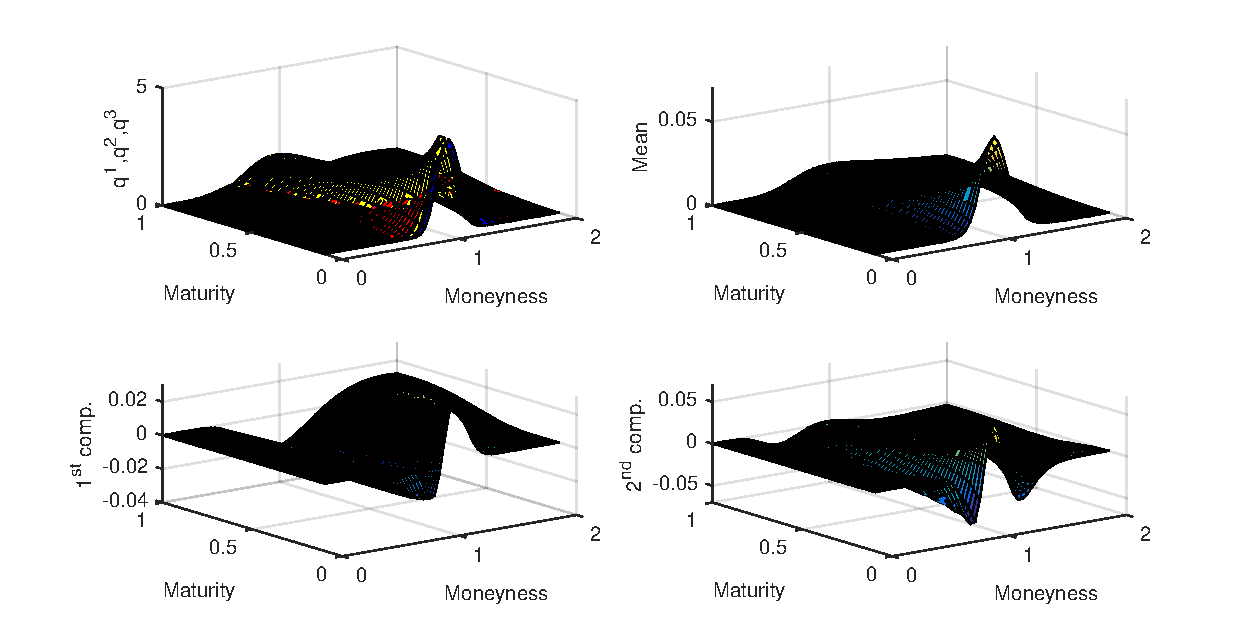
\includegraphics[width=1.00\textwidth]{Figures/Simulation2}
%\caption{\label{sim1} Simulated mixture components - log-normal densities $q^1$ - red; $q^2$ - blue; $q^3$ - yellow; Mean curve and orthonormal components}
%\end{center}
%\end{figure}


Without loss of generality, we set $r_{i\tau}=0$, for each day $i=i,\ldots,N$. %Then, in terms of the notations of section \ref{t2}, $X_i(m,\tau)=C_i(m,\tau)$ and $X_i^{(d)}(m,\tau)=q_i(m,\tau)$, for $d=(2,0)$. 
%The loadings are simulated from the positive half-standard normal distribution, then standardized to sum up to one. 
%Remember tat $r_{s,i}=\frac{s_i}{s_0}$. The stock price follows a geometric Brownian motion  with $\log(s_{i} / s_{i-1})\sim \mathbb{N}(0.03,0.18)$ for ordered time points $i=1,\ldots N$. The parameter choice corresponds to the empirical mean and variance of the stock index log-returns in the real data study. The starting value is $s_{0}=100$ and we fix the risk free rate to $0.02$ p.a. for all days. 
We construct a random grid for each observed curve $X_i$ by simulating points $t_{ik}=(m_{ik},\tau_{ik}), \; k=1,\dots,T$ from a uniform distribution with continuous support $[0.5,1.8]\times[0.2,0.7]$. %The first dimension is moneyness and the second maturity to match the features in the real data, see next subsection. 
%To get a coverage of the entire space like in the case of real data when few observations in the maturity direction are present 
%We additionally require that for ordered $\tau_l$, $\EE\left[\tau_l-\tau_{l+1}\right] = \frac{1}{3}$. 
Finally, we record noisy discrete observations of the call functions with the additive error term i.i.d. $\varepsilon_{ik} \sim \operatorname{N}(0,0.1^2)$.%, with $\sigma_{\varepsilon}=0.02$. 

%1. we know the shape of the orthogonal components 
%2. identification depends on the covariance of the loadings - in our example only two are identified - it depends on the sample covariance, depending on the signal to error ratio - can be viewed as error??? 
%3. implied volatility variation 
%By construction using a mixture of $L$ factors and $\sum_{l=1}^{L+1} w_{il}=1$ this model has $L-1$ principal components. 
%The simulated components $q_l$ and their orthogonal counterparts are shown in figure \ref{?}. 

%However, in our example, the third component is theoretically not identifiable. they are not always identifiable from the observations $q$ (or noisy versions of them). 


%The simulated components $q$ and their orthogonal counterparts are shown in figure \ref{?}. In our example $Var(w_1)=Var(w_2)=Var(w_3)=33\%$, while the variance of the orthogonal components are $97.97\%$, $1.77\%$ and $0.26\%$ respectively.

The true SPDs given by equation (\ref{trueSPD}) are used to verify the performance of $\hat{X}^{(d)}_{FPCA_1},\;  \hat{X}^{(d)}_{FPCA_2}$ and of the individually estimated curves $\hat{X}^{(d)}_{Indiv.}$, in terms of mean integrated squared error (MSE), i.e., $T^{-1} \sum_{k=1}^T \left\{X^{(d)}(t_{ik}) - \hat{X}^{(d)}_\bullet (t_{ik})\right\}^2$, for $d=(2,0)$. For evaluation we generate a common grid of 256 points from a uniform distribution.
%the mean squared error (MSE), which averages the errors for each curve  over number of curves time observations per curve. a discrete version of N^{-1} \sum_{i=1}^N 
To derive the optimal bandwidth in each case we stick to the rule-of-thumb approach presented in Section \ref{implementation}. %We adjust the rule to the given circumstance. 
The bandwidth for the individually smoothed curve $i$ is derived by replacing $\hat{p}^{(\nu)}_{ir}$ in (\ref{rulethumb}) by one and zero otherwise.
The performance is recorded for sample sizes $N$ of $10$ and $25$ with $T$ observations per day of size $50$ and $250$.  This procedure is repeated 500 times to get reliable results, mean, variance and the inter quartile distance based at the MSE of the repetitions are given in Table \ref{fig:SimuResults}. %to show how fast the asymptotics take effect
%To show that our bandwidth criteria works, we have experimented with 100 curves. We repeated the procedure 1000 times to show how fast the asymptotics take effect. 

 %In particular, for $b$ we have experimented with various bandwidths, e.g. we looked at the mean, minimum and maximum of individually optimal bandwidths. The best results are obtained for the maximum, hence, we report only these results in the following.
%Goodness of fit is measured in terms of the mean square error (MSE) per curve. We average the results for each repetition and report the sample performance using the average mean square error (AMSE). 
%Their effects are evaluated in the following simulation studies.
%We considered various simulation scenarios based on the combinations of the case of errors size and number of observation points and curves. 
%Tables \ref{table1} through \ref{table3} summarize the simulation results. %estimation results for curves estimated by FPCA and simple smoothing respectively. %For computing we use empirical centered true values. To guarantee a fair comparison we display AMSE for individual 


%smoothed curves as well with the optimal bandwidth for individual curves and in addition for the same level of smoothing like the FPCA (marked by *). %With a single exception FPCA performs better than its benchmark model. %The distribution of AMSE is synthetized in the boxlots from figure (\ref{boxplots}).
%We need to report how the optimal constant changes with the size of the noise. If there are differences then we'll get the constant equal to the our estimated $\sigma_{\varepsilon}$ in the real data example. 
%The results for the one repetition is summarized here: we find two factors because the third one is a linear function of the two. Make plot + ....
\begin{table}
\footnotesize
  \centering
  \begin{tabular}{c|c|c|c|c|c|c|c|c|c}
    \hline
    \hline
    &$T$&\multicolumn{4}{c|}{50}&\multicolumn{4}{c}{250}\\
    %\cline{3-6} 
		\hline
    $N$&$\hat{X}^{(d)}_\bullet$&Mean&Var&Med&IQR&Mean&Var&Med&IQR\\
    \hline
    \multirow{3}{12pt}{10}	&\footnotesize $FPCA_1$& 0.1876 & 0.0367 &0.1300 &0.1325& 0.0780 & 0.0025 &0.0643&0.0546\\
													&\footnotesize $FPCA_2$  & 0.2238 & 0.1212 &0.1295 &0.1466& 0.0762 & 0.0026 &0.0630&0.0518\\
													&\footnotesize $Indiv.$  & 0.2709 & 0.0900 &0.1928 &0.1838& 0.1105 & 0.0054 &0.0916&0.0708\\
								\hline
    \multirow{3}{12pt}{25}&\footnotesize $FPCA_1$& 0.0917 & 0.0066 &0.0680&0.0580& 0.0404&0.0006 & 0.0336 &0.0223\\
													&\footnotesize $FPCA_2$& 0.1553 & 0.0966 &0.0878&0.0887& 0.0586&0.0016 & 0.0489 &0.0406\\
													&\footnotesize $Indiv.$& 0.2691 & 0.0995 &0.1889&0.1848& 0.1111&0.0052 & 0.0916 &0.0719\\
    \hline  \hline
  \end{tabular}
  \caption{Results of the simulation described in Section \ref{simstudy} with different values for $T$ and $N$. $FPCA_1$ and $FPCA_2$ are superior in sense of MSE over the individual estimation of the derivatives in each setting. $FPCA_1$ is better than $FPCA_2$ except for $N=10$, $T=250$. For $FPCA_1$ and $FPCA_2$ the estimation improves with raising $N$ and $T$. These results support our asymptotic results given by Proposition \ref{Mbias} and \ref{curvebias}. }
  \label{fig:SimuResults}
\end{table}


%
%\begin{center}
%\textbf{[Insert Table~\ref{table1} approximately here.]} 
%\end{center}
%\begin{center}
%\textbf{[Insert Table~\ref{table2} approximately here.]} 
%\end{center}
%\begin{center}
%\textbf{[Insert Table~\ref{table3} approximately here.]} 
%\end{center}

Both FPCA based approaches gives better estimates for the derivative of the call functions than an individually applied local polynomial estimator of the individual curves. Both the mean and the median of the MSE are smaller which is a result of the additional average over $N$ for the basis functions as given by Proposition \ref{curvebias}. However, the $FPCA_1$ method performs decisively better for small $T$ than the other two both in terms of mean and standard deviation of the mean squared error. 
In addition  $FPCA_1$ benefits more from raising $N$ then $FPCA_2$. With small $T$ for $FPCA_2$ and individual smoothing the variability of MSE is much bigger than for $FPCA_1$ while the median of $FPCA_1$ and $FPCA_2$ are comparable. This means individual smoothing and $FPCA_2$  must behave much worse than $FPCA_1$ in some instances while $FPCA_1$ was able to stabilize the estimates. To get the same effect using $FPCA_2$ a much bigger $T$ is needed. A possible explanation for this behavior is given by Proposition \ref{Mbias}. The rates of convergence to estimate elements of the dual matrix solely rely on $T$ thus it is nearby that facing small $T$ some of the thereby derived loadings are inaccurate.
%For all estimation procedures the interquartile range (IQR) together with the standard deviation suggests that the distribution of MSE has fatter tails than normal and the comparison of mean and median also suggests a non normal distribution. %, in particular for the direct method. 

%Its performance depends on the sample characteristics and using it in applications has an associated higher risk. 
%In addition, the slow improvement in the direct method confirm that the order of convergence is dominated by the fixed number of observations per curve $T$. %the sample size of curves shall be very large to give comparable convergence with the indirect method. \color{red}Also possible that it never does, we need to increase the observation points. (Unless we increase the observation points ... it will never be asymptotically equivalent???) \color{black}


%Contrasting the interquartile range (IQR) with the standard deviation suggests that the distribution of MSE has fatter tails than normal, in particular for the direct method. 

%In particular, the direct method has many Looking at the IQR suggests that the large variance is due to the very bad performance of FPCA_2 in some of the cases (not necessarily outliers). The standard deviation stabilizes when we increase the number of curves (or not?). the small improvement in the fpca2 suggests that the number of curves shall be much higher. 




\subsection{Real Data Example }%\color{red}we only report results by our method\color{black}
\label{realData}
\subsubsection{Data description }We use daily settlement European call option prices written on the underlying DAX 30 stock index. The sample spans the period between January 2, 2002 and December 3, 2011 and includes a total of 2557 days. The option prices are computed at the end of the trading day by EUREX based on the recorded intraday transaction prices. %The data set was accessed through the Research Data Center (RDC) at the CRC 649. 
The expiration dates for the options are set on every third Friday of a month. Therefore, only option prices with a few maturities are available on a particular day, see Figure~\ref{exp}. The distance between two consecutive maturities is increasing with the maturity, while the distance between two consecutive strikes for the settlement option prices is relatively constant. This data structure, with only a few available maturities daily, still allow the use of local polynomial method for smoothing in our application because the estimates in the maturity direction can be interpreted as weighted averages of the neighboring estimates for fixed observed maturities. This is similar to interpolation that is often used in practice for option prices. %For this data structure containing sparse areas for high maturities, the nearest-neighbor interpolation method introduces potentially high bias since the call options are known to vary monotonically with the strike and the expiration date. Therefore, we choose instead the linear interpolation to get the curves on the common grid. In this setup, this gives better results in finite sample than the nearest neighborhood method. 
We include call options with maturity between one day and one year. Our sample contains prices of options with an average of six maturities and sixty-five strikes per day. % From these data we We don't use all these data because of truncations requited by finding the maximum overlapping domain over all curves.

We assume 'sticky' coordinates for the daily observations, see equation \eqref{q10}, and standardize both the strike and the call prices within one day by the forward stock index value to ensure that the observations are in the same range. %the observed options occur on the same range of relative strikes, that is our moneyness metrics $m$. %\color{red}Observations of each curve $C_i$ no longer occur at the same grid points. We use nearest neighborhood (in moneyness direction) and linear (in maturity direction) interpolation to compute the values of the call prices on an equidistant grid defined as the maximum common domain of observations in both dimensions. Our choice for the interpolation points is: thirty-one distinct grid points for the moneyness and twenty for the maturity. For simplicity, we treat them as direct observations further on. Consequently, we apply the FPCA to noisy standardized call prices and estimate their second derivative with respect to $m$ in a fixed design setup.\color{black}
%(The treatment of random design was already discussed in section.)%$T=[  \underset{t}{\left\{ \operatorname{max}} \left(\underset{j}{\operatorname{min}} R_{t,j}\right) \right\} ]x[]$.  
%In order to retrieve the estimated SPDs we also need risk free interest rate daily data for various maturities, see equation \eqref{q09}. We derive a proxy for these based on the term structure of the LIBOR rate. We compute the corresponding annual interest rate by linearly interpolating the available LIBOR rates on a daily base. 
%In the real data application we do not pre-multiply the daily observations with the corresponding $\exp{(r_{i,\tau},\tau)}$  in equation (\ref{q09}) and report the results of the FPCA decomposition in terms of equation (\ref{q}). %The implicit assumption is that for the considered time frame the risk free interest rate is constant. 
Following the methodological framework, we apply the FPCA to the rescaled call prices and report the decomposition results for their second derivative with respect to moneyness. %As a consequence, the estimated components have not been adjusted to account for the interest rate term structure in the maturity direction and its daily variability is incorporated in the loadings. To obtain the SPD on a particular day $i$ we need to multiply the second derivative of the call prices obtained from a reduced form model by $\exp{(r_{i,\tau}\tau)}$ for each maturity $\tau$, see equation (\ref{q09}). If one is interested in the SPD dynamics rather than in the call derivative, an alternative to this procedure is to pre-multiply the daily call observations by the corresponding discount factors
%$\exp{(r_{i,\tau},\tau)}$ 
%and afterwards apply FPCA to the adjusted prices. Each choice is best fitted to a particular research goal.
%For illustrating our framework and for the purpose of comparing our results with the empirical literature on the implied volatility surfaces we considered the first approach better suited. 
Our proxy for the risk-free
interest rates are the EURIBOR rates, which are listed daily for several maturities. We perform a linear interpolation to calculate the rate values for the desired maturities.% variation of the interest rate can be corrected for subsequently, if one is interested in the shape of the SPD on a particular. 
%This is achieved by considering daily yield term for discounting in the moneyness direction. 

%We do not pre-multiply the daily observations with the corresponding $\exp{(r_{i,\tau},\tau)}$  in equation (\ref{q09})


         
\begin{table}[ht]
\begin{center}
\begin{tabular}{c|r@{.}l  r@{.}l  r@{.}l  r@{.}l  r@{.}l  r@{.}l  r@{.}l  r@{.}l  r@{.}l  r@{.}l}\hline\hline      $r$,     $L_{\max}$ &\multicolumn{2}{c}{1}&\multicolumn{2}{c}{2}&\multicolumn{2}{c}{3}&\multicolumn{2}{c}{4}&\multicolumn{2}{c}{5}&\multicolumn{2}{c}{6}&\multicolumn{2}{c}{7}&\multicolumn{2}{c}{8}&\multicolumn{2}{c}{9}&\multicolumn{2}{c}{10}\\ \hline
  %\multicolumn{2}{c}{r=1}&\multicolumn{2}{c}{r=2}&\multicolumn{2}{c}{r=3}&\multicolumn{2}{c}{r=4}&\multicolumn{2}{c}{r=5}&\multicolumn{2}{c}{r=6}&\multicolumn{2}{c}{r=7}&\multicolumn{2}{c}{t=8}&\multicolumn{2}{c}{r=9}&\multicolumn{2}{c}{r10}\\ \hline
 $\lambda_r\times 10^{6}$&  133&29 & 18&90 &  2&69&  1&62 &  0&49 &  0&34 &  0&26  & 0&09 &  0&08  & 0&05\\
  % $\lambda_r\times 10^{6}$&  144&49 & 12&00 &  4&36 &  1&08  &  0&87 &  0&37 &  0&17  & 0&14 &  0&08  & 0&03\\
 % $\lambda_r^{(d)}\times 10^{6}$&   63&66 & 23&86 &  6&77 & 4&81 &  2&47 &   1&03  &  0&78  &  0&57  &  0&54  & 0&41\\  \hline
  $\lambda_r^{(d)}\times 10^{2}$&   14&74 & 3&76 &  2&83 & 2&14 &  1&12 &   0&80  &  0&20  &  0&19  &  0&515  & 0&12\\  \hline  
 % $\lambda_r /  \lambda_{r+1}$&   12&04  &  2&76  &  4&02  &  1&25 &  2&37 &  2&15 & 1&20  & 1&81  &  2&47 &  1&26\\
   $\lambda_r /  \lambda_{r+1}$&   7&05  &  7&01  &  1&66  &  3&28 &  1&44 &  1&31 & 2&83  & 1&18  &  1&70 &  1&35\\ 
 %$\lambda_r^{(d)} / \lambda_{r+1}^{(d)}$&  2&67  &  3&52 &  1&41 &  1&95  &  2&39  &  1&32  &  1&36  &  1&06 &  1&30  &  1&55\\    \hline
 $\lambda_r^{(d)} / \lambda_{r+1}^{(d)}$&  3&92  &  1&33&  1&32 &  1&92  &  1&40  &  4&01  &  1&04 &  1&23 &  1&27  &  1&37\\    \hline %$L$&\multicolumn{2}{c}{N/A}&\multicolumn{2}{c}{3}&\multicolumn{2}{c}{4}&\multicolumn{2}{c}{5}&\multicolumn{2}{c}{6}&\multicolumn{2}{c}{6}&\multicolumn{2}{c}{8}&\multicolumn{2}{c}{9}&\multicolumn{2}{c}{9}&\multicolumn{2}{c}{9}\\ 
 
%$k^*(PC^{(0)})$&\multicolumn{2}{c}{1}&\multicolumn{2}{c}{2}&\multicolumn{2}{c}{3}&\multicolumn{2}{c}{4}&\multicolumn{2}{c}{5}&\multicolumn{2}{c}{6}&\multicolumn{2}{c}{\textbf{7}}&\multicolumn{2}{c}{\textbf{8}}&\multicolumn{2}{c}{\textbf{9}}&\multicolumn{2}{c}{9}\\  
$k^*(PC^{(0)})$&\multicolumn{2}{c}{-}&\multicolumn{2}{c}{-}&\multicolumn{2}{c}{-}&\multicolumn{2}{c}{-}&\multicolumn{2}{c}{-}&\multicolumn{2}{c}{-}&\multicolumn{2}{c}{7}&\multicolumn{2}{c}{8}&\multicolumn{2}{c}{9}&\multicolumn{2}{c}{9}\\ 
   
%$L_d$&\multicolumn{2}{c}{N/A}&\multicolumn{2}{c}{3}&\multicolumn{2}{c}{4}&\multicolumn{2}{c}{5}&\multicolumn{2}{c}{5}&\multicolumn{2}{c}{5}&\multicolumn{2}{c}{6}&\multicolumn{2}{c}{7}&\multicolumn{2}{c}{9}&\multicolumn{2}{c}{10}\\ 

$k^*(PC^{(d)})$&\multicolumn{2}{c}{-}&\multicolumn{2}{c}{-}&\multicolumn{2}{c}{-}&\multicolumn{2}{c}{-}&\multicolumn{2}{c}{-}&\multicolumn{2}{c}{-}&\multicolumn{2}{c}{6}&\multicolumn{2}{c}{8}&\multicolumn{2}{c}{9}&\multicolumn{2}{c}{10}\\ 
%$k^*(PC^{(d)})$&\multicolumn{2}{c}{1}&\multicolumn{2}{c}{2}&\multicolumn{2}{c}{3}&\multicolumn{2}{c}{4}&\multicolumn{2}{c}{5}&\multicolumn{2}{c}{\textbf{6}}&\multicolumn{2}{c}{6}&\multicolumn{2}{c}{\textbf{8}}&\multicolumn{2}{c}{\textbf{9}}&\multicolumn{2}{c}{\textbf{10}}\\ 
% $k^*(PC^{(d)})$&\multicolumn{2}{c}{1}&\multicolumn{2}{c}{2}&\multicolumn{2}{c}{3}&\multicolumn{2}{c}{4}&\multicolumn{2}{c}{5}&\multicolumn{2}{c}{5}&\multicolumn{2}{c}{6}&\multicolumn{2}{c}{7}&\multicolumn{2}{c}{9}&\multicolumn{2}{c}{10}\\ 
%\hline
%$r'$&\multicolumn{2}{c}{1}&\multicolumn{2}{c}{2}&\multicolumn{2}{c}{7}&\multicolumn{2}{c}{6}&\multicolumn{2}{c}{8}&\multicolumn{2}{c}{3}&\multicolumn{2}{c}{9}&\multicolumn{2}{c}{5}&\multicolumn{2}{c}{4}&\multicolumn{2}{c}{15}\\ 
\hline\hline
    \end{tabular}
\caption{\label{baing} Estimated eigenvalues and eigenvalue ratios. Number of factors by $PC^{(\nu)}$ criteria.} %Index of sorted component $\hat{\gamma}_{r,T}$ in decreasing order for explained variance}
\end{center}
\end{table}
\subsubsection{Estimation results } %The implementation of criteria (\ref{optk}) for the choice of $L$ and $L_d$ suggests a three factors for the call option surfaces dynamics, and two-factors for the dynamics of state price density surfaces, see also figure \ref{basis}. The first three and two respectively largest eigenvalues explain a disproportionate amount of variance compared to the subsequent ones, which are all close to zero. %, depending on the choice of $K_{\max}$. 
%The implementation of criteria (\ref{optk}) for the choice of $L$ suggests at least three and for $L_d$ two components. The corresponding largest eigenvalues of the covariance operators for the call option and state price density surfaces are much larger then the subsequent ones, which are either close to zero or approach zero after a few other components (figure \ref{?}). This implies that we can use a factor model as in (\ref{approx11}) to represent the dynamics of state price density surfaces. Since the theoretical and simulation results recommend using the decomposition (\ref{der2}) over (\ref{pder2}) for estimating derivatives, we report the results obtained by the estimation and eigendecomposition of $M^{(0)}$. The error surface ....
The first eigenvalue of the dual covariance matrix $\hat{M}^{0}$ for the call option surfaces has a dominantly strong explanatory power and the order of magnitude of the following eigenvalues decreases by a factor of ten with every few additional components.
%starting with the third component the eigenvalues have the same order of magnitude. %the following components decay fast.
%, see Table \ref{baing}. % and approach zero after a few other components \color{red}(test for lambda=0)\color{black}. 
Following \cite{Ahn2013}, we also construct the eigenvalue ratio of two consecutive eigenvalues in descending order. The first two terms in the sequence are relatively high and there are a few other increasing terms, e.g., the fourth, seventh and ninth, before the sequence decreases towards one. %approaches one from above. %stabilizes close to one. %The largest value of this ratio - if we ignore the first component - gives three components, and the ratio stabilizes around one only after the ninth component.
%The evaluation of the information criterion of \cite{Bai2002}, see equation (\ref{optk}) for the choice of $L$, has a minimum at $k=3$ for $L_{max}=2$. Further evaluations of the criterion suggest up to eleven components.  We report the case $L=3$, which is an upper bound for $L_d$. We also discuss subsequently the effect of including additional factors on the stability of results. 
The choice of the maximum number of factors by the $CP^{(0)}$ criteria suggests at least seven components. This can be seen by looking at the values of $k^*$ for $L_{max}\geq 7$ in Table \ref{baing}. %, which are independent of the constrain $k\leq L_{max}$ in the objective function (\ref{optk}). %and its unconstrained equivalent ($k \in \mathbb{N}$) are identical for $L_{max}\geq 7$, marked bold in Table \ref{baing}. %, (it is minimized at $L_{\max}$ for $L_{\max} \leq 6$).  
$IC^{(0)}$ criterion, which does not depend on the truncation parameter $L_{max}$, gives seven components. %We report below the upper bound case $L_d\leq 7$.
%case $L=7$, which is an upper bound for $L_d$.% We also discuss subsequently the effect of including additional factors on the stability of results. % hereafter a parsimonious factor model with
%This implies an upper bound on $L_d$ of maximum three components. 
\begin{figure}[ht]
\begin{center}
%\includegraphics[width=1.00\textwidth]{figures/Callssecondloadings75} \\
%\includegraphics[width=1.00\textwidth]{figures/Callssecondloadings76} 
\includegraphics[width=1.00\textwidth]{Figures/CallsloadingsNEWforward1392}
%\caption{\label{second_comp} Left: Call options on the expiration day. Right: Second non-orthogonal component $\hat{\gamma}_{2,T}$}
\caption{\label{exp} The effect of the expiration date on $\hat{\delta}_{2,T}$}
\end{center}
\end{figure}

A closer look at the dynamics of the loadings, shows an unusual behavior of some of them - $\hat{\delta}_{2,T}$, $\hat{\delta}_{4,T}$, $\hat{\delta}_{5,T}$ and $\hat{\delta}_{6,T}$ - between mid-February 2007 through mid-June 2008. This interval spans the period before the beginning of the financial crisis and extends to the end of the recession in the Euro Area - according to the Center for Economic and Policy Research (CEPR) recession indicator. %It shows a recession from the period following the peak through the trough - 
The loadings are extremely volatile and display a certain time regularity of jumps. We identified these jumps with the Mondays following an expiration date - which occurs on a single Friday in every month, see Figure \ref{exp} that links the dynamics of $\hat{\delta}_{2,T}$ to the expiration days. After the sudden decrease, the loadings increase day-by day and approach a 'normal' level after about two weeks. %, as the string of options with the smallest available maturity approaches expiration. 
%During this period, the call prices for small maturities are extremely convex at-the-money and the absence of a call string with close enough small maturity on the following trading Monday leads to severe bias in the values of $\hat{C}^{(\nu)}_{i,b}(m,\tau)$, estimated through equation (\ref{polyeqkern}), for $\tau<\min(\tau_i)$. 

\begin{figure}[ht]
\begin{center}
%\includegraphics[width=1.0\textwidth]{figures/Nonorthogonalbasis20160502} 
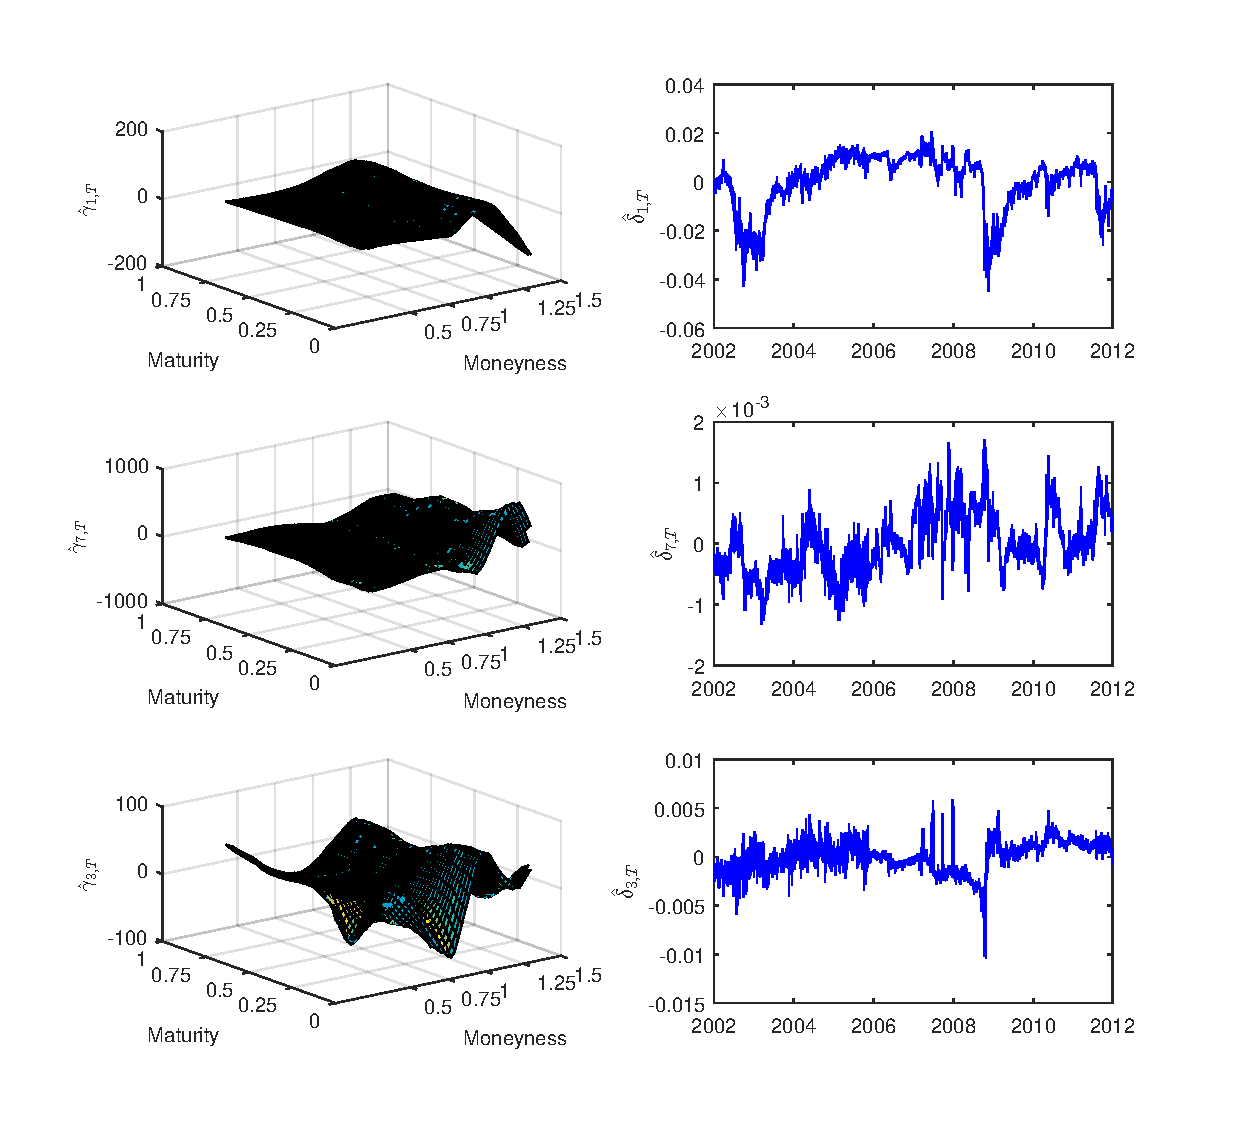
\includegraphics[width=1.0\textwidth]{figures/Nonorthogonalbasis20160521}
%\includegraphics[width=1.00\textwidth]{figures/Nonorthogonalbasis1} \\
%\includegraphics[width=1.00\textwidth]{figures/LoadingsFPCA1}
%\includegraphics[width=1.00\textwidth]{figures/Nonorthogonalbasis2} 
%\caption{\label{second_comp} Left: Call options on the expiration day. Right: Second non-orthogonal component $\hat{\gamma}_{2,T}$}
\caption{\label{nonort} Estimated non-orthogonal components and their loadings obtained by the decomposition of $\hat{M}^{(0)}$, in decreasing order of explained variance from up to bottom}
\end{center}
\end{figure}


During this period, there are not many observations available for the call prices with strikes larger than the current stock index price for small maturities. Together with the absence of a call string with close enough maturity on the following trading Monday, this introduces bias in the smooth estimated call surface, for grid values outside the range of observation points. %, stemming from the extrapolation problem for the local kernel regressions. 
However, we cannot rule out the possibility that the importance of the second component is not due to an error in pre-smoothing of the call options used for the estimation of $M^{(0)}$ because even if we recalculate the explained variance for all the components after excluding the estimated loadings from this time interval, this factor still remains the second most important. The shape of the second estimated component $\hat{\gamma}_{2,T}$, displayed in Figure \ref{exp}, suggests that it is related to the short end of the SPD term structure effect. The other components $\hat{\gamma}_{4,T}$, $\hat{\gamma}_{5,T}$, $\hat{\gamma}_{6,T}$ and $\hat{\gamma}_{8,T}$, whose loadings have similar behavior, are similar in shape to the four components we have discussed so far, i.e., $\hat{\gamma}_{1,T}$, $\hat{\gamma}_{2,T}$, $\hat{\gamma}_{3,T}$ and $\hat{\gamma}_{7,T}$. It is yet not totally clear but it is well possible that they are related to the asymmetric behavior of the option prices along the maturity direction, i.e., the term structure effect of the SPDs. %- more than one factor is necessary to explain the variation in the time to maturity direction. %We therefore focus on the remaining three components. %The evidence indicate is an indicative that the importance of the second component is due to an error in pre-smoothing of the call options used for the estimation of $M^{(0)}$, and we exclude it from our further analysis. Note that even if we recalculate the explained variances for all the components after removing the loadings from this time interval, this factor still remains important, \color{red}which may imply that the smoothing error affects the results for our entire sample \color{black}. Further, we look at the shape of the other components and the dynamics of their corresponding loadings. The loadings of components $\hat{\gamma}_{4,T}$, $\hat{\gamma}_{5,T}$ and $\hat{\gamma}_{6,T}$ suffer from the same problem as $\hat{\delta}_{2,T}$. We therefore remove them from the candidate factors. \color{red} ???? they are related to short term effects. \color{black}

%Further $\hat{\gamma}_{4,T}$ and $\hat{\gamma}_{7,T}$ are similar in shape to $\hat{\gamma}_{2,T}$ and


%We further report on the other the case $L=3$, which is an upper bound for $L_d$. We also discuss subsequently the effect of including additional factors on the stability of results. For visualization, we multiply the estimated components by the standard deviation of the corresponding loadings. 
%\begin{figure}[ht]
%\begin{center}
%\includegraphics[width=1.00\textwidth]{figures/phi6}  
%\caption{\label{ort} First six orthogonal components obtained by the decomposition of $\hat{M}^{(0)}$}
%\includegraphics[width=1.00\textwidth]{figures/phi}  
%\caption{\label{ort} First eight orthogonal components obtained by the decomposition of $\hat{M}^{(0)}$}
%\end{center}
%\end{figure}




%The other three most important estimated non-orthogonal components 
The remaining three estimated components are displayed in Figure \ref{nonort}, in order of their explained variance, see equation (\ref{varnno}). %To enable comparison, they have been multiplied by the standard deviation of the corresponding loadings. %Scaled $\hat{\gamma}_{1,T}$ and $\hat{\gamma}_{3,T}$ are similar in hight but the peak of 
%The first component is aligned with the mean, and has positive values around the peak and negative around the tails. The other two components resemble the orthogonal components in the simulation study. Some differences stem from the fact that the empirical SPD are left-skewed, compared to the right-skewed mixtures of log-normals. %This also explains a lower first 'valley' in the second component. Another difference in the tail behavior of the first two components - steep slope and negative values - might be due to interpolation errors in the regions with few observations. Other than that, the components provide a similar interpretation to those in the simulation study. 
These three components describe three types of asymmetry present in the dynamics of the SPDs. Their interpretation, is linked to the shape of the empirical mean of the SPD, which has a long tail on the left side of the peak. %A negative skew reflects the market expectation that the future stock index will be above its forward value. While negative skewness risk can bear excess returns, during periods of economic downturn, the investors prefer positively skewed distributions. 
The first component has positive values around the peak and negative around the tails and is related to the volatility dynamics. An increase in the loadings of this component decreases the volatility of SPD. The second component has a lean 'valley' at the left of the sample mean, which takes negative values, and a more pronounced 'hill' at the right, which feature positive values. This component emphasized the dynamics of negative skewness and induces as well changes in the kurtosis of the density. % mass around the mean of the distribution and can 
We interpret it as the negative skewness factor. The third component has a more symmetric 'valley-hill' pattern, which shifts mass around the central region of the density. It also influences the density far left tail. A positive shock in the direction of this components increases the negative skewness, while a large enough negative shock will render the SPD positively skew. This component is interpreted as the sign of skewness factor.  % and influences also particularly the the to the tails at the expense of the regions in between in a disproportionate fashion. The variations are larger in amplitude in the left half of the distribution. This component is interpreted as a kurtosis factor. 
%crosses zero four times (for fix maturity). It influences the kurtosis of the density: it %simulated that of the second component is shifted to the right and is steeper for maturities of less than three months - options with shorter maturities are supposed to react stronger to changes. Both their right tails are negative, possibly due to the smoothing errors outside the observable data region. 


%The loadings $\hat{\delta}_{1,T}$, $\hat{\delta}_{7,T}$  and $\hat{\delta}_{3,T}$ display a time-varying volatility regime, which divide the sample in three sub-periods that may reflect the impact of the global environment on the option prices. The end of 2005 marks the decline in the global liquidity and the end of 2008 is the conjectured conclusion of the global financial crises. Formal statistical tests for the equality of the loadings variance within the three subperiods can be run for a more thorough analysis. This can possibly unveil interesting economic questions, which will have to be left for further research. %We do not follow up on these observations because, as we show in the following, this variation is not longer present after orthogonalizing the loadings. %  \color{red}Changes in the mixture's distribution? We can interpret these as possibly changes in the mean function of the call prices or changes in the underlaying components Irina cite paper\color{black}. We will look at this issue in our following analysis. We will briefly return to them when discussing the connection between the SPDs and VDAX, in section \ref{?}. 
%Therefore, we delete components two and four to represent the dynamics of $\bar{C}^{((2,0))}$ in terms of the orthogonal components, see figure \ref{rez}. 


%From the simulation study we know that the variation explained by the third orthogonal component for density mixtures is significantly smaller than those of the first two. This is likely to translate in relatively small variations of the call prices as well. However, this component is important for explaining the moments of the DAX returns, for hedging or pricing purposes. We are therefore interested to identify it from the noisy data. Based on the criteria for the choice of number of factors, a less conservative choice for a proper truncation of the model is $L=9$. 

% If we exclude this period from our sample the forth component is not 'loosing' its importance as well.
 %Here, it proves useful to have some prior knowledge about the shape of the components we expect to identify empirically.
%When investigating the variation of densities, one must be cautions because - as seem in the simulation study - the variation explained by further components is relatively small compared to the first two ones. Hence, without a proper ``shape marker/identifier'' one might easily confound them with noise. 
 %It proved useful to have some prior knowledge about the shape of the orthogonal components in order to choose a proper truncation of the model. 
%First, we look at the shape of the components and the dynamics of their corresponding loadings. Components $\hat{\gamma}_{4,T}$ and $\hat{\gamma}_{7,T}$ are similar in shape to $\hat{\gamma}_{2,T}$ and their loadings suffer from the same problem as $\hat{\delta}_{2,T}$. We therefore remove them from the candidate factors.

%\begin{figure}[ht]
%\begin{center}
%\includegraphics[width=1.00\textwidth]{figures/Rotatedorthogonal1} \\
%\includegraphics[width=1.00\textwidth]{figures/Rotatedorthogonal2} 
%\includegraphics[width=1.00\textwidth]{figures/Orthogonalbasis1mew}\\
%\includegraphics[width=1.00\textwidth]{figures/Orthogonalbasis2mew}
%\caption{\label{second_comp} Left: Call options on the expiration day. Right: Second non-orthogonal component $\hat{\gamma}_{2,T}$}
%\caption{\label{nonortrot} First four rotated orthogonal components when including  $\hat{\gamma}_{1,T}$, $\hat{\gamma}_{2,T}$ and$\hat{\gamma}_{3,T}$}
%\end{center}
%\end{figure}

% The purely autoregressive model explains the dynamics of the risk-neutral implied moments rather well. \color{red} Adding exogenous variables to the vector autoregression does not improve the explanatory power of our model. \color{black} 
 
 
 

%One-step ahead forecasting accuracy, measured as the RMSE of the in-sample forecasting errors imply that the first model is better in terms of prediction. These models can be used to investigate Granger causality relations between the loadings. 



%The shape features of the three components from Figure (\ref{nonort}) and their ordering according to the explained variance are stable to orthogonalization, when we use the truncation choice  $\sum_{r\in \{1,3,7\}}\hat{\delta}_{r,T}\hat{\gamma}_{r,T}$. 
The functional principal components for the reduced model $\sum_{r\in \{1,3,7\}}\hat{\delta}_{r,T}\hat{\gamma}_{r,T}$ resemble closely the three components from Figure \ref{nonort}. % is possibly introduced through the dynamics of the interest rate term structure
%This means that if we ignore the term effect, which expresses the asymmetric reaction intensity to changes in the economic environment between the short and long term term option prices, the first three orthogonal components of the reduced model can still be interpreted as volatility, skewness and kurtosis factors. To avoid the burden of introducing additional notation we use non-orthogonal estimates in our further analysis. 
Further analysis shows that if we add any of the term structure components, whose loading feature a behavior similar to $\hat{\delta}_{2,T}$, with their inherent jump before, the shape of the components changes slightly. In addition, the loadings of all orthogonalized components are 'contaminated' with jumps. %Therefore, we use only three basis to describe the dynamics of SPDs % if the term structure effect of the SPDs is not considered. Variations of SPD in the maturity dimension introduces additional components, which are required to describe the asymmetric SPD changes for short and long maturities, similarly to the main modes of variation in the reduced model. %to reflect the uneven changes introduced by the term structure variation. %around the mean, skewness and kurtosis.
In fact, all the loadings of the estimated components (not displayed here) by decomposing $\hat{M}^{(d)}$, for $d=(2,0)$ display the jump-behavior we described before between mid-February 2007 and mid-September 2008. In that sense, the previous approach seems to provide more accurate estimates that allow for a better interpretation of the results.
%We verified this by varying the number of factors before orthogonalization. We found that the shape features of the first three orthogonalized components from is preserved, while their loadings display jumps, similarly to $\hat{\delta}^{(d)}_{2,T}$ if any of the other 'noisy' components are added, similarly to the loadings $\hat{\delta}^{(d)}_{r,T}$. In fact, shape-wise $\hat{\gamma}_{1,T}$, $\hat{\gamma}_{2,T}$ and$\hat{\gamma}_{3,T}$ correspond to the estimates $\hat{\varphi}_1^{(d)$, $\hat{\varphi}_2^{(d)$ and $\hat{\varphi}_1^{(d)$. The other three orthogonal basis obtained from the decomposition of $\hat{M}^{(d)}$, are also related to the behavior of short term maturities. For instance, $\hat{\gamma}_2^{(d)$, closely resemble $\hat{\varphi}_4^{(d)$. We posit that three basis are necessary to explain variation of the SPDs if the term effect is not considered. The term effect introduces additional components, that decompose the term variation in variation around the mean, skewness and kurtosis. %The correlation structure between the loadings $\hat{\delta}_{r,T}$ and $\hat{\delta}^{(d)}_{r,T}$ are showed in table \ref{????}.

%Further, we analyze our results in terms of the orthogonal components. This allows us to perform a direct comparison between the estimation of the SPD by the two methods we presented in the previous sections. %compare them with the alternative estimation method based on the decomposition of $\hat{M}^{(d)}$. 
%For this, we rotate the remaining six components, by applying a projection $a$, such that: $\sum_{r\in \{1,3,5,6,8,9\}}\hat{\delta}_{r,T}\hat{\gamma}_{r,T}=\sum_{r=1}^6a_r \tilde{\varphi}_r^{(d)}$, where $\tilde{\varphi}_r$ are the functional principal
%components for the reduced model and $a_r$ the corresponding loadings. By proceeding in  this way, the important commonalities in the nonorthogonal factors will be concentrated in even fewer components. %This also allows us to interpret our results in terms of components with known shape and also compare them with the alternative estimation method based on the decomposition of $\hat{M}^{(d)}$. 
%The results are displayed in figure \ref{nonortrot}, for the first four orthogonalized components. The first three closely resemble the orthogonal components from our simulation study. One difference stems from the fact that the empirical SPD are left-skewed, compared to the right-skewed log-normals and their mixtures. This also explains a lower first 'valley' in the second component. Another difference in the tail behavior of the first two components - steep slope and negative values - might be due to interpolation errors in the regions with few observations. Other than that, the components provide a similar interpretation to those in the simulation study. They describe three type of asymmetries present in the dynamics of the SPDs. The first component that peaks at the same location as the mean curve, redistributes mass from the peak to the tails and can be related to the volatility dynamics. The second component, can be interpreted as influencing the skewness of the density: it adds mass to the central region and subtracts mass from the tails. The third component, shifts the density mass between the left and right sides and can be linked to the skewness factor. The corresponding loadings $a_r$ are no longer appear to be heteroskedastic. We will return to the analysis of their dynamics in the next subsection. (short characterization of the dynamics that anticipate findings in the next section).


%Two orthonormal components explain almost the entire variance of the reduced model, namely $99.74\%$ and $0.26\%$ respectively. 3rd??? The role played by the two components in explaining the variation of the SPD must be interpreted with caution, as changes in different regions of the underlying density may signal changes in the characteristics of underlying economic risks and market reaction to them, as well as impact the prices of the contingent clams on the underlying asset in a disproportionate fashion. For instance, it is well known that the deformation of the tail distribution conveys important information about the probability of extreme events that affect portfolio performance and hedging decisions. For the European options, small changes in the small probabilities can affect substantially the prices of far out of the money (OTM) options. Our further ananlysis suggests that both components are essential in undertanding the dynamics of SPD. Pricing of OTM Puts and Calls - asymmetris in the 

%The second orthonormal component presents a positive peak situated around the peak of the mean. The right tail displays more negative values whereas the values of the component in the left tail fluctuate around zero negative. A positive shock in the direction of this component increases the peakness of SDP over the mean and decreases the mass of the distribution in the tails, in particular in the right one. 

%\color{red}How do the factors influence the option prices?\color{black} Changes in the shape of the SPD translate to changes in the option prices. Whenever the probability mass for certain values of moneyness increases it will result in higher weights associated to the payoffs of the option in that particular states. For instance, a positive shock in both components will result in more expensive medium range OTM and cheaper far OTM calls. Conversely, a negative shock will make the prices of both far OTM put and call options increase while the prices of medium range OTM calls will decrease. This behavior can be related to the hedging behavior on the option market, see the discussions in \cite{Bollen:04}, \cite{Constantinides:11} and \cite{Kra:15}. % explain this behavior by  they don't like uncertainty. 



%that including additional components preservesthe explained variance increases with each with each component that we include in the reduced model.


%We verified the consistence of our results by varying the number of factors before orthogonalization. We started by including only two components, $\hat{\gamma}_{1,T}$ and $\hat{\gamma}_{3,T}$, and investigated the principal components and their loadings for the reduced model. We repeated the procedure by increasing the number of components one at a time. We found that including additional components preserves the features of the first two orthogonalized components from figure \ref{nonortrot}, while the explained variance increases with each with each component that we include in the reduced model. The shape of the third component becomes stable once we add $\hat{\gamma}_{6,T}$. If we include only three components ($\hat{\gamma}_{5,T}$) then the third principal component is similar in shape to the fourth component in figure \ref{nonortrot}. Finally, deciding how large $L_d$ should be taken in practice, i.e. how many principal components, is both a matter of interpretation ability in terms of the shape of the components and of their loadings to capture as much variance in the data as possible, and adequately describe the dynamics of the underlying high-dimensional curves by correctly eliminating the noise terms.  \color{red} approximate factor model ???\color{black}



%The loadings are strongly correlated. This means that a factor model may be appropriate.
%This observation is supported by the results from the decomposition of $\hat{M}^{(d)}$, for $d=(2,0)$. Most of the criteria for choosing $L_d$ by this approach suggest six components. 

%The optimal choice for $L_d$ from the $CP^{(d)}$ criteria gives at least six components, while both the eigenvalue ratio and $IC^{(d)}$ give six components. If we look at Figure \ref{ort}, we notice that there are three pairs of similarly-shaped components: the first pair $\hat{\varphi}^{(d)}_{1,T}$ and $\hat{\varphi}^{(d)}_{2,T}$ relate mainly to changes in the volatility, the second pair $\hat{\varphi}^{(d)}_{3,T}$ and $\hat{\varphi}^{(d)}_{5,T}$ looks similar to $\hat{\gamma}^{(d)}_{2,T}$, while the third pair $\hat{\varphi}^{(d)}_{4,T}$ and $\hat{\varphi}^{(d)}_{6,T}$ is similarly shaped to the negative skewness component from the previous decomposition. %The first pair relate to the volatility, the second pair appear similar to $\hat{\gamma}^{(d)}_{2,T}$, while the third pair is similar to the negative skewness factor. %However, this interpretation is not straight-forward and investigating additional components might shed additional light into this issue. 


%We plot as well $\hat{\varphi}^{(d)}_{7,T}$ and $\hat{\varphi}^{(d)}_{8,T}$, which can be interpreted as skewness sign factors. These components are quite small and some of the criteria for the selection of the number of factors based on this approach might be overlooking his importance. Except for the first components estimated by each method, the loadings corresponding to $\hat{\varphi}^{(d)}$ and $\hat{\gamma}^{(d)}$ display only mild or low correlations. Therefore, a direct correspondence between the components is not straight forward. However, an approximate factor model is possible to hold for these data. As regards the 'duplicity' of the components, our results are most likely a manifestation of the SPD term effect, e.g. options with various maturities react differently to changes in the economic conditions. Accordingly, two factors in the term structure dynamics imply that two sets of components are required to explain the SPD implied expectations of long and short-run moments. This assumption is supported by looking particularly at the shape of the first pair, where the first component is relatively flat and describes reactions in the SPDs for longer horizons and the second component is steeper and describes reactions in the SPDs for short maturities.%.  we contend that the two sets of components describe reactions in the SPDs for long and short maturities. %as clear as in the case of $\hat{\gamma}^{(d)}_{r,T}$s.  
%Not displayed here, all the loadings of the estimated components by decomposing $\hat{M}^{(d)}$ display the jump-behavior we described before between mid-February 2007 and mid-September 2008. In that sense, the previous approach seems to provide more accurate estimates that allow for a better interpretation of the results. %These results occur because the extrapolating error is worse for the second derivative. They are, however, stable in terms of the volatility of the loadings. 
%Approximate factor model might be possible if we look at figure \ref{ort}.

%The estimated correlations between $\hat{\delta}_{r,T}$ and $\hat{\delta}^{(d)}_{r,T}$ displayed in table \ref{corrt} show a strong correlation only between the loadings of the first components estimated by each method, while the other correlations are quite small. No significant correlations are obtained after applying FPCA to the reduced model either. (Try 8 components). The results are thus mixed, if a factor model is appropriate for our data. (Maximum correlation - maximize correlation between projections - Markus paper).

%From the simulation, we have learned that the variance explained by each additional components decreases 'more than' exponentially for each additional factor added, when there is no term structure effect. This is why, when decomposing the variance explained ... 1.2550     0.0025      0.0001 multiplied by a factor of $10^7$. In Table 2 - Reordered variance. How to decide on the number of factors? 


%The optimal choice for $L_d$ from the $CP^{(d)}$ criteria gives $L_{\max}$ components for $L_{\max} \leq 5$, while $IC^{(d)}$ gives six components. The forth component is obviously related to the short-term maturity effect. In general, the loadings of all estimated components by decomposing $M^{(d)}$ display the jump-behavior we described before between mid-February 2007 and mid-September 2008. These results occur because the extrapolating error is worse for the second derivative.They are, however, stable in terms of the volatility of the loadings. 

% for the dynamics of state price density surfaces.
%The first two estimated principal components are similar to the functional principal components of the reduced model, see figure \ref{ort}. The pairwise correlation between their corresponding loadings is also high, $corr(\hat{\delta}^{(d)}_{1,T},a_1)=0.75$ and $corr(\hat{\delta}^{(d)}_{2,T}a_2)=0.73$. The third component does not offer conclusive evidence either with respect to the shape or the correlation $corr(\hat{\delta}^{(d)}_{1,T},a_1)=-0.23$, which is relatively small. The forth component is obviously related to the short-term maturity effect. In general, the loadings of all estimated components by decomposing $M^{(d)}$ display the jump-behavior we described before between mid-February 2007 and mid-September 2008. %Further components are also relatively smooth compared to $\tilde{\phi}_4^{(d)}$ and they seem also affected by the small-maturities effect. 
%These results occur because the extrapolating error is worse for the second derivative. % it might be that the second derivative amplifies the noise. One problem that occurs when taking derivatives is 
%They are, however, stable in terms of the volatility of the loadings. 
%A factor model with two components based on equation 
%we choose the number of factors to be = to the largest variance before the reordering 

 \begin{figure}[ht]
\begin{center}
\includegraphics[width=1.00\textwidth]{figures/ACPAC}  
\caption{\label{acpac} Autocorrelation (AC) and partial autocorrelation (PAC) of the estimated loadings and of their difference}
\end{center}
\end{figure}

\subsubsection{Dynamic analysis of the loadings }
We look at the dynamics of the SPD as summarized by the reduced model. By construction, the loadings are orthogonal, however their movements suggest strong dependencie. A negative skewness of the SPD reflects the market expectation that the future stock index will be above its forward value. Usually, the negative skew increases together with the implied volatility. While negative skewness risk can bear excess returns, during periods of economic downturn, the investors prefer positively skewed distributions. This can be seen when looking at the large negative values of $\hat{\delta}_{3,T}$ which, in effect, shift the SPD mass from the positive to the negative side of the distribution, in conformity with an increase in the risk aversion of investors.

In the following, we would like to understand how past realizations of the loadings influence present observations. 
%How past values of Ds influence future values. 
Figure \ref{acpac} displays the sample autocorrelation and partial autocorrelation
functions for the loadings from Figure \ref{nonort} and their first difference. Autocorrelation functions of the loadings decay very slowly suggesting nonstationarity in the time series. Standard tests for the presence of unit roots are performed for the loadings provide evidence of unit-root in the level of the loadings. Engle-Granger and Johansen tests for pairwise and multiple cointegration relationship between the loadings indicate that the series are cointegrated.


After taking the first difference the high persistence vanishes and there is a single significant spike for the first lag.
The partial autocorrelation functions for the first difference spike at the first lag and decreases over the next few lags.
%slowly for the next three-four lags. 
The results suggest that an ARIMA(1,1,1) %or ARIMA(4,1,1)
model might be appropriate to model the loadings. Its continuous-time equivalent, the mean-reversion process, has been used to model the changes in the implied volatility surfaces, see \cite{Cont:02}. In the following, we focus on the discrete time model and use a vector-autoregressive model (VAR) for the first difference of the loadings. 
\[
y_i=\Omega y_{i-1}+\varepsilon^{\footnotesize{VAR}}_i,
\]
where $y_i=(\Delta \hat{\delta}_{i1} \mbox{ } \Delta \hat{\delta}_{i3} \mbox{ } \Delta \hat{\delta}_{i7})^{\top}$, for $\Delta \hat{\delta}_{ir} =(\hat{\delta}_{ir,T}-\hat{\delta}_{i-1 r,T})$, and $\Omega$ is a coefficient matrix. The results of the estimation procedure are presented in Table \ref{tab1}. This model specification also allows us to employ a Granger causality test to assess whether the loadings of one component is actually useful in predicting the future levels of the other SPD components. The results of the test, summarized in Table \ref{tab2} show that daily changes in the negative skewness factor are not caused by the changes in the volatility factor. The other variables Granger-cause each other. \color{red}Also notice that we have tested for Granger Causality for multiple lags and the results are quite robust. \color{black}%\color{red}loadings are integrated. Also verify this for different Lag size - up to three months: Need to redo it but it seems that d3 cannot be predicted. also, from one to four weeks it can be predicted.  \color{black}


\begin{table}\label{granga}
\footnotesize 
\begin{center}
%\begin{center}
\begin{subtable}{.5\linewidth}
\begin{tabular}[t]{c|c|c|c|c}
\hline \hline
\footnotesize $\Omega_{i,j}$ & $j=1$ & $j=2$ & $j=3$& a. $R^2$\\
\hline
\footnotesize $i=1$ &    $-8.84^{**}$    & $58.59^{***}$   &  $91.05^{**} $  &  0.1328\\
\footnotesize $i=2$  & $ 3.96^{**} $  & $-32.90^{***}$   &$ -35.58^{**} $ &  0.2012\\
\footnotesize $i=3$ &   $0.22$ &  $-2.51^{***} $  & $-28.90^{***}$  & 0.1589 \\
%\hline
%a. $R^2$ &  0.1328 &  0.2012 & 0.1589 \\
\hline \hline
\end{tabular} 
     \caption{\label{tab1} \footnotesize VAR coefficient matrix}
     \end{subtable}
     %\end{center}
 \begin{subtable}{.5\linewidth}
\begin{tabular}[t]{c|c|c|c}
\hline \hline
%$H_0:$
\footnotesize  $j \not \rightarrow i $ & $j=1$ & $j=2$ & $j=3$\\
\hline
\footnotesize $i=1$ &    $3.78^{*} $  & $65.58^{***} $  & $10.63^{***}$ \\
\footnotesize $i=2$  &  $4.37^{**} $  & $89.19^{***} $   & $8.77^{***} $ \\
\footnotesize $i=3$ &  $ 1.10$ &  $24.67^{***}$ & $125.41^{***}$  \\
\hline
%$H_0:$
\footnotesize  $ j\neq i \not \rightarrow i $  &  $82.84^{***} $&  $26.30^{***} $ & $49.35^{***}  $\\
\hline \hline
\end{tabular}
 \caption{\label{tab2} \footnotesize Granger test statistics}
 \end{subtable}
  \caption{Estimation and test results for the VAR(1) model of the first difference for loadings $\hat{\delta}_{1,T}$, $\hat{\delta}_{3,T}$, and $\hat{\delta}_{7,T}$. The reported coefficients are multiplied by $10^2$. Granger causality testing that $y_i$ is not caused by $y_j$ (or any $y_j$, $j\neq i$) uses a variance-covariance matrix estimated under the assumption of heteroskedastic and correlated covariance of the errors. $^{***}p<0.01, ^{**}p<0.05, ^{*}p<0.1$}
  \end{center}
\end{table}


All variables react negatively to changes in their own past levels. Previous increases in the negative skewness and kurtosis via $\hat{\delta}_{3}$ and $\hat{\delta}_{7}$, lead to higher $\hat{\delta}_{1}$ (lower implied volatility) in the future. Past values of $\hat{\delta}_{3}$ and $\hat{\delta}_{7}$ have negative effects on each other. Increases in the volatility factor $\hat{\delta}_{1}$ (lower implied volatility) predicts higher $\hat{\delta}_{3}$ the next trading day. However, these predictions are at the level of the entire sample. The relatively low values for the $R^2$ in Table \ref{tab1} can be partly explained by looking at the dynamic contemporaneous correlation structure for the first-difference of loadings. The graph might be an indicative that for forecasting purposes, one is advised to use a time varying VAR model. 


\begin{figure}
\begin{center}
\includegraphics[width=1.00\textwidth]{figures/corr_load}  
\caption{\label{window}  100-days moving window correlation coefficient for the first-difference of the loadings and volatility of implied volatility}
\end{center}
\end{figure}

Examining closer the dynamic relation for the loadings first difference, represented in Figure \ref{window} through the 100-days moving window correlation coefficient, we see that for most of the times the volatility and negative skewness factors move together. 
%oftentimes the above mentioned correlation is close to -1  and but its strength also weakens and is sometimes reversed. 
%The correlation structures that involve $\hat{\delta}_{7,T}$  show that this component expresses reactions to sudden and shorter term changes in volatility. 
Oftentimes the correlation of their difference $corr=(\Delta \hat{\delta}_{i1} , \Delta \hat{\delta}_{i7})$ is close to $-1$ and its strength weakens and is sometimes reversed, in a strong connection to the movements of the volatility of implied volatility ($Vol_{IV}$), computed as a 100-days moving window standard deviation of the daily implied volatility index. %Its correlation with delta d1 is negative for most of the time, except in 2009 when after a sudden increase and subsequent decrease in volatility d7 continue to decrease and become negative. This reverse reaction means that the OTM put options become more expensive as volatility increases.  
The reversion in the correlation sign following the financial crises means that the OTM put options become more expensive as volatility increases. This phenomenon is explained in the empirical financial literature through the net buying pressure of index options (\cite{Bollen2004}, \cite{Garleanu2009}). Overall, $\hat{\delta}_{7,T}$ is linked to sudden and short-term changes in volatility.


%A similar behavior can be induced by $\hat{\delta}_{3,T}$. From 2006 to the end of 2008, $\hat{\delta}_{3,T}$ decreases and becomes negative during the financial crisis. 
After sustained periods of increases in the implied volatility, particularly between 2006 to the end of 2008, $\hat{\delta}_{3,T}$ decreases substantially, giving rise to more expensive OTM puts and relatively cheaper deep OTM options. 
%This increase in the negative skewness  (and/or or less fat left tail) 
The overall flattening of the left tail together with volatility increases is a manifestation of the implied volatility skew puzzle, as documented by \cite{Constantinides2015}. The authors explain it through the reduction in supply of put options from credit-constrained market makers when the demand for puts increases. Our findings according to which the difference between the prices of OTM and ATM put options decreases during the financial crisis, is consistent with their observation that the implied volatility skew declines.

% implied volatility skew puzzle is that the difference between OTM
%d 7 ---- component expresses reactions to sudden and shorter term changes in volatility. 

%The evidence shows that d3 and d7 can be seen as long and respectively short term reaction to changes in volatility and volatility of volatility. 


%The VAR coefficients imply that negative shifts in the first component, consistent with an increase in implied volatility, or decrease in the negative skewness, through negative movement of $\hat{\delta}_{7}$. A decrease in the negative skewness, through negative movement of $\hat{\delta}_{7}$. In effect, the slope of the left side of the SPD decreases and the price of deep out-of-the-money (OTM) puts increases.
%For not too small moneyness levels, this means less probability mass in the left side of the SPD, which translate in cheaper out-of-the-money (OTM) puts. For deep OTM puts, positive movements of $\hat{\delta}_{i3}$ imply a fatter left tail and hence higher prices. 
 



\subsubsection{Relationship to the dynamics of VDAX index } %Standard tests for the presence of unit roots are performed for both loadings and their first difference: Augmented Dickey-Fuller (ADF), Kwiatkowski, Phillips, Schmidt, and Shin (KPSS), Phillips-Perron for one unit root(PP) and the Variance ratio test for random walk (VR), all provide evidence of unit-root nonstationarity in all the loadings of the first seven components $\hat{\gamma}_{r,T}$. 
% available from Deutsche B{\"o}rse AG. 
The VDAX index expresses the implied volatility of the DAX recovered from the prices of call and put options. It is an important indicator on the market, often called ``fear'' index because it reflects the market expectation for the 30 day ahead volatility of the DAX index under the risk neutral measure, which is then annualized. %VDAX represents the theoretical price of one-month variance swaps on the DAX index.
%that gives a synthetic value for the implied volatility (IV) surface. 
%the connection between the characteristics of options and the VDAX index requires the transformation of option prices in the equivalent implied volatilities.
%Until the end of 2006, it is computed from the intraday ATM and afterwards it uses in addition the OTM DAX call and puts options with varying maturities. 
A volatility sub-index is calculated for each traded maturity and the volatility index itself is calculated via an interpolation of the two sub-indexes closest to the 30 days expiration. % between one month and two years. 
%Deutsche B{\"o}rse AG provides a detailed methodology for its calculation. % can be found at \hyperref{http://deutsche-boerse.com/}.
%The dynamic of the index is shown in Figure \ref{???}. 
As an indicator of the second moment of the DAX index under the SPD, we investigate how well the loadings explain its dynamics. %the dynamics of the daily VDAX index. 



 \begin{table}[ht] 
 \footnotesize 
\begin{center}
\begin{tabular}{c|r@{.}l  r@{.}l  r@{.}l  r@{.}l  r@{.}l  r@{.}l  r@{.}l  r@{.}l}\hline\hline    
d.v.&\multicolumn{2}{c}{$\hat{\delta}_{1,T}$}&\multicolumn{2}{c}{$\hat{\delta}_{2,T}$}&\multicolumn{2}{c}{$\hat{\delta}_{3,T}$}&\multicolumn{2}{c}{$\hat{\delta}_{4,T}$}&\multicolumn{2}{c}{$\hat{\delta}_{5,T}$}&\multicolumn{2}{c}{$\hat{\delta}_{6,T}$}&\multicolumn{2}{c}{$\hat{\delta}_{7,T}$}&\multicolumn{2}{c}{Adj. R$^2$ }\\ \hline
% $VDAX$    & 0&9428&   -0&1531& 0&1420 & 0&0130&  0&0652&  0&0033 &  -0&1172& 0&977\\ %0&0221&  
% \small{VDAX}    & 0&9221&   -0&1362& 0&1458 & 0&0146&  0&0411&  0&0109 &  -0&0965& 0&975\\ %0&0221&  
% \small{VDAX}    & 0&9374&   \multicolumn{2}{c}{-}& 0&1787 & \multicolumn{2}{c}{-}&  \multicolumn{2}{c}{-}&  \multicolumn{2}{c}{-} &  -0&0935& 0&972\\ 
\footnotesize  \small{VDAX}    & -0&9221&   0&1362& -0&1458 & -0&0146&  -0&0411&  -0&0109 &  0&0965& 0&975\\ %0&0221&  
\footnotesize  \small{VDAX}    & -0&9374&   \multicolumn{2}{c}{-}& -0&1787 & \multicolumn{2}{c}{-}&  \multicolumn{2}{c}{-}&  \multicolumn{2}{c}{-} &  0&0935& 0&972\\ 
 %\hline
 %\small{DAX} & -0&5566&    -0&1268&     -0&0373&     -0&1167&     -0&0730&     0&1811&   -0&5258& 0&646\\ 
 %\small{DAX}    & 0&5464&   \multicolumn{2}{c}{-}& 0&0385 & \multicolumn{2}{c}{-}&  \multicolumn{2}{c}{-}&  \multicolumn{2}{c}{-} &  -0&5372& 0&571\\  %  $VDAX$    & 0&9428$^{***}$&   -0&1531$^{***}$ & 0&1420$^{***}$ & 0&0130&  0&0652$^{***}$&  0&0033$^{***}$ &  -0&1172$^{***}$ & 0&977\\ %0&0221&  
% $DAX$ & -0&5566$^{***}$&    -0&1268$^{***}$&     -0&0373$^{***}$&     -0&1167$^{***}$&     -0&0730$^{***}$&     0&1811$^{***}$&   -0&5258$^{***}$& 0&646\\
    \hline\hline
    \end{tabular}
    \caption{\label{dax} Contemporaneous regressions of the VDAX index on the loadings of $\hat{\gamma}_{r,T}$. All coefficients are significant at 99\%. confidence level}
\end{center}
\end{table}

Statistical tests for stationarity suggest a unit root process. Cointegration tests indicate that the VDAX index and the loading series are cointegrated with high probability. This means that there is a contemporaneous relationship between them and we can express VDAX in terms of the loadings. 
%We performed pairwise and multiple cointegration relationship tests (Engle-Granger and Johansen) between the loadings and VDAX index, which indicate that all the series are cointegrated. In the following, we estimate the cointegration relationship between VDAX on one hand and the loadings on another hand.%They pairwise cointegration is not rejected for any pairs except those that include DAX. (Multivariate cointegration test.) 
%The results are reported in table XXX for the entire sample and sub-periods. They are cointegrated. VDAX - the loadings are cointegrated with VDAX for all non-orthogonal, orthogonalized, orthogonal???
%DAX??? returns
%VDAX and loadings are cointegrated and we estimate the cointegration relationship. 
%The results show that our methodology allows a simple mapping between the volatility index and the option prices. The 
%VDAX index can be understood to summarize the properties of the entire call price surface. We use a low-dimensional factor in terms of loadings, which correspond to interpretable components of the call derivative function and perform simple linear regressions of the VDAX on the loadings of the non-orthogonal components. 
The results of the linear regressions of the VDAX on the loadings of $\hat{\gamma}_{5,T}$ components are reported in Table \ref{dax}, for three and seven component loadings. The most important factor for explaining the dynamic of VDAX is $\hat{\gamma}_{1,T}$. %This can be also see looking at the time series of its loadings and VDAX. 
Both changes in the skewness and kurtosis improve the fit but their impact is decidedly much smaller. Variances increases are associated with to negative movements of these components, which results in flatter densities.  
In the first regression, the coefficient of $\hat{\delta}_{2,T}$ seems to be relatively important but if we compare the smaller nested model, we see that the impact of the other four loadings improve the overall fitness very little. %Moment matching argument to VDAX suggest that the projection of loadings on the space span better explains VDAX. VDAX uses a weighting information scheme for the option data available. A model selection technique suggests to choose components 1,3,5, and 8 and then the first two orthogonal components will explain over 97.00\% of the total variance of VDAX. 
%Contemporaneous correlation between the loadings and VDAX as well as the the results of regressing VDAX on the loadings are displayed in tables \ref{???}. daily regression error - 
%The methodology used to compute VDAX involves a weighted average of daily variances derived from the option prices for a fixed maturity, referred to as the nearest maturity for the desired 30 days time horizon. This methodology uses partial information available in the call prices to define an index at a unique maturity, a property that makes it difficult to replicate. Moreover, 
%a compromise between the available information and the index definition. 
Also, notice that $\hat{\gamma}_{3,T}$ is the second most important components for explaining VDAX. This shows that, even the amount of variance explained by it is very small compared to the first two ones, its importance for characterizing the moments of SPD is quite significant. Part of the reason is that VDAX is very sensitive to the changes in the tails of the SPD. %\textbf{Order of magnitude of over $10^4$.} The R$^2$ from regressing VDAX on the second loading is 0.85. The reason is that the VDAX is very sensitive to the changes in the tails of the SPD. The connection between the loadings of the first component and the VDAX more modest, R$^2$=0.54. The two manage to reproduce the dynamic of VDAX closely, as a high R$^2$=0.93 indicates. Component of the volatility that is related to changes in volatility .... then mean location ... then skewness. Show it!

%The amount of variance of the second derivative explained by the second component is very small compared to the first one. Its importance for option pricing and for the characterization of the implied volatility is however significant, as it explains a large part of the variation in the VDAX index. The coefficient of determination (cod) from regressing VDAX of the second loading is 0.85. The connection between the loadings of the first component and the VDAX more modest, cod=0.54. The two manage to reproduce the dynamic of VDAX closely, measured by the R-squared=0.93. 

%The results illustrate that we can characterize the link between the shape of the implied SPD and the volatility index in a linear fashion. %Interestingly, even if we use all the options with maturities between one week and one year that are daily available this does not add much noise to the regression of volatility for a fixed maturity. 
These results help improve our understanding of the volatility index in terms of the shape components of the SPD surface. Furthermore, if we can estimate the loadings of the factors on a particular day, we can calculate the implied VDAX quite well. %Intricated computation methd
We have investigated if the loadings have a better predictive power for the VDAX than a univariate random walk. Results, not reported here, show that even they predict VDAX fairly well, they are not superior to a random walk for VDAX. However, the forecasting model where the predictors are past loadings is still useful to model expected short-term changes in the SPD surfaces. 
 

 
 
 

%\textbf{They are not integrated: Apply difference.} For the DAX index, the other components are important, it seems. Does maybe a rotation of the loadings (obtained by maximizing variance) almost replicate the DAX index? Probably not. ??? BUT Today's expected volatility is neg correlated with the current value of the DAX index - Leverage effect(all coeff are negative). Expected skewness is negatively related (high index today - negative skewness tomorrow)- ??? weird. Kurtosis (high index today - decrease in Kurtosis tomorrow). But gamma2 could be related to the variation in the horizontal direction - 1. redo the contemporaneous regression. 2. check the forecast. 3. look at the DAX value on those days!!!! 4. Was there any short term reaction???? 5. Look at the students's presentation on VDAX surfaces. 
 
%We have repeated our estimation for different grid and the results are consistent. 






 

%We report the results for the projections of $\hat{\gamma}_{r,T}$ to orthonormal components, %$r=1,\ldots,4$ as well as the orthonormal modes of variation implied  derived by applying the FPCA decomposition to a reduced spatial representation of the derivatives, see (\ref{approx12}), with up to four components. 

 

%The shape of the orthonormal components is relatively stable when we vary the number of factors and their impact on the shape of the SPD easier to interpret. %In the following, we report the results for the case of two factors. We first refer to the figure (\ref{basis}). The empirical mean of the call price derivative in the moneyness direction has a peak for values of moneyness slightly larger than $1$, due to positive risk free rates and is negatively skewed. 
%Two orthonormal components explain almost the entire variance of the reduced model, namely $99.74\%$ and $0.26\%$ respectively. The role played by the two components in explaining the variation of the SPD must be interpreted with caution, as changes in different regions of the underlying density may signal changes in the characteristics of underlying economic risks and market reaction to them, as well as impact the prices of the contingent clams on the underlying asset in a disproportionate fashion. For instance, it is well known that the deformation of the tail distribution conveys important information about the probability of extreme events that affect portfolio performance and hedging decisions. For the European options, small changes in the small probabilities can affect substantially the prices of far out of the money (OTM) options. Our further ananlysis suggests that both components are essential in undertanding the dynamics of SPD. %They display a positive peak and negative values for small and large moneyness but their location and intensity differ. In addition, the deformation of the SPD in the direction of the two components is asymetrical. 


%(positive shock - means change )

%Factors and asset properties. Leverage effect. + correspondence btw IV and RV wrt dynamics. The first orthonormal component displays a peak located at the right of the mean curve peak. %and has a steeper slope in the maturity direction. 
%A positive shock in the direction of this component decreases the variance of the SPD and simultaneously shifts the mass of the distribution towards higher values of moneyness. This suggests that a decrease in volatility is accompanied by a positive shift in the mean. The same behavior is observed in the dynamic of stock index, relating to the joint dynamics of estimated mean and volatility log-returns using a 100 trading days window, see figure \ref{corr} upper two panels. Furthermore, the steeper slope of the mode in the right side suggests a concurrent increase in the (positive) skewness. However, this feature is not present in the index returns and might indicate the existence of a component in the option prices that is not fully integrated with the index. At the same time, the intensity of these changes is more pronounced for smaller maturities, implying that the prices of options are more sensitive to changes in the economic conditions that lead to the described behavior, i.e. smaller volatility, higher expected return and positive skewness. 


%The second orthonormal component presents a positive peak situated around the peak of the mean. The right tail displays more negative values whereas the values of the component in the left tail fluctuate around zero negative. A positive shock in the direction of this component increases the peakness of SDP over the mean and decreases the mass of the distribution in the tails, in particular in the right one. 

%Changes in the shape of the SPD translate to changes in the option prices. Whenever the probability mass for certain values of moneyness increases it will result in higher weights associated to the payoffs of the option in that particular states. For instance, a positive shock in both components will result in more expensive medium range OTM and cheaper far OTM calls. Conversely, a negative shock will make the prices of both far OTM put and call options increase while the prices of medium range OTM calls will decrease. This behavior can be related to the hedging behavior on the option market, see the discussions in \cite{Bollen:04}, \cite{Constantinides:11} and \cite{Kra:15}. % explain this behavior by  they don't like uncertainty. 

\subsubsection{Forecasting the DAX index and its realized volatility }  %In this section we investigate the effectiveness of the option-implied information for predictive purposes of future returns or future realized volatility 
Previous studies show that SPD moments improve significantly the accuracy of returns and volatility forecasts for future realizations. Most of these studies infer the option implied SPD moments using the model-free methodology of \cite{Bakshi2003}. In this section, we investigate if the option implied SPD estimated components contain information about the future DAX return and volatility, which are realizations under the real world physical density. We use the Oxford Man daily realized volatility (RVol) as a proxy for the DAX  volatility under the physical measure. This is calculated from the realized high-frequency DAX index values, using the quadratic variation method. We select the realized volatility estimates that are using 5 minutes sampling frequency. \cite{Sheppard2015} show that this measure have good performance relative to other candidates. RVol is different from implied volatility index, discussed in the previous subsection, because it describes the real world volatility and not a theoretical value, like the option implied risk neutral volatility. %The time series of DAX and RVol indexes are displayed in Figure \ref{???}. 
Statistical tests show that the equity index and RVol have stochastic trend in level with high probability. Their first difference is stationary and does not reveal any autocorrelation in the series and errors. This means that the current level of RV is a good predictor for it's future realization. We study if changes in the loadings have additionally predictive power for the future realizations. 
%For the DAX  volatility under the physical measure We use the Oxford Man daily realized volatilities (RVol), calculated daily from the intraday DAX index prices sampled every 5 minutes. This is different than the VDAX because it describes the volatility of DAX based on index prices and not on the options. The time series of DAX and RVol indexes are displayed in Figure \ref{???}. Statistical tests show that they are nonstationary in level and their first differences do not reveal any autocorrelation in the series and errors. 
%Next, we look at the predictive power of the changes in loadings for the future returns. 
%We investigate the predictive power of the changes in loadings for the future realized DAX log-returns and realized volatility, for varying horizons. 
The forecasting equation is 
\[
\EE[Z_{i+\Delta}|\Psi_i]=c+\sum_{r\in \{1,3,7\}}\alpha_r (\hat{\delta}_{ir,T}-\hat{\delta}_{i-\Delta r,T}),
\]
where $Z_{i+\Delta}$ refers either to the future log-returns $\log(S_{i+\Delta}/S_i)$ or to the future realized volatility $RVol_{i+\Delta}-RVol_i$,  %$\hat{\delta}_{ir,T}-\hat{\delta}_{i-\Delta r,T}$, 
$i+\Delta$ is the forecasting date $\Delta$ days from date $i$ and $\Psi_i$ is the conditioning information set. In order to control for the contribution that the skewness and kurtosis factors have on the implied volatility, we reestimate the previous equation also using the difference in the lagged values of the VDAX instead of the loadings of the first component. 
Entries in Tables \ref{forecast} and \ref{forecast2} report the regression results. 

\begin{table}[ht]
\footnotesize 
\begin{center}
\begin{tabular}{c|r@{.}l  r@{.}l  r@{.}l  r@{.}l  r@{.}l  r@{.}l  r@{.}l  }\hline\hline    
$\tau$ &\multicolumn{2}{c}{1D} &\multicolumn{2}{c}{1W}&\multicolumn{2}{c}{2W}&\multicolumn{2}{c}{3W}&\multicolumn{2}{c}{1M}&\multicolumn{2}{c}{2M}&\multicolumn{2}{c}{3M}\\ \hline
%$\hat{\delta}_{1,T}$  &  2&83&    -1&23&    11&34$^{***}$&    6&32$^{***}$&   2&39&   -14&23$^{***}$&    -27&11$^{***}$\\	
%$\hat{\delta}_{2,T}$  & -0&0061&   -0&0061&   -0&0091&    0&0361$^{**}$&    0&0689&    0&0745\\				
%$\hat{\delta}_{3,T}$  & -4&45$^{*}$&   -2&95$^{*}$&   -3&79$^{**}$&   0&31&   4&89$^{***}$&   -9&48$^{***}$&   -7&32$^{***}$\\		
%$\hat{\delta}_{4,T}$  & -0&0405$^{**}$&   -0&0353$^{**}$&   -0&0236&   -0&0707$^{***}$&   -0&0949$^{***}$&   -0&0783$^{***}$\\				
%$\hat{\delta}_{5,T}$  &  0&0404$^{**}$&    0&0056&    0&0189&   -0&0007&   -0&0572$^{***}$&   -0&0624$^{***}$\\				
%$\hat{\delta}_{6,T}$  & -0&0396$^{**}$&   -0&0507$^{***}$&   -0&0821$^{***}$&   -0&1028$^{***}$&   -0&0660$^{***}$&   -0&0758$^{***}$\\				
%$\hat{\delta}_{7,T}$ & -0&43&  -1&69&    8&88$^{***}$&    7&82$^{***}$&    5&20$^{***}$&    -5&23$^{***}$&    -0&59\\
\footnotesize $\Delta \hat{\delta}_{1,T}$  &  -2&83&    1&23&    -11&34$^{***}$&    -6&32$^{***}$&   -2&39&   14&23$^{***}$&    27&11$^{***}$\\	
\footnotesize $\Delta \hat{\delta}_{3,T}$  & 4&45$^{*}$&   2&95$^{*}$&   3&79$^{**}$&   -0&31&   -4&89$^{***}$&   -9&48$^{***}$&   7&32$^{***}$\\		
\footnotesize $\Delta \hat{\delta}_{7,T}$ & 0&43&  1&69&    -8&88$^{***}$&    -7&82$^{***}$&    -5&20$^{***}$&    5&23$^{***}$&    0&59\\
Intc. &  3&08$^{**}$&    9&03$^{***}$&    14&18$^{***}$&    14&63$^{***}$&    14&97$^{***}$&    23&05$^{***}$&    23&19$^{***}$\\	 
\hline 
%a. $R^2$ \% &0&06 &3&58 &2&04  &  4&88 &  9&18   & 10&16&  5&76 \\	 
\footnotesize a. $R^2$ \% &0&81 &0&99  &4&46  &  2&92 &  2&75   & 10&09&   12&53 \\	
\hline \hline
\footnotesize $\Delta IV$  &  3&00$^{**}$&    -4&58$^{***}$&    6&89$^{***}$&    4&29$^{***}$&   1&33&   -10&81$^{***}$&    -28&88$^{***}$\\	
%0.0573    0.0065    0.0000    0.0152    0.4609    0.0000    0.0000
\footnotesize $\Delta \hat{\delta}_{3,T}$  & 6&00$^{***}$&   2&52&   5&46$^{***}$&   1&31&   -4&51$^{***}$&   -12&46$^{***}$&   0&45\\	
%	     0.0017    0.1317    0.0009    0.5530    0.0085    0.0000    0.7803
\footnotesize $\Delta \hat{\delta}_{7,T}$ & 0&88&  2&17&    -6&25$^{***}$&    -6&88$^{***}$&    -4&73$^{***}$&    4&66$^{***}$&    3&80$^{**}$\\
 %      0.6478    0.2025    0.0002    0.0001    0.0087    0.0062    0.0236
\footnotesize Intc. &  3&14$^{**}$&    9&07$^{***}$&    13&94$^{***}$&    14&53$^{***}$&    14&96$^{***}$&    23&33$^{***}$&    25&57$^{***}$\\	 
 %   0.0437    0.0000    0.0000    0.0000    0.0000    0.0000    0.0000
\hline
%a. $R^2$ \% &0&06 &3&58 &2&04  &  4&88 &  9&18   & 10&16&  5&76 \\	 
\footnotesize a. $R^2$ \% &0&87 &1&29  &3&38  &  2&63 &  2&70   & 9&04&   15&49 \\	
%  0.0087    0.0129    0.0338    0.0263    0.0270    0.0904    0.1549
\hline
%$^{***}$  
\footnotesize n.o. &  \multicolumn{2}{l}{2556}&\multicolumn{2}{l}{2550}&\multicolumn{2}{l}{2543}&\multicolumn{2}{l}{2536}&\multicolumn{2}{l}{2529}&\multicolumn{2}{l}{2501}&\multicolumn{2}{l}{2473}\\ 
   \hline\hline
    \end{tabular}
    \caption{\label{forecast} Forecasting log-return $\log(S_{i+\Delta}/S_i)$ by the changes in the loadings $\hat{\delta}_{ir,T}-\hat{\delta}_{i-\Delta r,T}$, $r=\{1,3,7\}$ (upper table) and the changes in the implied volatility index $IV_{i}-IV_{i-\Delta}$ and loadings $\hat{\delta}_{ir,T}-\hat{\delta}_{i-\Delta r,T}$, $r=\{3,7\}$ at horizons (lower table)$\Delta$. All variables are standardized. The reported coefficients are multiplied by $10^2$. Regressions with Newey-West standard errors.
 $^{***}p<0.01, ^{**}p<0.05, ^{*}p<0.1$}
%\caption{\label{dax} Regression coefficients: the dependent variable is the log-return $\log(S_{i+\tau}/S_i)$ and the independent variables are the loadings of $\hat{\gamma}_{r,T}$.
% $^{***}p<0.01, ^{**}p<0.05, ^{*}p<0.1$
  %Robust Newey-West t-statistics are reported in brackets.
%}
\end{center}
\end{table}


For log-returns, in the first regression, the third component is the only one significant in predicting returns for maturities of one day and one week. This factor remains important for increasing horizons but the impact that it has on returns reverses signs. For small horizons, an increase in the loadings of $\hat{\gamma}_{3,T}$ has a positive impact on the returns and in most of the cases a negative effect on long-term returns. %This pattern may be linked to the differentiation between a fat tailed distribution on the one hand and a highly peaked one on the other, as shown by \cite{Schlag2010}. Short term increase in the loadings of this factor can be due to low risk about the future variance, which results in a rather peaked distribution. Whereas long term increase in the loadings lead to fatter tails, associated with high uncertainty and high volatility. 
%The skewness factor impacts mostly the medium-term returns. 
The negative skewness and volatility reverse sign after one-month horizon. 
Positive changes in the volatility factor have negative effects on the returns under one month, i.e. short-term expected decreases in volatility is accompanied by negative returns, and positive effect of the longer term returns, i.e. long-term expected decreases in volatility is accompanied by positive returns. These findings are in line with the reversal pattern for the implied volatility of the S\&P 100 options as a predictor of the future market return reported in \cite{Hsiao2010}. % who find that  reversal phenomenon  asymmetric pattern for the IV of the S\&P 100 options as a predictor of the future market return. loss in the market is moderate the IV in fact predicts a continual loss. 
The behavior pattern is also consistent with \cite{Lubnau2015} who find that very low levels of volatility appear to be followed by significantly positive average returns for horizons larger than one month. An increase in the negative skewness, has a negative effect on the returns for horizons of up to one month and a positive effect for longer prediction horizons. The current works in the applied finance literature, see for instance \cite{Schlag2010}, \cite{Rehman2012}, \cite{Poon2016}, report that the more negative risk neutral skewness indicates a higher probability of a negative price movement.
%The positive relationship between the option-implied risk-neutral skewness of individual stock returns distribution and future realized stock returns, documented by \cite{Poon2016} dominate the current empirical literature. They are also in line with the evidence of \cite{Schlag2010} and \cite{Rehman2012} who find that the more negative risk neutral skewness this indicates more bearish sentiment towards the stock and the higher probability of a negative price movement. 
Our findings, point to a reversal pattern on SPD skewness, which is strongly linked to the volatility behavior. When increases in the implied volatility has a positive impact on the future returns an increase in the negative skewness has a negative effect on returns. And the other way around, when volatility has a negative impact on future returns, an increase in the positive skewness has positive effects on the future returns. %These interpretations do not change if we use the changes in the implied volatility index instead of the loadings of the first component.
The quality of prediction usually increases with the prediction horizon. This is in line with the findings of \cite{Feunou2015} that in-sample predictability of aggregate returns by downside risk and skewness measures increases over the term structure of equity returns. In conformity with our results, their empirical investigation highlights the positive and significant link between the downside variance risk and the equity premium, as well as a positive and significant relation between the skewness risk premium and the equity premium. 



%These findings - Factors and asset properties. Leverage effect. + correspondence btw IV and RV wrt dynamics. The first orthonormal component displays a peak located at the right of the mean curve peak. %and has a steeper slope in the maturity direction. 
%A positive shock in the direction of this component decreases the variance of the SPD and simultaneously shifts the mass of the distribution towards higher values of moneyness. This suggests that a decrease in volatility is accompanied by a positive shift in the mean. The same behavior is observed in the dynamic of stock index, relating to the joint dynamics of estimated mean and volatility log-returns using a 100 trading days window, see figure \ref{corr} upper two panels. Furthermore, the steeper slope of the mode in the right side suggests a concurrent increase in the (positive) skewness. However, this feature is not present in the index returns and might indicate the existence of a component in the option prices that is not fully integrated with the index. At the same time, the intensity of these changes is more pronounced for smaller maturities, implying that the prices of options are more sensitive to changes in the economic conditions that lead to the described behavior, i.e. smaller volatility, higher expected return and positive skewness. 


\begin{table}[ht]
\footnotesize 
\begin{center}
\begin{tabular}{c|r@{.}l  r@{.}l  r@{.}l  r@{.}l  r@{.}l  r@{.}l  r@{.}l  }\hline\hline    
 $\tau$ &\multicolumn{2}{c}{1D} &\multicolumn{2}{c}{1W}&\multicolumn{2}{c}{2W}&\multicolumn{2}{c}{3W}&\multicolumn{2}{c}{1M}&\multicolumn{2}{c}{2M}&\multicolumn{2}{c}{3M}\\ \hline
%$\hat{\delta}_{1,T}$  &  0&38&    -13&21$^{***}$&    -9&11$^{***}$&    -15&34$^{***}$&   -20&60$^{***}$&   -21&44$^{***}$&    -15&90$^{***}$\\		
%$\hat{\delta}_{3,T}$  & -2&53&   -3&47$^{***}$&   -0&41&   -2&68$^{**}$&   -4&59$^{***}$&   -3&82$^{***}$&   -3&09$^{**}$\\		
%$\hat{\delta}_{7,T}$ & 0&77&  -5&29$^{***}$&    -1&04&    -4&49$^{***}$&    -6&46$^{***}$&    -6&48$^{***}$&    -2&45$^{*}$\\
\footnotesize $\Delta \hat{\delta}_{1,T}$  &  -0&38&    13&21$^{***}$&    9&11$^{***}$&    15&34$^{***}$&   20&60$^{***}$&   21&44$^{***}$&    15&90$^{***}$\\		
\footnotesize $\Delta \hat{\delta}_{3,T}$  & 2&53&   3&47$^{***}$&   0&41&   2&68$^{**}$&   4&59$^{***}$&   3&82$^{***}$&   3&09$^{**}$\\		
\footnotesize $\Delta \hat{\delta}_{7,T}$ & -0&77&  5&29$^{***}$&    1&04&    4&49$^{***}$&    6&46$^{***}$&    6&48$^{***}$&    2&45$^{*}$\\
Intc. &  6&66$^{**}$&    -2&54$^{**}$&    -3&51$^{***}$&    -4&52$^{***}$&    -5&61$^{***}$&    -8&07$^{***}$&    -9&08$^{***}$\\	

%$^{***}$  
\hline
\footnotesize a. $R^2$ \% &0&06 &3&58  &2&04 &  4&88 &  9&18   & 10&16&   5&76 \\	
\hline \hline
\footnotesize $\Delta IV$  &  -5&05$^{***}$&    -19&40$^{***}$&    -13&11$^{***}$&    -16&36$^{***}$&   -24&51$^{***}$&   -22&87$^{***}$&    -18&28$^{***}$\\		
\footnotesize $\Delta \hat{\delta}_{3,T}$  & 1&74&   -0&17&   -1&57&   0&35&   0&51&   -0&68&   -0&59\\
\footnotesize $\Delta \hat{\delta}_{7,T}$ & 0&79&  3&17$^{**}$&    0&13&    2&64$^{*}$&    5&66$^{***}$&    7&13$^{***}$&    3&78$^{*}$\\
\footnotesize Intc. &  6&30$^{**}$&    -3&13$^{**}$&    -3&89$^{***}$&    -4&75$^{***}$&    -6&11$^{***}$&    -7&82$^{***}$&    -9&38$^{***}$\\
\hline
\footnotesize a. $R^2$ \% &0&6 &9&33  &4&37&  6&10 &  13&62   & 11&51&   7&54 \\	
\hline \footnotesize n.o.&\multicolumn{2}{l}{2556}&\multicolumn{2}{l}{2550}&\multicolumn{2}{l}{2543}&\multicolumn{2}{l}{2536}&\multicolumn{2}{l}{2529}&\multicolumn{2}{l}{2501}&\multicolumn{2}{l}{2473}\\  
   \hline\hline
    \end{tabular}
    \caption{\label{forecast2} Forecasting changes in the realized volatility $RVol_{i+\Delta}-RVol_i$ by (a) the changes in the loadings $\hat{\delta}_{ir,T}-\hat{\delta}_{i-\Delta r,T}$, $r=\{1,3,7\}$ and (b) the changes in the implied volatility index $IV_{i}-IV_{i-\Delta}$ and loadings $\hat{\delta}_{ir,T}-\hat{\delta}_{i-\Delta r,T}$, $r=\{3,7\}$ at horizons $\Delta$. All variables are standardized. The reported coefficients are multiplied by $10^2$. Regressions with Newey-West standard errors.
 $^{***}p<0.01, ^{**}p<0.05, ^{*}p<0.1$}
%\caption{\label{dax} Regression coefficients: the dependent variable is the log-return $\log(S_{i+\tau}/S_i)$ and the independent variables are the loadings of $\hat{\gamma}_{r,T}$.
% $^{***}p<0.01, ^{**}p<0.05, ^{*}p<0.1$
  %Robust Newey-West t-statistics are reported in brackets.
%}
\end{center}
\end{table}

%Further studies found that the implied volatility is a good predictor of the realized volatility. 
We further asses how changes in the loadings can predict future changes in the realized volatility. Table \ref{forecast2} indicates a positive effect of the changes in the three main SPD components to the changes in the realized volatility, i.e. decreases in the expected risk neutral volatility, increases in skewness factors, all predict higher realized volatility in the future. Part of the results are due to the ability of implied volatility to forecast realized volatility, as reported in several studies. If we use the changes in the implied volatility index instead of the loadings of the first component $\hat{\gamma}_{1,T}$, the coefficient of the skewness sign factor is no longer significant for any forecasting horizon. This means that $\hat{\gamma}_{3,T}$ helps predict realized volatility only through its contribution to the implied volatility index. % The direction of impact of implied volatility and skewness changes on the realized volatility does not change. 
An increase in the implied volatility index commands a decrease in the realized volatility at all horizons, while a decrease in the negative skewness as positive effects on the future realized volatility. \cite{Byun2013} also find that the realized future volatility increases in the current negative skewness. \cite{Rompolis2010} show that the skewness of the risk neutral density can explain the bias of option implied volatility to forecast its physical counterpart. \cite{Kozhan2013} provide evidence
that skew and variance premia are manifestations of the same underlying risk factor.  % (increasing L1=decreasing VIX -> increasing RV???)
\cite{Seo2015} show that the risk-neutral skewness has the stronger anticipatory power for future stock return volatility for a long period due to the presence of uninformed noise traders in the stock and option markets. %(it takes a significant amount of time to determine efficient prices in the presence of uninformed traders)

A possible interpretation for the observed behavior is provided in the following. In general, a high negative skew reflects the market expectation that the future stock index will be increase relative to the previous period. This is true, in particularly for low levels of volatility on the long run. But there are deviations from this case on the short term. Short-term decreases in the negative skewness is an indicative for the decline in the risk aversion of some of the investors, who consider that the stock is overpriced. When they face short-selling constrains, the price of the asset will continue to rise and its volatility increases. Once that market inefficiencies are exploited we return to the 'steady state behavior'. This process is yet not instantaneous and will occur through concomitant increased demand for OTM puts for hedging which needs to be met by option supply from the market-makers side. If the later are credit-constrained, the equilibrium price of options decreases. In addition, there is an asymmetry in the type of risks insured, e.g. high risks will not be insures and deep OTM puts become less expensive.  %Supply and demand side of the the skewness  

%Demand side (LT): When volatility increases demand for OTM puts increases and negative skewness decreases. Expensive OTM puts. Usually smaller asset returns (leverage effect). 
%Supply side (ST): When volatility increases for longer periods, sign reverses negative skewness increase because market-makers are credit-constrained. At the same time, there is an asymmetry of risk insured:  less expensive deep OTM puts. 



%(cite papers in line with the evidence we found) \cite{Poon2016} document a positive relationship between the option-implied risk-neutral skewness of individual stock returns distribution and future realized stock returns. These results are also in line with theevidence of \cite{Schlag2010} and \cite{Rehman2012} who find that the more negative risk neutral skewness this indicates more bearish sentiment towards the stock and the higher probability of a negative price movement. %Zozhan, Neuberg, Schneider We present evidence that the same combination of priced risk factors drives both risk premiums


%\textbf{Findings} predictability - three moments  applied to each one of the risk-neutral moment series (?MFIV, ?SKEW, ?KURT) measured in first differences. 30, 60 and 90-days constant maturity moments are considered. Dep. Variable(t-1) denotes the first lagged moment measured in first differences. Newey-West t-statistics are reported in brackets. One and two asterisks denote rejection of a zero coefficient at the 5% and 1% significance level, respectively. The sample spans the period from January 4th 1996 to January 3rd 2000. 

%Zhang2 on the desktop: skewness tends to be more negative during the periods when the market index skewness is more negative and when the stock index is more volatile. 

%This study documents a positive relationship between the option-implied risk-neutral skewness (RNS) of individual stock returns.distribution and future re-alized stock returns during the period 1996-2012. - What Does Risk-Neutral Skewness Tell Us About Future Stock Returns?

%We find a strong negativerelation between risk-neutral skewness and the skewness asset returns, consistent with a positive skewness preference.- Does Risk-Neutral Skewness Predict the Cross-Section of Equity Option Portfolio Returns?




%- Risk-Neutral Skewness: Return Predictability and Its Sources Zahid Rehmany Grigory Vilkovz

%The time evolution of the projections of the estimated second derivative by FPCA on the two principal components, i.e., the loadings are displayed in figure \ref{loadings}. They manifests a persistent long term co-movement and for most of the time points they are jointly either positive or negative. Autocorrelation functions (AC) for the original series, see figure \ref{pac}, decay very slowly suggesting possible nonstationarity in the loadings. The partial autocorrelation functions (PAC) for the original series spike at the first lag indicating the existence of a unit root. 
%We perform two cointegration tests on the loadings: the Engle-Granger two-step method and Johansen test. Both reject the null hypothesis of no-cointegration relationship between the two variables. This implies the existence of a stationary linear combination between the loadings. Based on this, pair trading strategies for the options can be conceived. %The cointegration tests are usually applied to time series that have unit roots. We perform standard tests for the presence of unit roots for both loadings, e.g. Augmented Dickey-Fuller (ADF), Phillips-Perron for one unit root(PP), Kwiatkowski, Phillips, Schmidt, and Shin (KPSS) and Leybourne-McCabe stationarity test (LMC). The first two test against the null hypothesis that there is a unit root (PP test accounts for serial correlations in the innovations process) and the other two test against the null hypothesis that the series are stationary. The results reported in Table \ref{ur} provide mixed evidence. Possibly, this is due to the fact that the statistical properties of the loadings do not correspond to the underlying assumptions of the tests. 

%\begin{center}
%\textbf{[Insert Table~\ref{ur} approximately here.]} 
%\end{center}

%Autocorrelation functions (AC) for the original series, see figure \ref{pac}, decay very slowly suggesting possible nonstationarity in the loadings. The partial autocorrelation functions (PAC) for the original series spike at the first lag indicating the existence of a unit root. 
%After taking the first difference of the loadings, the high persistence of the autoregressive terms vanishes, i.e. AC is not longer significant after the first lag. This indicates an MA(1) term for the stationary time series of the first difference loadings. We perform standard tests for the presence of unit roots for both loadings, e.g. Augmented Dickey-Fuller (ADF), Phillips-Perron for one unit root(PP), Kwiatkowski, Phillips, Schmidt, and Shin (KPSS) and Leybourne-McCabe stationarity test (LMC). The first two test against the null hypothesis that there is a unit root (PP test accounts for serial correlations in the innovations process) and the other two test against the null hypothesis that the series are stationary. The results of the tests confirm stationary loadings in first difference. PAC of the difference has a dominating component at the first lag while the following three and four significant lags respectively, suggestive of possible as many AR terms, decrease slowly. To verify that this specification is appropriate we apply the Akaike information criterion and the Schwarz specification test to models that include difference number of lags in the AR an MA terms. The results show that an ARIMA(1,1,1) model is appropriate to model the loadings.  

%A further step is to check if past values of the other loading and of other exogenous financial variables improve the model fit. Based on these results, Granger causality tests shall be applied to investigate the short-term dependence. 


%We verified if by including lag terms of the other loading improves the model fit ... ??? does it??? We include financial indicators proposed by ... as exogenous variables but they do not improve predictions. We end up with the following model which we estimated by ....???? They constitute the basis for investigation linear causality relationships between the loadings and between them and exogenous variables.  

%The volatility of the two loadings is considerable higher between 2002 and 2005, see figure \ref{corr}, and it peaks again during the financial crises - the jump occurs after Lehman Brothers declare bankruptcy on 15 September 2008. Concomitantly, until the beginning of 2006 the difference in loadings has a stable negative correlation close to $-1$. After that, the absolute correlation decreases and becomes statistically insignificant at several dates in 2008 and 2009. Until 2006 changes in the two loadings have the same amplitude and are opposite in sign, whereas afterwards the intensity of responses to shocks changes. This corresponds to the aftermath of the housing prices peak in early 2006 followed by a bubble burst and is consistent with a change in the response of option prices to changes in the economic system. % that the behavior of investors in the market was more predictable during the first period and this changed afterwards.




%The methodology used to compute VDAX involves a weighted average of daily variances derived from the option prices for a fixed maturity, referred to as the nearest maturity for the desired 30 days time horizon. This methodology uses partial information available in the call prices to define an index at a unique maturity, a property that makes it difficult to replicate. Moreover, the connection between the characteristics of options and the VDAX is hard to recover, as there is no simple mapping available between the real valued volatility index and the option prices. In the following, we show that our methodology allows to understand how VDAX depends on the a few interpretable components of the call derivative function by performing simple linear regressions of the VDAX on the loadings of the orthogonal components.

%a compromise between the available information and the index definition. 



%The amount of variance of the second derivative explained by the second component is very small compared to the first one. Its importance for option pricing and for the characterization of the implied volatility is however significant, as it explains a large part of the variation of the VDAX index. The R$^2$ from regressing VDAX on the second loading is 0.85. The reason is that the VDAX is very sensitive to the changes in the tails of the SPD. The connection between the loadings of the first component and the VDAX more modest, R$^2$=0.54. The two manage to reproduce the dynamic of VDAX closely, as a high R$^2$=0.93 indicates. 

%The amount of variance of the second derivative explained by the second component is very small compared to the first one. Its importance for option pricing and for the characterization of the implied volatility is however significant, as it explains a large part of the variation in the VDAX index. The coefficient of determination (cod) from regressing VDAX of the second loading is 0.85. The connection between the loadings of the first component and the VDAX more modest, cod=0.54. The two manage to reproduce the dynamic of VDAX closely, measured by the R-squared=0.93. 

%The results illustrate that we can characterize the link between the shape of the implied SPD and the volatility index in a linear fashion. Interestingly, even if we use all the options with maturities between one week and one year that are daily available this does not add much noise to the regression of volatility for a fixed maturity. Our FPCA based method has the potential to compete with calculations of volatility index based on complicated aggregation methods of the call prices for various maturities in a single step. %Intricated computation methd

%The choice of $L$ can depend as well on the particular interest of the researcher. It is well known that volatility index is computed based on the implied volatility smile and implicitly by the SPD. 
%There is a modest connection between the first difference of volatility of the SPD and those of the loadings, except for the first component, as suggested by the coefficient of correlation. However, when regressing the first two loadings on the VDAX they explain together almost 80\% of its variation. Further factors have only a modest influence in improving the fit. (model selection tests are necessary for a better accuracy) In table (\ref{rs}) we included the $R^2$ from performing a least squares linear regression of the loadings on the volatility index.


%Our estimate for the coefficient of correlation between the loadings of the first component for the derivatives and the implied volatility index VDAX is 0.40 (rephrase). These suggest that during periods with high volatilities we expect to have a SPD resembling those in figure (\ref{G_example}) left, whereas for lower volatilities the two panels on the right are representative. 



%08-Apr-2003 Starting with April 2003 the appetite for risky investors increases.
%� 1-Jan-2006 Housing prices peaked in early 2006 afterwards the housing bubbly
%bursts.
%� 15-Sep-2008 Bankruptcy of Lehman Brothers.
%� 06-Aug-2011 Standard&Poor�s downgraded America�s credit rating from AAA to
%AA+ on 6 August 2011 for the first time. The August 2011 stock markets fall was
%the sharp drop in stock prices in August 2011 in stock exchanges around the world.

%In addition, to account for the time variance in the volatility of the loadings, see figure ..., we include a GARCH(1,1) model for error term and checked if t-distribution of the residuals provide better results. 





%the sample autocorrelation (AC) and partial autocorrelation (PAC) functions in figure \ref{pac} show that the original series are not stationary (slow decaying AC) and there is a unit root at the first lag 

%The increase in the These changes affect particularly the prices of the call options


%(moments of SPD - trading kurtosis skewness)
%conducive 
%The first orthonormal mode of variation displays a positive peak for larger values of the moneyness and is negative in the tails. A positive shock in the direction of this component decreases the variance of the SPD and simultaneously shifts the peak of the curve to higher values of moneyness. This suggests that a decrease in volatility is accompanied by a positive shift in the mean. It explains $81.55\%$ of the variation in the reduced model. 

%The second orthonormal basis has an overall decreasing slope towards high maturities. It displays a steeper negative slope for values of moneyness larger than $1$ and it changes sign around $1$ moneyness. This points to an asymmetric change in the positive and negative skewness. In addition, it presents a positive peak situated around the peak of the mean. A negative shock in the direction of this component increases the positive skewness of the SDP and decreases the peak of the SPD. It explains Dt of the variation in the reduced model. 

%figure \ref{pac} displays the sample autocorrelation (AC) and partial autocorrelation (PAC) functions for the loadings in figure \ref{loadings}. Autocorrelation functions decay very slowly suggesting possible nonstationarity in the time series. Standard tests for the presence of unit roots are performed for both loadings and their first difference: Augmented Dickey-Fuller (ADF), Kwiatkowski, Phillips, Schmidt, and Shin (KPSS), Phillips-Perron for one unit root(PP) Variance ratio test for random walk (VR). The results provide mixed evidence. However, after taking the first difference the high persistence vanishes.  The partial autocorrelation for the original series spikes at the first lag and
%decreases slowly for the second and five factor. The results suggest that and ARIMA(1,1,0) model might be appropriate to model the loadings. 

%In addition, we performed two cointegration tests: Engle-Granger and Johansen. The results are reported in table XXX for the entire sample and subperiods. 



%There exists a direct mapping - based on the Black-Scholes formula - between the call prices and the implied volatility. A large body of literature is concerned with the dynamics of the implied volatility surfaces. The focus is on a stylized U-shape feature as it varies across different maturities and strike prices. This pattern is called the 'smile effect'. Application of FPCA to the implied volatility surfaces of index options reveal three driving sources for its variability: a shift, a Z-shaped slope and a twist shock, e.g. \cite{Cont:02}, \cite{Fengler:03}. %When looking at the term structure of IV one factor explains most of the variability for the maturities between one month and one year, e.g. \cite{Mixon:02}. 
%Since the SPDs are consistent with the second derivative of the call/implied volatilities we would expect to find between one and three factors for the SPDs. We find two modes of variation for our SPDs. These results are consistent with \cite{Cont:02}, who find a level and Z-shape in the implied volatility. Level changes are interpreted for the case of SPDs as volatility deformations, which are symmetrical around the mean. Z-shaped effect corresponds to a change in skewness of SPDs. 

%we don't find a term structure effect (left IR inside)


%direct interpretability of the option prices in terms of the implied densities 

%finite sample performance 

%\subsubsection{Relationship to VDAX IV surfaces}

%The orthogonal decomposition in terms of the three components is important because it gives the counterpart variation of the implies volatility surface, which is well understood in the financial literature. 


\subsubsection{Comparison with the existing literature on DAX implied volatility surfaces } %To the best of our knowledge this is the first study that applies FPCA to study the dynamics of state price densities. 
The analysis of the call options traditionally takes place within the implied volatility framework. There exists a direct mapping - based on the Black-Scholes formula - between the call prices and the implied volatility. A large body of literature is concerned with the dynamics of the implied volatility surfaces. The focus is on a stylized asymmetric U-shape feature that varies across different maturities and strike prices. This pattern is called the 'smile' or 'smirk' effect. Application of PCA or FPCA to the implied volatility curves or surfaces of index options reveal usually three driving sources for its variability: a shift or level effect, a Z-shaped slope twist that impacts the skewness of the implied density, a curvature or butterfly mode that changes the convexity in the IV surface  e.g. \cite{Cont:02}, \cite{Fengler:03}. %Studies of at the money implied volatility reveal the same three shapes for the principal components ref paper. 
%Some authors find a term structure effect (e.g. Kamal and Derman). 
When looking at the term structure of implied volatility, usually for fixed moneyness at the money, one factor explains most of the variability for the maturities between one month and one year, e.g. \cite{Mixon:02} for a study of S\&P 500 index implied volatility. \cite{Fengler2002} find that the dynamics of term structure in implied volatility as measured by VDAX subindices can be represented as a two-factor model. 

The decomposition of SPD variation is important because it gives the counterpart of the implies volatility surface variation, which is already fairly well understood in the financial literature. The level changes in the implied volatility surfaces are well represented for the case of SPDs by the first component. In our model, changes in skewness and kurtosis occur simultaneously and manifest through two distinct mechanisms: one affects the degree of negative skewness and the other one influences the sign of the skewness. We do not identify in our model a separate residual kurtosis factor. This is because either changes in skewness and kurtosis are manifestations of the same phenomenon or (and) usually, the amount of variance explained by the kurtosis factor is quite small. %Level changes in the implied volatility surfaces are interpreted for the case of SPDs as volatility deformations around the mean. The second component of the implied volatility, the slope is linked to the changes in skewness of SPD. The third component is consistent with the curvature of the implied volatility, that affects the behavior in the tails. It is worth mentioning that similarly to our results, the amount of variance explained by this last component is very small in the above mentioned studies on implied volatility.

%Since the SPDs are consistent with the second derivative of the call/implied volatility we would expect to find between one and three factors for the SPDs. We find two modes of variation for our SPDs. Level changes are interpreted for the case of SPDs as volatility deformations, which are asymmetrical around the mean. This component is linked as well to the changes in skewness. The second component is consistent with the curvature of the implied volatility, that affects the behavior in the tails. It is worth mentioning that similarly to our results, the amount of variance explained by this component is very small in the above mentioned studies. We don't find a term structure effect that is not already included in the two main components. 

\section{Conclusions}\label{t5}

We present two methods for estimating the derivatives of high-dimensional curves using FPCA techniques. The first approach FPCA is applied to the covariance operator of the curve derivative. The second approach considers the decomposition of the covariance operator for the original curves, whereas the derivatives are applied to their functional principal components. Thus, the second approach will explain the dynamics of derivatives in terms of orthogonal loadings but the components are no longer orthonormal. % but can be projected in order to obtain orthonormal components in a reduced model for the derivatives, if a factor model is assumed. 
We show that when estimating the curves from the observed discrete and noisy data, the second method performs better both asymptotically and in finite sample. In the real data example we find that three components can explain most of the variability in the data. Two factors describe the variation of the term structure of the SPD. %These offer a parallel interpretation to the decomposition of implied volatility surfaces. 
The empirical analysis provides some insights into the economics behind the option pricing. %: hedging demand for options, short-selling constrains of OTM puts with overpriced underlying, credit-constrains of the money-makers during economic downturns. % Hence, we believe that the third principal component is a novel way of thinking about the gamma hedging.
%Our results also show that the negative skew and variance are manifestations of the same underlying risk factor, with the causality direction going from negative skewness to volatility. 
Further findings suggest the effectiveness of using option-implied SPD components to forecast future returns or future realized volatility of the underlying asset. 


\newpage
\section{Appendix}%
\subsection{Assumptions summary}
\label{assum}
%\begin{assumptions}
%Let $X$ be a centered smooth random function in $L^2([0,1]^g)$, where $g$ denotes the spatial dimension, with finite second moment $\int_{[0,1]^g} \EE\left[X(u)^2 \right]du < \infty$ for $u=(u_1, \ldots, u_g)^{\top}$and $\EE\left[X(t) \right] =0$ . %Here, we consider 
%\end{assumptions}
%\begin{assumptions}
%$X$ is at least $m+1$ times total continuously differentiable where 
%\begin{enumerate}
%	\item $m \geq \max \left(2\|d|,\sum_{l=1}^g d_l \right)$ if $M^{(d)}$ is used to derive the decomposition 
%	\item $m \geq \|d|$ if $M^{(0)}$ if $M^{(0)}$ is used to derive the decomposition
%\end{enumerate}
%and all the partial derivatives are bounded by a constant $C<\infty$ such that $\underset{t}{\operatorname{sup}}\underset{k \in (\mathbb{N}\cap [0,m+1])^g}{\operatorname{sup}}\EE\left[X_i^{(k)}(t)\right]\leq C$. 
%	\item For $x \in supp(f) $, $f(x)>0$
%\end{assumptions}
\begin{assumptions}
\label{A1}
The curves $Y_i \; i=1,\dots,N$ are observed at a random grid $t_{i1},\dots,t_{iT_i}$, $t_{ij}\in [0,1]^g$ having a common bounded and continuously differentiable density $f$ with support $supp(f)=[0,1]^g$ and the integrand $u \in supp(f)$ and $inf_u f(u)>0$. 
\end{assumptions} 
\begin{assumptions}  
\label{A2}
$E(\varepsilon_{ik})=0,var(\varepsilon_{ik})=\sigma_{\varepsilon,i}>0$ and $\varepsilon_{ik}$ are independent of $X_i$, and $\EE\left[\varepsilon_{ik}^4\right]<\infty, \forall i,k$. %$\sigma_{\varepsilon,i}^{-l} \EE\left[\varepsilon_{ik}^l\right]<\infty, \; l=3,4 \; \forall i,k$. 
\end{assumptions}
\begin{assumptions}
\label{A3}
Let $K_B(u)=\frac{1}{b_1 \times \dots \times b_g} K(u \circ b)$. $K$ is a product kernel based on symmetric univariate kernels. $B$ is a diagonal matrix with $b=(b_1,\dots,b_g)^{\top}$ at the diagonal.   Further the kernel $K$ is bounded and compactly at supported at $[-1,1]^g$ such that for $u \in \mathbb{R}^g$ $\int u u^T K(u) du = \mu(K) I$ where $\mu(K)\neq 0$ is a scalar and $I$ is the $g \times g$ identity matrix. Conditions 2 and 3 from \cite{Masry96} are fulfilled.
\end{assumptions}
\begin{assumptions}
\label{A4}
$\rho- \sum_{l=1}^g d_l$ and $p -\sum_{l=1}^g d_l$ are odd.
\end{assumptions}
\begin{assumptions}
\label{A4.1}
$|\hat{\sigma}_{\varepsilon}^2-\sigma_{\varepsilon}^2|=\mathcal{O}_P(T^{-1/2}) $
\end{assumptions}
\begin{assumptions}
\label{A5} 
We require that for the decomposition it holds that 
\begin{equation}\label{cc1}
\underset{r\in \mathbb{N}}{\operatorname{sup}} \; \underset{t \in [0,1]^g}{\operatorname{sup}} | \varphi^{(d)}_r(t)| < \infty \;,\; \underset{r\in \mathbb{N}}{\operatorname{sup}} \; \underset{t \in [0,1]^g}{\operatorname{sup}} | \gamma^{(d)}_r(t)| < \infty
\end{equation}
\begin{equation}\label{cc2}
\sum_{r=1}^\infty \sum_{s=1}^\infty \EE \left[\left(\delta^{(\nu)}_{ri}\right)^2 \left(\delta^{(\nu)}_{si}\right)^2 \right] < \infty \;,\; \sum_{q=1}^\infty \sum_{s=1}^\infty \EE \left[\left(\delta^{(\nu)}_{ri}\right)^2 \delta^{(\nu)}_{si} \delta^{(\nu)}_{qi}\right] < \infty, \; \ \nu=(0,d)
\end{equation}
for all $r\in \mathbb{N}$.
\end{assumptions}
\begin{assumptions} 
\label{A6}
 We require that the eigenvalues are distinguishable such that for any $T$ and $N$ and fixed $r \in{1,\dots,L}$ there exists $0<C_{1,r}<\infty$, $0 < C_{2,r} \leq C_{3,r} < \infty $ such that
\begin{equation}
\label{eigeval}
\begin{split}
N C_{2,r} \leq l^{(\nu)}_r \leq N C_{3,r} \\
\min_{s=1,\dots,N ; s \neq r} |l^{(\nu)}_r-l^{(\nu)}_s|\geq N C_{1,r}.
\end{split}
\end{equation}
\end{assumptions}

\subsection{Proof of Lemma \ref{lemint} } 
\label{prooflemma}
\subsubsection{Univariate case g=1}
In the Proof we use $d$ instead of $\nu$. 
As noted by \cite{Ruppert:94} equation (\ref{polyeqkern}) can be stated up to a vanishing constant using equivalent kernels. Equivalent kernels can be understand as an asymptotic version of $W^T_d$. In particular let $e_l$ be a vector of length $\rho$ with $1$ at the $l+1$ position and zero else, then $W^T_d(t)$ to evaluate the function at point $u$ is defined as $(T b^{d+1}) ^{-1} e_d^T S_T(u)^{-1}(1,t,\dots, t^\rho)^T  K(t)$. $S_T(u)$ is a $\rho \times \rho$  matrix with entries $S_{T,k}(u)= (Tb)^{-1} \sum_{l=1}^{T} K\left( \frac{t_l-u}{b} \right) (\frac{t_l-u}{b})^k$  such that
\begin{equation}
\label{STMat}
S_T(u)=
\begin{pmatrix}
S_{T,0}(u)	& S_{T,1}(u)	& \dots	 & S_{T,\rho}(u)      \\
S_{T,1}(u)	& S_{T,2}(u) 	& \dots  & S_{T,\rho+1} 	  \\
\vdots	& \vdots 	& \ddots & \vdots \\
S_{T,\rho}(u)	& S_{T,\rho+1}(u)	& \dots	 & S_{T,2\rho}(u)
\end{pmatrix}.
\end{equation} 
Accordingly 
\begin{equation}
\begin{split}
\EE ( S_{T,k}(u) ) =& (Tb)^{-1}  \int_0^1 \sum_{l=1}^{T} K\left( \frac{x-u}{b} \right) \left(\frac{x-u}{b} \right)^k f(x) dx \\
=& b^{-1}\int_u^{1+u}  K\left( \frac{x}{b} \right) \left(\frac{x}{b} \right)^k f(x) dx = \int_{ub^{-1}}^{(1+u)b^{-1}} K\left(t \right)  t^k f(tb) dt.
\end{split}
\end{equation}

Since $K(t)$ has compact support and is bounded, for a point at the left boundary with $c\geq 0$ $u$ is of the form $u=cb$ and at the right boundary $u=1-cb$ respectively. We define $S_{k,c}=\int_{-c}^\infty t^k K(t) dt$ and $S_{k,c}=\int_{-\infty}^c t^k K(t) dt$ respectively and for interior points $S_{k}=\int_{-\infty}^\infty t^k K(t) dt$. Further we construct the $p \times p$ Matrix corresponding to (\ref{STMat}) with
\begin{equation}
   S(u)=
   \begin{cases}
     S_c=(S_{j+l,c})_{0\leq j,l \leq\rho} 	&\text{, $u$ is a boundary point} \\
     S=(S_{j+l})_{0\leq j,l \leq\rho} 	&\text{, $u$ is an interior point}\\
   \end{cases} .
\end{equation}
 The equivalent kernel is then defined as $K_{d,\rho}^{u*}\left( t \right)  = e_d^T S(u)^{-1}(1,t,\dots, t^\rho)^T  K(t)$ and the estimator can be rewritten as 
\begin{equation}\label{polyeqkernn}
\hat{X}^{(d)}_{b}(u)= d! \beta_{d}(u) = \frac{d!}{T f(u) b^{d+1}} \sum_{l=1}^{T} K^{u*}_{d,\rho}\left( \frac{ t_{l}-u }{b}    \right) Y(t_{l})\{ 1+ o_P(1) \}
\end{equation}
The only difference between $W^T_d$ and $K^{u*}_{d,\rho}$ is that $S_T(u)$ is been replaced by $f(u)S(u)$. Regarding \cite{Masry96} we can further state that with a bandwidth fulfilling $\frac{log(T)}{T b} \rightarrow 0$ we have 
uniformly in $u \in [0,1]$ that $S_T(u)^{-1} \rightarrow \frac{S(u)^{-1}}{f(u)}$ almost surely as $T \rightarrow \infty$. We will drop the $u$ index concerning the equivalent kernel from now on.

By construction the equivalent kernel fulfills that using the Kronecker-Delta $\delta$
\begin{equation}
\label{kron}
\int u^k K_{d,\rho}^*\left( u \right) du  = \delta_{d,k} \; \; 0 \leq d , k \leq \rho. %\; \forall i=1,\dots g
\end{equation}
As mentioned by \cite{Fan1995} the design of the kernel automatically adepts to the boundary which gives as shown in \cite{Ruppert:94} the same order of convergence for interior and also for boundary points. The estimator can then be rewritten as 
\begin{equation}
\begin{split}
&\int d!^2  \sum_{j=1}^{T} \sum_{l=1}^{T} W_d^T\left(\frac{t_{j}-u}{b}\right)  W_d^T\left(\frac{t_{l}-u}{b} \right) Y(t_{l}) Y(t_{j}) du \\
=& \int \frac{d!^2}{T^2 f(u)^2 b^{2d+2}} \sum_{l=1}^{T}  \sum_{j=1}^{T} K_{d,\rho}^*\left(\frac{t_{j}-u}{b}\right) K_{d,\rho}^*\left(\frac{t_{l}-u}{b} \right) Y(t_{l})Y(t_{j})\{ 1+ o_P(1) \} du.
\end{split}
\end{equation}
%fulfills the boundary moment conditions of \cite{Gasser1985}. 
For the expectation we get
\begin{equation}
\begin{split}
&\EE \left( \theta_{d,\rho}  | t_1, \dots, t_T \right) \\
=& \int_0^1 d!^2  \sum_{j=1}^{T} \sum_{l=1}^{T} W_d^T\left(\frac{t_{j}-u}{b} \right)  W_d^T\left(\frac{t_{l}-u}{b}\right) X(t_{l}) X(t_{j}) du \\ 
&+  d!^2 \left(\sigma_{\varepsilon}^2-  \hat{\sigma}_{\varepsilon}^2 \right) \int_0^1 \sum_{j=1}^{T} W_d^T\left(\frac{t_{j}-u}{b} \right)^2  du\\
%=& \int_0^1 d!^2  \sum_{k=1}^{T} \sum_{l=1}^{T} W_d^T\left((t_{k}-u)b^{-1} \right)  W_d^T\left((t_{l}-u)\circ (b^{-1})^{\top} \right) X(t_{l}) X(t_{k}) du \\ 
%&+  d!^2 (\sigma_{\varepsilon}^2-\hat{\sigma}_{\varepsilon}^2) \int_0^1 T \left( \sum_{k=1}^{T} W_d^T\left((t_{k}-u)b^{-1} \right) \right)^2  du +o_P(1)\\
%=&\int \frac{d!^2}{f(z)^2 b^{2d+2} } \EE \left(K_{d,\rho}^*\left((t_{1}-z)  b^{-1} \right)K_{d,\rho}^*\left((t_{2}-z)  b^{-1} \right) Y(t_{1})Y(t_{2})\right) \\
%&+ \frac{d!^2}{T f(z)^2 b^{2d+2} } \EE \left(K_{d,\rho}^*\left((t_{1}-z)  b^{-1} \right)^2 (Y(t_{1})^2 + \sigma^2) \right) dz \\
=& \left\{ d!^2 \int_0^1 \int_0^1 \int_0^1 \frac{ f(x)f(y) }{ b^{2(d+1)} f(z)^2 } K_{d,\rho}^*\left( \frac{x-z}{b} \right) K_{d,\rho}^*\left(\frac{y-z}{b} \right) X(x) X(y) dx dy dz \right.\\ 
&\left.+ \mathcal{O}_P \left( \frac{1}{T^{3/2} b^{2d+1}} \right) \right\} \{ 1+ o_P(1) \} \\
%%&\left.+ \mathcal{O}_P \left( \frac{1}{T^{3/2} b^{2d+1}} \right) \right\} \{ 1+ o_P(1) \} \\
%&+  d!^2 (\sigma_{\varepsilon}^2-\hat{\sigma}_{\varepsilon}^2) \mathcal{O}_P\{T^{-1} b^{-2d-1} \}   +o_p(1)\\
%=&  d!^2 \int_0^1 \int_0^1 \int_0^1  \frac{ f(z+ub)f(z+vb) }{ b^{2d} f(z)^2 } K_{d,\rho}^*\left( u \right) K_{d,\rho}^*\left(v \right) X(z+ub) X(z+vb) du dv dz + \mathcal{O}_P \left( \frac{\sigma_{\varepsilon}^2-\hat{\sigma}_{\varepsilon}^2}{T b^{2d+1} } \right) \{1+ o_p(1) \}\\
=& \left\{ \int_0^1  X^{(d)}(z) X^{(d)}(z) dz \right.\\
&+ 2 \frac{d!}{(\rho+1)!} \int_0^1  \frac{ b^{\rho+1} }{ b^{d}  } \left(\int_0^1 u^{\rho+1} K_{d,\rho}^*\left( u \right) du \right) X^{(\rho+1)}(z) X^{(d)}(z)dz  \\
&+  \frac{d!^2}{(\rho+1)!^2} \int_0^1   \frac{ b^{2\rho+2} }{ b^{2d}  } \left(\int_0^1 u^{\rho+1} K_{d,\rho}^*\left( u \right) du \right)^2 X^{(\rho+1)}(z) X^{(\rho+1)}(z) dz \\
&\left.+ \mathcal{O}_P \left( \frac{1}{T^{3/2} b^{2d+1}} \right) \right\} \{ 1+ o_P(1) \}%\{1+ o_p(1) \}
\end{split}
\end{equation}
results where obtained by substitution with $x=z+ub, y=z+vb$ and using a $\rho+1$ order Taylor expansion of $X(z+ub)$ and $X(z+vb)$ together with (\ref{kron}). We get $ \int_{[0,1]^g} X(u)^2 du - \EE (\theta_{d,\rho}|  t_1, \dots, t_T) = \mathcal{O}_p \left( b^{\rho+1-d} + \left(T^{3/2} b^{2d+1}\right)^{-1} \right)$.%+ \mathcal{O}_P \left( (T b^{2d+1})^{-1}\right)$.

%
%
%fot the expectation we thus get
%\begin{equation}
%\begin{split}
%\EE \hat{M}_{ij}^{(d)} =& d!^2 \int_0^1 \int_0^1 \frac{1}{ b^{2(d+1)} f(x)f(y) } K_{d,\rho}^C \left( \frac{x+y}{b} \right) X_i(x) X_i(y) dx dy\\
%=& d!^2 \int_0^1 \int_0^1 \frac{1}{ b^{2d+1} f(x)f(x-bu) } K_{d,\rho}^C \left( u \right) X_i(x) X_i(x-bu) dx du \\
%=& \int_0^1 \int_0^1 Y^{(d)}_i(x) Y^{(d)}_i(x-bu) du \\
%&+ b^{\rho-2d} \{ \int t^{\rho+1} K_{d,\rho}^C(t) dt \} \frac{d!^2}{((\rho+1)!)^2} Y_i(x) Y^{(\rho+1)}_i(x) dx  + o_p(b^{p-2d})
%\end{split}
%\end{equation}
%by using a $\rho+1-d$ order taylor expansion of $Y^{(d)}_i(x-hu)$ we get $\EE \hat{M}_{ij}^{(d)} - M_{ij}^{(d)} = \mathcal{O}_p(h^{\rho+1-2d})$.Let 
First note that using the second mean value integration theorem there exits some $c \in (0,1)$ and we can write
\begin{equation}
\begin{split}
	& \int f(z)^{-2} K_{d,\rho}^*\left( \frac{y-z}{b} \right) K_{d,\rho}^*\left(\frac{x-z}{b} \right) dz  = 	
	 f(c)^{-2} \int  K_{d,\rho}^*\left(\frac{y-z}{b} \right) K_{d,\rho}^*\left(\frac{x-z}{b}\right) dz.
\end{split}
\end{equation}

%First note that 
%\begin{equation}
%\begin{split}
	%& \int \int \int f(z)^{-2}f(x)f(y) K_{d,\rho}^*\left( (y-z)b^{-1} \right) K_{d,\rho}^*\left((x-z)b^{-1} \right) dz dy dz \\
	%=& \int \int \int  K_{d,\rho}^*\left( (y-z)b^{-1} \right) K_{d,\rho}^*\left((x-z)b^{-1} \right) dz dy dz \{1 + o_P(1)\}
%\end{split}
%\end{equation}
%Because we are only interested in the order of variance and bias, to make the notation easier when analyze the variance term we will further ignore the densities (assuming that observations are uniform distributed) and 
We introduce a kernel convolution with 
\begin{equation}
\begin{split}
	&K_{d,\rho}^{C} \left(y-x \right) := \int K_{d,\rho}^*\left( y-z \right) K_{d,\rho}^*\left(x-z \right) dz \\
\end{split}
\end{equation}
and thus using $z=\frac{u}{b}$%with substitution of $z$ with $ub^{-1}$ to shrink the convoluted kernel
\begin{equation}
\begin{split}
&K_{d,\rho}^{C} \left(\frac{y-x}{b}  \right) = \int  K_{d,\rho}^*\left( \frac{y}{b} -z \right) K_{d,\rho}^*\left(\frac{x}{b} -z \right) dz= \int b^{-1} K_{d,\rho}^*\left( \frac{y-u}{b}  \right) K_{d,\rho}^*\left( \frac{x-u}{b}  \right) du.
%	=& \int (f(y) - u f'(y))^{-2} (K_{d,\rho}^*\left(y-x \right) - u K'(y-x) )K_{d,\rho}^*\left( u \right)  du \\
	%=& \int \int \frac{ b }{d! } K^{(d)}_{d,\rho}^*\left((y-x)b^{-1}\right) dy dx \int z^d K_{d,\rho}^*(z) du + \mathcal{O}(b^2) \\
	%=& \int \int \frac{ b }{d! } K^{(d)}_{d,\rho}^*\left((y-x) b^{-1}\right) dy dx+ \mathcal{O}(b) 
\end{split}
\end{equation}
Note that the integral over $K_{d,\rho}^{C}$ is computed over an  parallelogram $D$ bounded by the lines $x+y=2, x+y=0, x-y=1, x-y=-1$. Using the substitution $x= \frac{v+u}{2}b, \;  y= \frac{u-v}{2}b $
\begin{equation}
\begin{split}
& \int \int_D K_{d,\rho}^{C} \left(\frac{y-x}{b}  \right) dy dx=  \frac{b}{2} \int_{0}^{2} \int_{-1}^{1} K_{d,\rho}^{C} \left( \frac{v+u-u+v}{2} \right)  dv du = b\int K_{d,\rho}^{C} \left( v \right) dv. 
\end{split}
\end{equation}
%and by using the substitution $x= y-ub$
%\begin{equation}
%\begin{split}
%& \int \int K_{d,\rho}^{C} \left((y-x)b^{-1} \right) dy dx= b \int \int K_{d,\rho}^{C} \left( (y-y+ub)b^{-1} \right) du dy = b \int K_{d,\rho}^{C} \left( u \right) du \\
%\end{split}
%\end{equation}
%From our analysis of the expectation we further learned that
%\begin{equation*}
%\begin{split}
%&\int \int \frac{ d!^2 }{ b^{2d+3} } K_{d,\rho}^{C} \left((y-x)b^{-1} \right) Y_i(x) Y_i(y) dx dy = \\
%&\int \int \frac{ d!^2 }{ b^{2d+2} } K_{d,\rho}^{C} \left(u \right)  Y_i(y-ub)Y_i(y) du dy \\
%=&\int_0^1  Y^{(d)}_i(y) Y^{(d)}_i(y) dy + \mathcal{O}_P\left(  \frac{ b^{\rho+1} }{ b^{d}  }\right)\\
%\end{split}
%\end{equation*}
%and 

Note that the variance can be decomposed
\begin{align}
&\hspace{-0.3cm}\var \left(\theta_{d,\rho} | t_1, \dots, t_T \right)  \\
%=& \frac{d!^4}{(T_i^4 b^{4d+2})f(c)^4} \sum_{k=1}^{T} \sum_{l=1}^{T} \sum_{k'=1}^{T} \sum_{l'=1}^{T} Cov(  K_{d,\rho}^{C} \left((t_{l}-t_{k}) b^{-1}) \right) Y(t_{l}) Y(t_{k}),  K_{d,\rho}^{C} \left((t_{l'}-t_{k'})b^{-1}  \right) Y(t_{l'}) Y(t_{k'})) \\
%&+  Var(\hat{\sigma}_{\varepsilon}^2) d!^2  \int_0^1 \sum_{k=1}^{T} W_d^T\left((t_{k}-u)b^{-1} \right)^2   du + o_P(1)\\
\label{eq1}
=& \frac{d!^4 }{T^4 (b^{4d+2})f(c)^4} \left\{ \sum_{l=1}^T K_{d,\rho}^{C} \left(0 \right)^2 \var(  Y(t_l)^2  )  \right. \\
\label{eq2}
&+ 2\sum_{l=1}^T \sum_{k \neq l}^T \var( K_{d,\rho}^{C} \left(\frac{t_{l}-t_{k}}{b} \right) Y(t_{l}) Y(t_{k})) \\
\label{eq3}
&+ 4 \sum_{l=1}^T \sum_{k \neq l}^T \sum_{k' \neq k }^T  \cov( K_{d,\rho}^{C} \left(\frac{t_{k}-t_{l}}{b} \right) Y(t_{k}) Y(t_{l}) , K_{d,\rho}^{C} \left(\frac{t_{l}-t_{k'}}{b} \right) Y(t_{l}) Y(t_{k'}))\\
\label{eq4}
&+ \left.24 \sum_{l=1}^T \sum_{k \neq l}^T \sum_{k' \neq k }^T \sum_{l' \neq k' }^T \cov( K_{d,\rho}^{C} \left(\frac{t_{l}-t_{k}}{b} \right) Y(t_{l}) Y(t_{k}) , K_{d,\rho}^{C} \left(\frac{t_{l'}-t_{k'}}{b} \right) Y(t_{l'}) Y(t_{k'})) \right\}\\
&+ \mathcal{O}_P \left( \frac{1}{T} \right).
%=& \frac{d!^4 }{T^3 (b^{4d+2})f(c)^4} \int K_{d,\rho}^{C} \left(0 \right)^2 Var(  Y(y)^2  ) f(y) dy  \\
%&+ \frac{2d!^4 }{T^2 (b^{4d+2})f(c)^4} Var( K_{d,\rho}^{C} \left((t_{1}-t_{2}) b^{-1} \right) Y(t_{1}) Y(t_{2})) \\
%&+ \frac{4 d!^4}{T (b^{4d+2})f(c)^4} Cov( K_{d,\rho}^{C} \left((t_{1}-t_{2}) b^{-1} \right) Y(t_{1}) Y(t_{2}) , K_{d,\rho}^{C,b} \left((t_{2}-t_{3}) b^{-1} \right) Y(t_{2}) Y(t_{3}))\\
%&+ \frac{24 d!^4}{(b^{4d+2})f(c)^4} Cov( K_{d,\rho}^{C} \left((t_{1}-t_{2}) b^{-1} \right) Y(t_{1}) Y(t_{2}) , K_{d,\rho}^{C,b} \left((t_{3}-t_{4}) b^{-1} \right) Y(t_{3}) Y(t_{4}))
 %\frac{1}{(T_i\textbf{b})^2} \sum_{k=1}^{T_i} \sum_{l\neq k}^{T_i} K_{d,\rho}^C \left((t_{il}-t_{ik}) X_i(t_{il}) X_i(t_{ik})
\end{align}
Expression (\ref{eq4}) vanish and (\ref{eq1}) given by $\frac{d!^4 }{T^3 (b^{4d+2})f(c)^4} \int K_{d,\rho}^{C} \left(0 \right)^2 Var(  Y(y)^2  ) f(y) dy \{1+ \mathcal{O}_P (T^{-1})\}$ is dominated by (\ref{eq2}) because
\begin{equation}
\begin{split}
&\frac{2d!^4 }{T^4 (b^{4d+2})f(c)^4} \sum_{l=1}^T \sum_{k \neq l}^T  K_{d,\rho}^{C} \left( \frac{t_{l}-t_{k}}{b}\right)^2 Var( Y(t_{l}) Y(t_{k}))  \\
=& \frac{2d!^4 }{T^4 (b^{4d+2})f(c)^4} \sum_{l=1}^T \sum_{k \neq l}^T  K_{d,\rho}^{C} \left(\frac{t_{l}-t_{k}}{b} \right)^2 \left( \EE(Y(t_{l})^2 Y(t_{k})^2) - \EE(Y(t_{l}) Y(t_{k}))^2 \right) \\ 
%=& \frac{2d!^4 \sigma^2 }{T^4 (b^{4d+2})f(c)^4} \sum_{l=1}^T \sum_{k \neq l}^T  K_{d,\rho}^{C} \left((t_{l}-t_{k}) b^{-1} \right)^2\left( \sigma^2+X(t_{l})^2 + X(t_{k})^2  \right)\\
=& \frac{2d!^4  \int (\sigma_{\epsilon}^4 + 2\sigma_{\epsilon}^2 X(x)^2)  f(x)^2 dx}{T^2 b^{4d+1} f(c)^4} \int\left(  K_{d,\rho}^{C}(u)  \right)^2 du + o_P \left(\frac{1}{T^2 b^{4d+1}}\right).
\end{split}
\end{equation}
%
%The third term  is dominating with 
%\begin{equation*}
%\begin{split}
%&\EE \left[ \frac{d!^4}{b^{4d+2}}\left(K_{d,\rho}^{C} \left((t_{1}-t_{2})b^{-1} \right) \left( \epsilon_{1} \epsilon_{2}\right) \right)^2 \right] = \frac{d!^4\sigma^4}{b^{4d+2}} \left( \int \int  K_{d,\rho}^{C} \left( (x-y)b^{-1} \right)^2  f(x)f(y)dx dy \right)\\
%%=& \frac{d!^4\sigma^4}{b^{4d+1}} \left( \int K_{d,\rho}^*(u)^2 du \right)^2  + o \left(\frac{1}{b^{4d+1}}\right)
%=& \frac{d!^4\sigma^4 \int f(x)^2 dx}{b^{4d+1}} \int\left(  K_{d,\rho}^{C}(u)  \right)^2 du + o_P \left(\frac{1}{b^{4d+1}}\right)
%\end{split}
%\end{equation}

Before looking at expression (\ref{eq3}), note that with $m\geq 2d$
\begin{equation}
\begin{split}
&\int \int \frac{ d!^2 }{ b^{2d+1} } K_{d,\rho}^{C} \left(\frac{x-y}{b} \right) X(x)  dx dy  \\
%=&\int \int \frac{ d!^2 }{ b^{2d} } K_{d,\rho}^{C} \left(u \right)  X(y+ub) du dy \\
%=& \frac{ d!^2 }{ b^{2d+1} } \int \int \int K_{d,\rho}^*\left( u-z b^{-1} \right) K_{d,\rho}^*\left( zb^{-1} \right)  Y_i(y-ub) dz du dy \\
%=& \frac{ d!^2 }{ b^{2d} } \int \int \int K_{d,\rho}^*\left( u-z \right) K_{d,\rho}^*\left( z \right)  X(y-ub) dz du dy \\
=& \frac{ d!^2 }{ b^{2d} } \int \int \int K_{d,\rho}^*\left( m \right) K_{d,\rho}^*\left( z \right)  X(y+(m-z)b) dz dm dy \\
=&(-1)^d \int_0^1  X^{(2d)}(y)  dy + o_P(1)\\
\end{split}
\end{equation}
by performing two taylor expansions with $mb$ first and then $-zb$. 

We can thus derive for expression (\ref{eq3}) that 
\begin{equation}
\begin{split}
&\frac{4 d!^4}{T^4 (b^{4d+2})f(c)^4} \sum_{l=1}^T \sum_{k \neq l}^T \sum_{k' \neq k }^T  Cov( K_{d,\rho}^{C} \left(\frac{t_{k}-t_{l}}{b} \right) Y(t_{k}) Y(t_{l}) , K_{d,\rho}^{C} \left(\frac{t_{l}-t_{k'}}{b} \right) Y(t_{l}) Y(t_{k'}))\\
=& \frac{4 d!^4}{T^4 (b^{4d+2})f(c)^4} \sum_{l=1}^T \sum_{k \neq l}^T \sum_{k' \neq k }^T  K_{d,\rho}^{C} \left(\frac{t_{k}-t_{l}}{b} \right)   K_{d,\rho}^{C} \left(\frac{t_{l}-t_{k'}}{b} \right) \left\{ \EE \left( Y(t_{k}) Y(t_{l})^2 Y(t_{k'})  \right) \left.\\ 
&\right.- \EE\left( Y(t_{k}) Y(t_{l}) \right) \EE \left( Y(t_{l}) Y(t_{k'}) \right) \right\}  \\
%=& \frac{4 d!^4}{T^4 (b^{4d+2})f(c)^4} \sum_{l=1}^T \sum_{k \neq l}^T \sum_{k' \neq k }^T  K_{d,\rho}^{C} \left(\frac{t_{k}-t_{l}}{b} \right)   K_{d,\rho}^{C} \left(\frac{t_{l}-t_{k'}}{b} \right)   X(t_{k}) \sigma_{\epsilon}^2 X(t_{k'}) \\
=& \frac{4 d!^4}{T^4 (b^{4d+2})f(c)^4} \sum_{l=1}^T \sum_{k =1}^T \sum_{k' =1 }^T  K_{d,\rho}^{C} \left(\frac{t_{k}-t_{l}}{b} \right)   K_{d,\rho}^{C} \left(\frac{t_{l}-t_{k'}}{b} \right)   X(t_{k}) \sigma_{\epsilon}^2 X(t_{k'}) \\
& - \frac{2 d!^4}{T^4 (b^{4d+2})f(c)^4}  \sum_{k =1}^T \sum_{k' =1 }^T  K_{d,\rho}^{C} \left(\frac{t_{l}-t_{k'}}{b} \right)^2    X(t_{k}) \sigma_{\epsilon}^2 X(t_{k'}) \\
=& \frac{4 \sigma_{\epsilon}^2}{T f(c)} \int  X^{(2d)}(y) X^{(2d)}(y) dy - \mathcal{O}_P \left( \frac{1}{T^2 (b^{4d+1})} \right).%\{1+o_P(1)\}.
\end{split}
\end{equation}
Thus $\var \left(\theta_{d,\rho} | t_1, \dots, t_T \right)= \mathcal{O}_P \left( \frac{1}{T^2 (b^{4d+1})} \right)$.

\subsubsection{multivariate case}
The same strategy also works in the multivariate case by using multivariate Taylor series. Using the multi-index notation introduces in section \ref{intest} and $a=(a_1 ,...,a_g) , \; a_l \in \mathbb{N}^{+}$ a multivariate taylor series of degree $k < \rho$ is given by
\begin{equation}
\begin{split}
X(x-u \circ b) = \sum_{0\leq|a|\leq k}\frac{X^{(a)}(x)}{a!} (u \circ b)^{a} + o_P \left( u^{k+1} max(b)^{k+1} \right).
\end{split}
\end{equation} 
Using the equivalent kernel by \cite{Ruppert:94} extended to the case and using \cite{Masry96} we can further state that with a bandwidth fulfilling $\frac{log(T)}{T b_1\times\dots \times b_g} \rightarrow 0$ we have uniformly in $u \in[0,1]^g$ that $S_T(u)^{-1} \rightarrow \frac{S(u)^{-1}}{f(u)}$ almost surely as $T \rightarrow \infty$. Furthermore, the multivariate equivalent kernel has the properties that with $v=(v_1,\dots,v_g), \; v_l \in \mathbb{N}^{+}$
\begin{equation}
\begin{split}
\int u^v K_{d,\rho}^*\left( u \right) du  = \delta_{d,v}, \;|v|\leq \rho, \; 0 \leq d_i \; \forall i=1,\dots g.
\end{split}
\end{equation}


Let  $c$ be the position of $max(b)$ in $b$ and $\tilde{\rho}$ be a vector of length $g$ which is $\rho+1$ at the $c-th$ position and 0 else. Then for the bias  
\begin{equation}
\begin{split}
&\EE \left( \theta_{d,\rho} | t_1, \dots, t_T  \right) \right.\\
=&\left\{ \int_{[0,1]^g}  X^{(d)}(z) X^{(d)}(z) dz \\
&+ 2 \frac{d!}{(\rho+1)!} \int_{[0,1]^g}  \frac{ max(b)^{\rho+1} }{ b^{d}  } \left(\int u^{\tilde{\rho}} K_{d,\rho}^*\left( u \right) du \right) X^{(\tilde{\rho})}(z) X^{(d)}(z)dz \\
&\left. + \mathcal{O}_P \left(\frac{ max(b)^{\rho+1} }{ b^{d}} + \frac{1}{T^{3/2} (b^{2d} b_1 \times \dots \times b_g)}    \right) \right\} \{1+o_P(1)\} %+ o_P\left(\frac{ max(b)^{\rho+1} }{ b^{d}} +\frac{1}{T b_1 \times \dots \times b_g b^{2d}} \right).
\end{split}
\end{equation}
Further note that for the convoluted kernel we get
\begin{equation}
\begin{split}
& K_{d,\rho}^{C} \left((y-x)\circ b^{-1} \right)  \\
=&  \int (b_1 \times \dots \times b_g)^{-1} K_{d,\rho}^*\left( (y -u) \circ b^{-1} \right) K_{d,\rho}^*\left( (x -u) \circ b^{-1}\right) du .
\end{split}
\end{equation}


%\begin{equation}\label{bias_var}
%\begin{split}
%\bias\left(\tilde{M}_{ij} \right)= \mathcal{O}_p(max(b)^{p+1} \textbf{b}^{-d}) \\
%\end{split}
%\end{equation}
Accordingly, we get for the multivariate equivalent of expression (\ref{eq2}) that
\begin{equation}
\begin{split}
& \frac{2 d!^4}{T^4 f(c)^4 (b_1^2 \times \dots \times b_g^2 b^{4d})} \sum_{l=1}^T \sum_{k \neq l}^T  K_{d,\rho}^{C} \left((t_{l}-t_{k}) \circ b^{-1} \right)^2 Var( Y(t_{l}) Y(t_{k}))  \\
%&\EE \left[ \frac{d!^4}{(b_1^2 \times \dots \times b_g^2 b^{4d})}\left(K_{d,\rho}^{C} \left((t_{1}-t_{2})\circ b^{-1} \right) \left( \epsilon_{1} \epsilon_{2}\right) \right)^2 \right] \\
=& \frac{2 d!^4   \int (\sigma_{\epsilon}^4 + 2\sigma_{\epsilon}^2 X(x)^2)  f(x)^2 dx}{T^2 f(c)^4 b_1 \times \dots \times b_g b^{4d}} \int \left(   K_{d,\rho}^C(u)  \right)^2du \{1+o_P(1)\}\\
%=& \frac{d!^4\sigma^4}{b_1 \times \dots \times b_g \textbf{b}^{4d}} \int \int K_{d,\rho}^{C} \left(u \right)^2 f(x) f(x-bu) dx du\{1+o(1)\}\\
%=& \frac{d!^4\sigma^4}{b_1 \times \dots \times b_g \textbf{b}^{4d}}  \int K_{d,\rho}^{C}\left(u\right)^2 du \int f(x)^{2} dx + o_P \left(\frac{1}{b_1 \times \dots \times b_g \textbf{b}^{4d}}\right)
\end{split}
\end{equation}
and because we assume that  $m\geq 2 |d|$ we get for the multivariate equivalent of expression (\ref{eq3}) that 
\begin{equation}
\begin{split}
&A \sum_{l=1}^T \sum_{k \neq l}^T \sum_{k' \neq k }^T  Cov( K_{d,\rho}^{C} \left((t_{k}-t_{l}) \circ b^{-1} \right) Y(t_{k}) Y(t_{l}) , K_{d,\rho}^{C} \left((t_{l}-t_{k'})\circ b^{-1} \right) Y(t_{l}) Y(t_{k'}))\\
%=& \frac{4 d!^4}{T^4 (b^{4d+2})f(c)^4} \sum_{l=1}^T \sum_{k \neq l}^T \sum_{k' \neq k }^T \left( K_{d,\rho}^{C} \left((t_{k}-t_{l}) b^{-1} \right)   K_{d,\rho}^{C} \left((t_{l}-t_{k'}) b^{-1} \right)\right) \left(\EE \left( Y(t_{k}) Y(t_{l})^2 Y(t_{k'}) \right)\\ 
%&- \EE\left( Y(t_{k}) Y(t_{l}) ) \EE( Y(t_{l}) Y(t_{k'})\right) \right) \\
=&A \sum_{l=1}^T \sum_{k \neq l}^T \sum_{k' \neq k }^T  K_{d,\rho}^{C} \left((t_{k}-t_{l}) \circ b^{-1} \right)   K_{d,\rho}^{C} \left((t_{l}-t_{k'})\circ b^{-1} \right)   X(t_{k}) \sigma^2 X(t_{k'}) \\
%=&\frac{4 d!^2 \sigma^2}{ T b^{2d} f(c)^4} \int \int \int K_{d,\rho}^*\left(u\right)  K_{d,\rho}^*\left(v\right) X_i^{(d)}(y+bu)  X_i^{(d)}(y-bv) f(y) f(y+bu) f(y-bv) du dy dv\{1+o_P(1)\}\\ 
=& \frac{4 \sigma_{\epsilon}^2}{T f(c)} \int  X^{(2d)}(y) X^{(2d)}(y) dy + \mathcal{O}_P \left( \frac{1}{T^2 (b^{4d} b_1 \times \dots \times b_g)} \right)%
%&\frac{4 d!^4}{b^{4d} b_1^2 \times \dots \times b_g^2}\EE \left(\left(K_{d,\rho}^{C} \left((t_{1}-t_{2}) \circ b^{-1} \right) \left( Y(t_{1}) Y(t_{2})  \right)\right)  \left(K_{d,\rho}^{C} \left((t_{2}-t_{3}) \circ b^{-1} \right) \left( Y(t_{2}) Y(t_{3}) \right)\right)\right) \\
%=&\frac{4d!^4}{ b^{4d}} \int \int \int K_{d,\rho}^{C,b} \left(u\right) K_{d,\rho}^C \left(v\right) X(y+u \circ b) (X(y)^2+\sigma^2) X(y-v \circ b) du dy dv \\
%%=&\frac{4 d!^2}{ \textbf{b}^{2d}} \int \int \int K_{d,\rho}^*\left(u\right)  K_{d,\rho}^*\left(v\right) Y_i^{(d)}(y+u\circ b)  (Y_i(y)^2+\sigma^2) Y_i^{(d)}(y-v\circ b) du dy dv\{1+o_P(1)\}\\ 
%=& \int 4 X^{(2d)}(y) (X(y)^2+\sigma^2) X^{(2d)}(y) f(y)^4 dy\{1+o_P(1)\} \\
%%&\frac{4 d!^2 b^{2\rho+2}}{(\rho+1)!^2 b^{2d}} \int \int u^{\rho+1} K_{d,\rho}^*\left(u\right)  v^{\rho+1} K_{d,\rho}^*\left(v\right) Y_i^{(d+\rho+1)}(y) (Y_i(y)^2+\sigma^2) Y_i^{(d+\rho+1)}(y) du dy dv + o_P(1)\\ 
\end{split}
\end{equation}
where $A:=\frac{4 d!^4}{T^4 (b^{4d} b_1^2 \times \dots \times b_g^2)f(c)^4} $.
%leading to
%\end{equation}
%\[
%\var\left(\tilde{M}_{ij} \right)= \mathcal{O}_p\left( \frac{1}{T^2 b_1\dots b_g  \textbf{b}^{4d}  }+ \frac{1}{T}\right)
%\]

\subsection{Proof of Proposition \ref{Mbias}}
\subsubsection{Asymptotic results} \label{M0}\label{Md}
We first have look at the estimator $\tilde{M}^{(0)}$ for the special case when a common random grid is present.  The only error here comes from approximating the integral in equation (\ref{Mij0}) with a sum. 
\begin{equation}
\begin{split}
 M^{(0)}_{ij}-\tilde{M}^{(0)}_{ij} =&\int_{[0,1]^g} X_i(t) X_j(t) dt -\frac{1}{T} \sum_{l=1}^{T} Y_i(t_{il}) Y_j(t_{jl})+ I(i = j )\hat{\sigma}_{i\varepsilon}^2\\
=&\int_{[0,1]^g} X_i(t) X_j(t) dt -\frac{1}{T} \sum_{l=1}^{T} \left( X_i(t_{l}) +\varepsilon_{il}\right) \left( X_j(t_{l})+\varepsilon_{jl} \right) + I(i = j )\hat{\sigma}_{i\varepsilon}^2\\
=&\int_{[0,1]^g} X_i(t)X_j(t) dt  -\frac{1}{T} \sum_{l=1}^{T} X_i(t_{l}) X_j(t_{l}) \\ 
& - \frac{1}{T} \sum_{l=1}^{T} X_i(t_{l})\varepsilon_{jl} - \frac{1}{T} \sum_{l=1}^{T} X_j(t_{l})\varepsilon_{il} - \frac{1}{T} \sum_{l=1}^{T_i} \varepsilon_{il}\varepsilon_{jl}+ I(i = j )\hat{\sigma}_{i\varepsilon}^2.
\end{split}
\end{equation}


By construction, it hold that $\EE\left[  \varepsilon_{il}\varepsilon_{jl} \right] = 0,\; i \neq j$, $\EE\left[ {\varepsilon_{il}}^2 \right] = \sigma_{i\varepsilon}^2$ and $ \EE\left[ Y_i(t_{l})\varepsilon_{jl} \right] = 0$. 
All sums for example $\frac{1}{T}\sum_{l=1}^T X_i(t_l)X_j(t_l)$ are the corresponding empirical estimator for the mean, i.e., $\int_{[0,1]^g} X_i(t)X_j(t) dt=\EE \left[X_iX_j\right]$. By the law of large numbers, it converges in probability to the theoretical mean as $T \rightarrow \infty$. Using the central limit theorem we can further state that $\int_{[0,1]^g} X_i(t)X_j(t) dt - \frac{1}{T} \sum_{l=1}^T X_i(t_l)X_j(t_l)$ is approximately normal, which gives an error of order $T^{-1/2}$ regardless of dimension $g$. By requiring that $\hat{\sigma}_{i\varepsilon}$ is also $T^{-1/2}$ consistent we get $T^{-1/2}$ for all elements. 

To understand $\hat{M}^{(0)}$ we investigate two possible sources of error in the construction of the estimator. One coming from interpolation and smoothing at a common grid  and the other from approximating the integral with a sum. First note that by the same arguments as for $\tilde{M}^{(0)}$ the error of the integral approximation is of order $T^{-1/2}$. Besides the error for the off diagonal elements is smaller then for the diagonal, thus the leading error source is given by  Lemma \ref{lemint}. The same arguments also work to derive asymptotic results for $\hat{M}^{(d)}$. %Using Lemma \ref{lemint} we can further state that under the proposed conditions   $\rho \geq \frac{g}{2}-1 $ and $b^*=T_i^{-\alpha} \; \forall i=1,\dots,N$ with $\frac{1}{2\rho+2} \leq \alpha \leq \frac{1}{g}$ the error from interpolation and smoothing is also of order $T_i^{-1/2} \leq \min_i(T_i)^{-1/2} = T^{-1/2}$. 

%\subsubsection{Asymptotic results for $\hat{M}^{(d)}$} \label{Md}
%Asymptotic of $\hat{M}^{(d)}$ are similar to those of  $\hat{M}^{(0)}$, but to get $T_i^{-1/2}$ using Lemma \ref{lemint} additionally need that each $Y_i$ is at least $2|d|$-times differentiable and $b=T_i^{-\alpha}$ for each direction and $\frac{1}{2(\rho+1 -\sum_{l=1}^g d_l)} \leq \alpha \leq \frac{1}{g+4 \sum_{l=1}^g d_l}$ to hold. 
%

\subsection{Proof of Proposition \ref{asymgam}}\label{proof24}
%We will first derive some properties of the estimators $\hat{M}^{(\nu)}$. 
Under the assumptions of Proposition \ref{asymgam} together with the requirements of Lemma \ref{Mbias} for $\nu=(0,d)$ and the setup of Remark \ref{remark1}%by the calculations of Appendix \ref{prooflemma}
\begin{equation}
\begin{split}
||\hat{M}^{(\nu)}-M^{(\nu)}||  
\leq \tr \left\{ \left(\hat{M}^{(\nu)}-M^{(\nu)}\right)^{\top}\left(\hat{M}^{(\nu)}-M^{(\nu)}\right) \right\}^{1/2} =\mathcal{O}_p\left(NT^{-1/2}\right).
\end{split}
\end{equation}
%As in Proposition 1 in \cite{Kneip2001} this inside together with Lemma A from \cite{Kneip2001} and the fact  that $\sum_{l=1}^N p^{(\nu)}_{lr}=0, \; \sum_{l=1}^N p^{(\nu)}_{lr}^2=1 \; \forall r$. Hence $\sum_{i=1}^N p^{(\nu)}_{lr} X_j=0$ and  Cauchy-Schwarz gives $\sum_{l=1}^N |p^{(\nu)}_{lr}|=\mathcal{O}(N^{1/2})$ which leads to
Given that $\sum_{l=1}^T p^{(\nu)}_{lr}=0, \; \sum_{l=1}^T \left(p^{(\nu)}_{lr}\right)^2=1 \; \forall r$ and applying Cauchy-Schwarz inequality gives $\sum_{l=1}^N |p^{(\nu)}_{lr}|=\mathcal{O}\left(N^{1/2}\right)$. This together with Lemma A from \cite{Kneip2001} leads to
\begin{equation}
\label{prMpr}
\EE \left[\left( p^{(\nu)}_r\right)^{\top}(\hat{M}^{(\nu)}-M^{(\nu)})p^{(\nu)}_r\right]^2  = \mathcal{O}_p\left(\frac{N}{T}\right)
\end{equation}

%In the previous section we gathered all requirements needed 
We are now ready to make a statement about the basis that span the factor space. %For $\nu=0$ and $\nu=d$ 
\begin{equation}\label{gamphi}
\begin{split}
%\hat{\gamma}^{(\nu)}_{r,T}(t)- \gamma^{(\nu)}(t)
&\left|\frac{1}{\sqrt{l_r^{(\nu)}}}\sum_{i=1}^N p^{(\nu)}_{ir} X_i^{(d)}(t)-\frac{1}{\sqrt{\hat{l}_r^{(\nu)}}}\sum_{i=1}^N \hat{p}^{(\nu)}_{ir}\hat{X}^{(d)}_{i,h}(t)\right|\\
 \leq &\left|\frac{1}{\sqrt{l_r^{(\nu)}}}\sum_{i=1}^N p^{(\nu)}_{ir} \left[X_i^{(d)}(t)-\hat{X}^{(d)}_{i,h}(t)\right]\right| +  \left|\sum_{i=1}^N \left( \frac{1}{\sqrt{l_r^{(\nu)}}} p^{(\nu)}_{ir} - \frac{1}{\sqrt{\hat{l}_r^{(\nu)}}} \hat{p}^{(\nu)}_{ir} \right) \hat{X}^{(d)}_{i,h}(t)\right|.
\end{split}
\end{equation}
The first term is discussed in equation (\ref{hbias}). Therefore we take a look at the second term here. %We do so by introducing some partial results first. 
As a consequence of Assumption (\ref{A6}), Lemma A (a) from \cite{Kneip2001} together with equation (\ref{prMpr}) gives
\begin{equation}
\label{lambdabias}
\begin{split}
%\frac{l^{(\nu)}_r}{N}-\frac{\hat{l}_r^{(\nu)}}{N} = N^{-1} (p^{(\nu)}_r)^T (\hat{M}^{(\nu)}-M^{(\nu)})p^{(\nu)}_r) +\mathcal{O}_p(T^{-1})= \mathcal{O}_p((NT)^{-1/2} + T^{-1})
l^{(\nu)}_r-\hat{l}_r^{(\nu)} = (p^{(\nu)}_r)^T (\hat{M}^{(\nu)}-M^{(\nu)})p^{(\nu)}_r) +\mathcal{O}_p(NT^{-1})= \mathcal{O}_p(N^{1/2}T^{-1/2} + NT^{-1}),
\end{split}
\end{equation}
where 
\begin{equation} \label{lrsqrt}
\frac{1}{\sqrt{\hat{l}^{(\nu)}_r}}-\frac{1}{\sqrt{l^{(\nu)}_r}}=\frac{l^{(\nu)}_r-\hat{l}^{(\nu)}_r}{\sqrt{\hat{l}^{(\nu)}_r}\sqrt{l^{(\nu)}_r}(\sqrt{\hat{l}^{(\nu)}_r}+\sqrt{l^{(\nu)}_r})}= \mathcal{O}_p\left(T^{-1/2}N^{-1}+T^{-1}N^{-1/2}\right).
\end{equation}%as well as using Lemma A (a) from \cite{Kneip2001} gives
%\begin{equation}
%\begin{split}
%|\frac{l_r}{N}-\frac{\hat{l}_r}{N}| = N^{-1} |p_r^T (\hat{M}-M)p_r)| +\mathcal{O}_p(T^{-1})= \mathcal{O}_p((NT)^{-1/2} + T^{-1})
%\end{split}
%\end{equation}
Using Lemma A (b) from \cite{Kneip2001} we further get
\begin{equation} \label{pir}
\begin{split}
|\hat{p}^{(\nu)}_{ir}-p^{(\nu)}_{ir}|=\mathcal{O}_p\left((NT)^{-1/2} \right) \text{ and } || \hat{p}^{(\nu)}_r-p^{(\nu)}_r || =  \mathcal{O}_p\left(T^{-1/2}\right).
\end{split}
\end{equation}
Putting all results together for the second term gives
\begin{equation}
\begin{split}
&\left| \sum_{i=1}^N \left( \frac{1}{\sqrt{l_r^{(\nu)}}} p^{(\nu)}_{ir} - \frac{1}{\sqrt{\hat{l}_r^{(\nu)}}} \hat{p}^{(\nu)}_{ir} \right) \hat{X}^{(d)}_{i,h}(t) \right| = \\
%&\left| \sum_{i=1}^N \left( \{l_r^{(\nu)}\}^{-1/2} p^{(\nu)}_{ir} - \frac{1}{\{\hat{l}_r^{(\nu)}\}^{-1/2} \hat{p}^{(\nu)}_{ir} \right) \hat{Y}^{(d)}_{i,h}(t) \right| = \\
=& \left|\sum_{i=1}^N \left( \frac{1}{\sqrt{l_r^{(\nu)}}} - \frac{1}{\sqrt{\hat{l}_r^{(\nu)}}} \right) \hat{p}^{(\nu)}_{ir} \hat{X}^{(d)}_{i,h}(t) + \frac{1}{\sqrt{l_r^{(\nu)}}} \sum_{i=1}^N \left( \hat{p}^{(\nu)}_{ir} - p^{(\nu)}_{ir}\right) \hat{X}^{(d)}_{i,h}(t)\right|\\
%=&\left|\sum_{i=1}^N \left( \{l_r^{(\nu)}\}^{-1/2} - \{\hat{l}_r^{(\nu)}\}^{-1/2} \right) \hat{p}^{(\nu)}_{ir} \hat{Y}^{(d)}_{i,h}(t) + \{l_r^{(\nu)}\}^{-1/2} \sum_{i=1}^N \left( \hat{p}^{(\nu)}_{ir} - p^{(\nu)}_{ir}\right) \hat{Y}^{(d)}_{i,h}(t)\right|\\
%\leq & \left| \left( \frac{1}{\sqrt{l_r^{(\nu)}}} - \frac{1}{\sqrt{\hat{l}_r^{(\nu)}}} \right) \sum_{i=1}^N \hat{p}^{(\nu)}_{ir} \left( \hat{X}^{(d)}_{i,h}(t)  \right)\right| + \left| \frac{1}{\sqrt{l_r^{(\nu)}}} \sum_{i=1}^N \left( \hat{p}^{(\nu)}_{ir} - p^{(\nu)}_{ir}\right) \left( \hat{X}^{(d)}_{i,h}(t) \right)\right| \\
%=& \left| \left( \frac{1}{\sqrt{l_r^{(\nu)}}} - \frac{1}{\sqrt{\hat{l}_r^{(\nu)}}} \right) \sum_{i=1}^N \left( p^{(\nu)}_{ir} - p^{(\nu)}_{ir} + \hat{p}^{(\nu)}_{ir} \right) \left( \hat{X}^{(d)}_{i,h}(t) \right)\right|\\ 
%&+ \left| \frac{1}{\sqrt{l_r^{(\nu)}}} \sum_{i=1}^N \left( \hat{p}^{(\nu)}_{ir} - p^{(\nu)}_{ir}\right) \left( \hat{X}^{(d)}_{i,h}(t)  \right)\right| \\
%\leq & \left| \left( \frac{1}{\sqrt{l_r^{(\nu)}}} - \frac{1}{\sqrt{\hat{l}_r^{(\nu)}}} \right) \sum_{i=1}^N  p^{(\nu)}_{ir}  \left( \hat{X}^{(d)}_{i,h}(t)  \right)\right|\\
%&+ \left| \left( \frac{1}{\sqrt{l_r^{(\nu)}}} - \frac{1}{\sqrt{\hat{l}_r^{(\nu)}}} \right) \sum_{i=1}^N \left(   \hat{p}^{(\nu)}_{ir} -p^{(\nu)}_{ir}  \right) \left( \hat{X}^{(d)}_{i,h}(t) \right)\right| + \left| \frac{1}{\sqrt{l_r^{(\nu)}}} \sum_{i=1}^N \left( \hat{p}^{(\nu)}_{ir} - p^{(\nu)}_{ir}\right) \left( \hat{X}^{(d)}_{i,h}(t)  \right)\right| \\
\leq & \left| \left( \frac{1}{\sqrt{l_r^{(\nu)}}} - \frac{1}{\sqrt{\hat{l}_r^{(\nu)}}} \right)\right| \sum_{i=1}^N  | p^{(\nu)}_{ir}| \left|  \left( \hat{X}^{(d)}_{i,h}(t)  \right)\right|\\
&+ \left| \left( \frac{1}{\sqrt{l_r^{(\nu)}}} - \frac{1}{\sqrt{\hat{l}_r^{(\nu)}}} \right) \right| ||   \hat{p}^{(\nu)}_{r} -p^{(\nu)}_{r}  || \left| \hat{X}^{(d)}_{i,h}(t) \right| +  \frac{1}{\sqrt{l_r^{(\nu)}}}  || \hat{p}^{(\nu)}_{r} - p^{(\nu)}_{r} ||  \left| \hat{X}^{(d)}_{i,h}(t)  \right| \\
=& \mathcal{O}_p\left( (N T)^{-1/2}\right) \left| \hat{X}^{(d)}_{i,h}(t) - X^{(d)}_{i,h}(t) +X^{(d)}_{i,h}(t) \right| \\
\leq & \mathcal{O}_p\left( (N T)^{-1/2}\right)(\bias\left(\hat{X}^{(d)}_{j,h}(t)\right)+\sqrt{\var\left(\hat{X}^{(d)}_{j,h}(t)\right)}+\left|X^{(d)}_{i,h}(t)\right| ).
\end{split}
\end{equation}
Using Cauchy-Schwarz and equation (\ref{lrsqrt}) we see that first term is of order $(NT)^{-1/2}$. For the second term remember that $l_r^{(\nu)}$ is of order $N$ together with  (\ref{pir}) this also leads to order $(NT)^{-1/2}$.
%By taking the norm on the left hand side of equation (\ref{gamphi}) is smaller than equal than 
Inserting the right hand side, equation (\ref{gamphi}) becomes
\begin{equation}
\begin{split}
&\mathcal{O}_p\left( max(h)^{p+1} h^{-d}\right) +\mathcal{O}_p\left( (N T  h_1\dots h_g  h^{2d} )^{-1/2} \right)+\mathcal{O}_p\left(  (N T)^{-1/2}\right) \mathcal{O}_p\left( max(h)^{p+1} h^{-d}\right)\\
& + \mathcal{O}_p\left(  (N T)^{-1/2}\right)\mathcal{O}_p\left((T h_1\dots h_g  h^{2d})^{-1/2}  \right)+\mathcal{O}_p\left(  (N T)^{-1/2}\right)\\
=&\mathcal{O}_p\left( max(h)^{p+1} h^{-d}\right) +\mathcal{O}_p\left((N T  h_1\dots h_g  h^{2d} )^{-1/2} \right).
\end{split}
\end{equation}


%\frac{1}{\sqrt{l_r^{(\nu)}}} \{l_r^{(\nu)}\}^{-1/2}
%which leads to the rates given in \ref{asymgam} because the second term is dominated by the first term .

%
%If $nb^{2p+2}\rightarrow \infty$ as $b\rightarrow 0$ 
%\begin{equation}
%Var(\hat{M}^{(d)}_{ij})=\mathcal{O}_p(\frac{1}{Tb^{3d-p}}).
%\end{equation}
%%The mixed terms from the diagonal correction are asymptotically smaller and thus dominated. The optimal $b$ is of order $T^{-1/(p+d+2)}$.
%%The mixed terms from the diagonal correction are asymptotically smaller and thus dominated. The optimal $b$ is of order $T^{-1/(2d+1)}$.
%
%For the multivariate case this generalizes to
%\[
%\EE \left\{ M^{(d)}_{ij}-\hat{M}^{(d)}_{ij}\right\} = \mathcal{O}_p(|b|^{p+1} b^{-d})
%\]
%and
%\[
%Var(\hat{M}^{(d)}_{ij}) = \mathcal{O}_p \left( \frac{1}{T  \prod_{j=1}^g b_j b^{3d}|b|^{-p-1} }\right).
%\]
%This gives an optimal bandwidth of order $b_{opt}=\mathcal{O}(T^{-1/(p+g+1+\sum d_i)} ) $. Giving a Bias of $\mathcal{O}_p(T^{-1/(g+2\sum d_i)} )
%giving an optimal common bandwidth b of $\mathcal{O}(T^{-1/(2gd+g)})$
%\subsection{Theoretical optimal bandwidths}
\subsection{Proof of Proposition \ref{curvebias}}\label{Proof2.5}
Note that
\begin{equation}
\begin{split}
\sqrt{l^{(v)}_r} - \sqrt{\hat{l}^{(v)}_r} = (l^{(v)}_r - \hat{l}^{(v)}_r)(\sqrt{l^{(v)}_r} + \sqrt{\hat{l}^{(v)}_r})^{-1}= \mathcal{O}_p(T^{-1/2} + N^{1/2}T^{-1}),
\end{split}
\end{equation}
together with (\ref{pir}) gives
\begin{equation}
\begin{split}
&\hat{\delta}_{ir}-\hat{\delta}_{ir,T}= \sqrt{l^{(v)}_r} p^{(v)}_{ir}  - \sqrt{\hat{l}^{(v)}_r} \hat{p}^{(v)}_{ir}  \\
=& \left( \sqrt{l^{(v)}_r} - \sqrt{\hat{l}^{(v)}_r} \right) p^{(v)}_{ir}  -  \sqrt{\hat{l}^{(v)}_r} \left(  \hat{p}^{(v)}_{ir} -  p^{(v)}_{ir}\right) = \mathcal{O}_p(T^{-1/2} + N^{1/2}T^{-1}).
\end{split}
\end{equation}
Using Proposition \ref{asymgam} it follows that
\begin{equation}
\begin{split}
&|Y_i(t) - \hat{Y}_i(t)|= |\sum_{r=1}^K \hat{\delta}_{ir} \hat{\gamma}^{(v)}_r(t) - \sum_{r=1}^K \hat{\delta}_{ir,T} \hat{\gamma}^{(v)}_{r,T}(t)| \\
=& |\sum_{r=1}^K (\hat{\delta}_{ir}-\hat{\delta}_{ir,T}) \hat{\gamma}_r + \hat{\delta}_{ir,T} (\hat{\gamma}_r-\hat{\gamma}_{r,T})| \\
=& \mathcal{O}_p\left(T^{-1/2} + N^{1/2}T^{-1} +  \max(h)^{p+1} h^{-d}  +(N T  h_1 \times \dots \times h_g h^{2d} )^{-1/2} \right).
\end{split}
\end{equation}

%\bibliographystyle{aea_doi_href2} \footnotesize
%\setlength{\bibsep}{0pt plus 0.25pt}
%\bibliographystyle{plainnat}
%\bibliographystyle{abbrvnat}
\bibliographystyle{abra}
\bibliography{lit1}

% \renewcommand\refname{\mdseries REFERENCES}
% \bibliographystyle{aea} \small
% \bibliographystyle{aea_doi} \small
% \bibliographystyle{aea_comma} \footnotesize
%\bibliographystyle{aea_doi_href} \footnotesize
%\setlength{\bibsep}{0pt plus 0.25pt}
%\bibliography{$HOME/Documents/02_Literatur/Literature_UTF}
% \bibliography{Literature_UTF}

\end{document}


\section{Conclusions}\label{t5}







\subsubsection{Simulation for the application: Call options, implied volatility and the SPD - }\label{sim_app} An alternative way to represent the SPD implied from option prices is to use the Black-Scholes formula as a mapping from the price space to the volatility space, allowing the volatility to vary as a function of strike price in order to fully capture the empirical features of more sophisticated pricing processes.

Let $C_{BS}(k,\sigma(k,\tau))$ denote the Black-Scholes price of a European call option, where $\sigma(k,\tau)$ is the Black-Scholes volatility implied from an option with strike price $k$ and maturity $\tau$:
\begin{equation*}\label{cbs}
C_{BS}(k,\sigma(k,\tau))=s_0 \Phi (y_1)-k \exp(-r_{\tau} \tau)\Phi (y_2),
\end{equation*}
where $y_1=\frac{\log \left(s_0/k \right)+\left(r_{\tau}+ \sigma(k,\tau)^2/2\right)\tau}{\sigma(k,\tau) \sqrt{\tau}}$, $y_2=y_1-\sigma(k,\tau)\sqrt{\tau}$ and $\Phi$ is the standard normal cumulative density function. Thus, without loss of generality, the price of the call option can be expressed as:
\begin{equation*}
C(k,\tau)=C_{BS}(k,\sigma(k,\tau))
\end{equation*}
Now, using our generalized Black-Scholes formula, we derive another expression for the first total derivative of the call option price with respect to the strike price:
\begin{equation*}\label{dc}
\frac{\partial C}{\partial k}=\frac{\partial C_{BS}}{\partial k} +\frac{\partial C_{BS}}{\partial \sigma} \frac{d \sigma}{d k}.
\end{equation*}
From this expression the second total derivative of the call option price with respect to the strike price follow:
\begin{equation*}\label{dcc}
\frac{\partial^2 C}{\partial k^2}=\frac{\partial^2 C_{BS}}{\partial k^2} +2\frac{\partial C_{BS}}{\partial k}\frac{\partial C_{BS}}{\partial \sigma}  \frac{d \sigma}{d k}+\frac{\partial^2 C_{BS}}{\partial \sigma^2}\left(\frac{d \sigma}{d k}\right)^2+\frac{\partial C_{BS}}{\partial \sigma} \frac{d^2 \sigma}{d k^2},
\end{equation*}
where the partial derivatives of the Black-Scholes formula are
\begin{eqnarray*}\label{dcc}
\frac{\partial C_{BS}(k,\cdot)}{\partial k} &=& -\exp(-r_{\tau}\tau)\Phi(y_2)\\
\frac{\partial^2 C_{BS}(k,\cdot)}{\partial k^2} &=& \frac{\exp(-r_{\tau}\tau)}{\sigma(k,\tau) \sqrt{\tau}}\phi\left(\frac{\log \left(k/s_0\right)-\left(r_{\tau}-\sigma(k,\tau)^2/2\right)\tau}{\sigma(k,\tau) \sqrt{\tau}}\right)\propto q_{BS}(k,\sigma(k,\tau))\\
\frac{\partial C_{BS}(\cdot,\sigma(k,\tau))}{\partial \sigma(k,\tau)}  &=& \exp(-r_{\tau}\tau)k\phi(y_2)\sqrt{\tau}=s_0\phi(y_1)\sqrt{\tau}=\nu(k,\sigma(k,\tau))\\ 
\frac{\partial^2 C_{BS}(\cdot,\sigma(k,\tau))}{\partial \sigma(k,\tau)^2} &=&\exp(-r_{\tau}\tau)k\phi(y_2)\sqrt{\tau}\frac{y_2}{\sigma(k,\tau)}=s_0\phi(y_1)\sqrt{\tau}\frac{y_1-\sigma(k,\tau)\sqrt{\tau}}{\sigma(k,\tau)},%\\
%&=&\exp(-r_{\tau}\tau)k\phi(y_2)\left(\frac{\log \left(k/s_0\right)+\left(r_{\tau}\tau}{\sigma(k,\tau)^2}\right) = 
%s_0 \phi(y_1)\left( \frac{\tau}{2}+\frac{\log \left(k/s_0\right)+r_{\tau}\tau}{\sigma(k,\tau)^2}\right) 
% s_0 \phi(y_1)\left( \frac{\tau}{2}+\frac{\log \left(k/s_0\right)+r_{\tau}\tau}{\sigma(k,\tau)^2}\right) 
\end{eqnarray*}
where $\phi$ is the standard normal probability density function and $\nu$ is called the Vega of an option. All the right hand side terms are easily expressible in terms of $m$. We can express the SPD in terms of ... For the implied volatility function and its derivatives it holds $\sigma(k,\tau|S_0=s_0)=\sigma(m,\tau|S_0=1)$, $\frac{d \sigma}{d k}=\frac{1}{s_0}\frac{d \sigma}{d m}$ and $\frac{d^2 \sigma}{d k^2}=\frac{1}{s_0^2}\frac{d \sigma}{d m^2}$. This gives us the SPD as a function of moneyness: 
\begin{eqnarray*}
%\exp(r_{\tau}\tau)\frac{\partial^2 C(m,\tau)}{\partial m^2}
q(m,\tau)&=&q_{BS}(m,\sigma(m,\tau))\\&-&\nu(m,\sigma(m,\tau))\left[2\Phi(y_2)\sigma(m,\tau)^{(1,0)}-\frac{y_2}{\sigma(m,\tau)}\left\{\sigma(m,\tau)^{(1,0)}\right\}^2-\sigma(m,\tau)^{(2,0)}\right],
\end{eqnarray*}
which shows that the SPD can be expressed in terms of the ``implied Black-Scholes density'' minus Vega times a ``skew'' term that depends on the volatility and its first two partial derivatives.
%Derivatives of sigma in terms of our old notations. Vega of the option and vega derivative: DC(model)=DC(BS)-skew�callvega,DC(model)=DC(BS)-skew�callvega, to solve for the skew. (See eg Section 7.7 of my book concepts and practice of mathematical finance)
Following Cont and Da Francesca the (log) implied volatility surfaces is represented by its components on an orthogonal basis. Notice that in the original model the moneyness is on the log-scale () 
\begin{equation*}\label{dcc}
\sigma(m,\tau)=\bar{\sigma}(m,\tau)+\sum_{l=1}^L \delta_l f_k(m,\tau)
\end{equation*}
where $\delta_l=product$ and $f_i,f_j$ are orthogonal. If we input this model for $\sigma$ in the previous equation we obtain a factor model for the density 
\begin{equation*}\label{dcc}
q(m,\tau)=\bar{q}(m,\tau)+\sum_{l=1}^L \exp(\delta_l) F_k(\sigma(m,\tau),\sigma(m,\tau)^{(1,0)},\sigma(m,\tau)^{(2,0)},r_{\tau}\tau)
\end{equation*}
If we assume that $\sum_{l=1}^L\exp(\delta_l)=1$ then we have a mixture of densities $q=\sum_{l=1}^L q_k$, with components $q_k=\bar{q}(m,\tau)+F_k$ (which integrate to 1, well defined) and $w_l$ the weights of the components. 

Typical orthogonal components have shapes represented in figure X: that correspond to. From equations ... one can see that if we take this model for variation as the underlying source of variability for the SPD, its shape will depend in a non-linear fashion on the volatility factors. We represent a simulated SPD for the typical profile of the implied volatility (see paper) in figure ... and we highlight the importance of the implied volatility derivative in the rest of the panels. 


Application of PCA or FPCA to
the implied volatility curves or surfaces of index options reveal usually three driving
sources for its variability: a shift or level effect, a Z-shaped slope twist that impacts
the skewness of the implied density, a curvature or butterfly mode that changes the
convexity in the IV.


In order to have consistency with the previous results we would expect to have orthogonal components that look similar to those in figure X. Indeed ....



The volatility of the two loadings is considerable higher between 2002 and 2005, see figure \ref{corr}, and it peaks again during the financial crises - the jump occurs after Lehman Brothers declare bankruptcy on 15 September 2008. Concomitantly, until the beginning of 2006 the difference in loadings has a stable negative correlation close to $-1$. After that, the absolute correlation decreases and becomes statistically insignificant at several dates in 2008 and 2009. Until 2006 changes in the two loadings have the same amplitude and are opposite in sign, whereas afterwards the intensity of responses to shocks changes. This corresponds to the aftermath of the housing prices peak in early 2006 followed by a bubble burst and is consistent with a change in the response of option prices to changes in the economic system.


\subsubsection{Extensions}

The arbitrage conditions must be included a-priori in FPCA - the regular methods have this problem. 

\begin{figure}[ht]
\begin{center}
\includegraphics[width=0.45\textwidth]{figures/vmean} 
\includegraphics[width=0.45\textwidth]{figures/level} \\
\includegraphics[width=0.45\textwidth]{figures/curvature} 
\includegraphics[width=0.45\textwidth]{figures/slope} 
\caption{\label{rez0} IV: Mean, level, curvature, slope. Source: Cont and de Francesca}\label{pac}
\end{center}
\end{figure}